\documentclass[a4paper]{scrartcl}

\usepackage[
	fancytheorems,
	fancyproofs,
	noindent
]{adam}

\usepackage{tikz}
\usepackage{cancel}

\title{Vector Calculus}
\author{Adam Kelly (\texttt{ak2316@cam.ac.uk})}
\date{\today}

\allowdisplaybreaks

\begin{document}

\maketitle

Vector calculus takes the differentiation and integration that we know and love from single-variable calculus and asks what they look like in two, three (and more) dimensions. The objects of study become scalar and vector \emph{fields}, and the ways of differentiating them -- the gradient, divergence and curl -- turn out to be linked to integration by a family of remarkable `integral theorems', all of which generalise the fundamental theorem of calculus. This language is the natural setting for much of mathematical physics, and we will see it at work in electromagnetism through Maxwell's equations.

This article constitutes my notes for the `Vector Calculus' course, held in Lent 2021 at Cambridge. These notes are \emph{not a transcription of the lectures}, and differ significantly in quite a few areas. Still, all lectured material should be covered. If you spot any errors or have any feedback, I can be contacted at \href{mailto:ak2316@cam.ac.uk}{ak2316@cam.ac.uk}.

\tableofcontents

\section{Notation}


Throughout this course, a column vector
$$
\begin{pmatrix}
a \\ b\\ c
\end{pmatrix}
$$
is to be interpreted as the vector $\vv{x} = a \vv{e}_x + b \vv{e}_y + c\vv{e}_z$, where $\{\vv{e}_x, \vv{e}_y, \vv{e}_z\}$ are basis vectors aligned with the fixed Cartesian $x$, $y$ and $z$ axes in $\R^3$.

\begin{center}
    \begin{tikzpicture}
        \draw [->,>=stealth] (0, 0) -- (0, 2) node [anchor=south] {$\vv{e}_y$};
        \draw [->,>=stealth] (0, 0) -- (1.95, -0.4) node [anchor=west] {$\vv{e}_x$};
        \draw [->,>=stealth] (0, 0) -- (-1.45, -1) node [anchor=north east] {$\vv{e}_z$};
    \end{tikzpicture}
\end{center}

We may also use the notation $\vv{e}_1 = \vv{e}_x$, $\vv{e}_2 = \vv{e}_y$ and $\vv{e}_3 = \vv{e}_z$, and then we can write $\vv{x} = x_i \vv{e}_i$.

We will also be using the summation convention frequently, which you can read more about in the `Vectors and Matrices' course notes.

\section{Differential Geometry of Curves}

We will begin by studying the differential geometry of curves in $\R^3$, which sounds exciting but isn't.

\subsection{Parameterized Curves \& Arc Length}

The first object we shall study is \emph{parameterized curves}.

\begin{definition}[Parameterized Curve]
	A \vocab{parameterized curve} $C$ in $\R^3$ is the image of a continuous map $\vv{x} : [a, b] \rightarrow \R^3$ in which $t \mapsto \vv{x}(t)$.
\end{definition}

In Cartesian coordinates, we can write
$$
\vv{x}(t) = \begin{pmatrix}
	x_1 (t) \\
	x_2 (t) \\
	x_3(t)
\end{pmatrix} = \begin{pmatrix}
	x (t) \\
	y (t) \\
	z (t)
\end{pmatrix}.
$$

We also give the curve an orientation, based on the map going from the image of $A$ to the image of $B$.

\begin{center}
	


	\tikzset{every picture/.style={line width=0.75pt}} %set default line width to 0.75pt        

	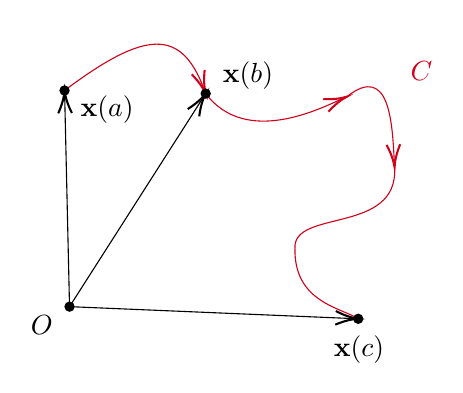
\begin{tikzpicture}[x=0.75pt,y=0.75pt,yscale=-1,xscale=1]
	%uncomment if require: \path (0,300); %set diagram left start at 0, and has height of 300
	
	%Curve Lines [id:da3276060381490892] 
	\draw [color={rgb, 255:red, 208; green, 2; blue, 27 }  ,draw opacity=1 ]   (176,103.75) .. controls (195.37,129.27) and (231.27,111.02) .. (242.33,105.98) ;
	\draw [shift={(244,105.25)}, rotate = 517.62] [color={rgb, 255:red, 208; green, 2; blue, 27 }  ,draw opacity=1 ][line width=0.75]    (10.93,-3.29) .. controls (6.95,-1.4) and (3.31,-0.3) .. (0,0) .. controls (3.31,0.3) and (6.95,1.4) .. (10.93,3.29)   ;
	%Curve Lines [id:da867110150451944] 
	\draw [color={rgb, 255:red, 208; green, 2; blue, 27 }  ,draw opacity=1 ]   (244,105.25) .. controls (264.86,88.76) and (265.95,118.37) .. (266.91,137.51) ;
	\draw [shift={(267,139.25)}, rotate = 266.99] [color={rgb, 255:red, 208; green, 2; blue, 27 }  ,draw opacity=1 ][line width=0.75]    (10.93,-3.29) .. controls (6.95,-1.4) and (3.31,-0.3) .. (0,0) .. controls (3.31,0.3) and (6.95,1.4) .. (10.93,3.29)   ;
	%Curve Lines [id:da48281776098084617] 
	\draw [color={rgb, 255:red, 208; green, 2; blue, 27 }  ,draw opacity=1 ]   (267,139.25) .. controls (269,171.75) and (218,159.25) .. (219,178.25) .. controls (218.5,204.25) and (241,206.75) .. (249.5,212.25) ;
	%Shape: Circle [id:dp01912153166389552] 
	\draw  [draw opacity=0][fill={rgb, 255:red, 0; green, 0; blue, 0 }  ,fill opacity=1 ] (107.9,206.4) .. controls (107.9,205.02) and (109.02,203.9) .. (110.4,203.9) .. controls (111.78,203.9) and (112.9,205.02) .. (112.9,206.4) .. controls (112.9,207.78) and (111.78,208.9) .. (110.4,208.9) .. controls (109.02,208.9) and (107.9,207.78) .. (107.9,206.4) -- cycle ;
	%Curve Lines [id:da9083644795099863] 
	\draw [color={rgb, 255:red, 208; green, 2; blue, 27 }  ,draw opacity=1 ]   (108,102.25) .. controls (147.2,72.85) and (164.31,72.26) .. (175.33,101.9) ;
	\draw [shift={(176,103.75)}, rotate = 250.75] [color={rgb, 255:red, 208; green, 2; blue, 27 }  ,draw opacity=1 ][line width=0.75]    (10.93,-3.29) .. controls (6.95,-1.4) and (3.31,-0.3) .. (0,0) .. controls (3.31,0.3) and (6.95,1.4) .. (10.93,3.29)   ;
	%Shape: Circle [id:dp4960073350824441] 
	\draw  [draw opacity=0][fill={rgb, 255:red, 0; green, 0; blue, 0 }  ,fill opacity=1 ] (105.5,102.25) .. controls (105.5,100.87) and (106.62,99.75) .. (108,99.75) .. controls (109.38,99.75) and (110.5,100.87) .. (110.5,102.25) .. controls (110.5,103.63) and (109.38,104.75) .. (108,104.75) .. controls (106.62,104.75) and (105.5,103.63) .. (105.5,102.25) -- cycle ;
	%Shape: Circle [id:dp8712280703593382] 
	\draw  [draw opacity=0][fill={rgb, 255:red, 0; green, 0; blue, 0 }  ,fill opacity=1 ] (173.5,103.75) .. controls (173.5,102.37) and (174.62,101.25) .. (176,101.25) .. controls (177.38,101.25) and (178.5,102.37) .. (178.5,103.75) .. controls (178.5,105.13) and (177.38,106.25) .. (176,106.25) .. controls (174.62,106.25) and (173.5,105.13) .. (173.5,103.75) -- cycle ;
	%Shape: Circle [id:dp9346879620682326] 
	\draw  [draw opacity=0][fill={rgb, 255:red, 0; green, 0; blue, 0 }  ,fill opacity=1 ] (247,212.25) .. controls (247,210.87) and (248.12,209.75) .. (249.5,209.75) .. controls (250.88,209.75) and (252,210.87) .. (252,212.25) .. controls (252,213.63) and (250.88,214.75) .. (249.5,214.75) .. controls (248.12,214.75) and (247,213.63) .. (247,212.25) -- cycle ;
	%Straight Lines [id:da3352312418861193] 
	\draw    (110.4,206.4) -- (247.5,212.17) ;
	\draw [shift={(249.5,212.25)}, rotate = 182.41] [color={rgb, 255:red, 0; green, 0; blue, 0 }  ][line width=0.75]    (10.93,-3.29) .. controls (6.95,-1.4) and (3.31,-0.3) .. (0,0) .. controls (3.31,0.3) and (6.95,1.4) .. (10.93,3.29)   ;
	%Straight Lines [id:da01233126994686784] 
	\draw    (110.4,206.4) -- (174.92,105.44) ;
	\draw [shift={(176,103.75)}, rotate = 482.58] [color={rgb, 255:red, 0; green, 0; blue, 0 }  ][line width=0.75]    (10.93,-3.29) .. controls (6.95,-1.4) and (3.31,-0.3) .. (0,0) .. controls (3.31,0.3) and (6.95,1.4) .. (10.93,3.29)   ;
	%Straight Lines [id:da11748387967404772] 
	\draw    (110.4,206.4) -- (108.05,104.25) ;
	\draw [shift={(108,102.25)}, rotate = 448.68] [color={rgb, 255:red, 0; green, 0; blue, 0 }  ][line width=0.75]    (10.93,-3.29) .. controls (6.95,-1.4) and (3.31,-0.3) .. (0,0) .. controls (3.31,0.3) and (6.95,1.4) .. (10.93,3.29)   ;
	
	% Text Node
	\draw (90.5,209.5) node [anchor=north west][inner sep=0.75pt]    {$O$};
	% Text Node
	\draw (114.5,103.5) node [anchor=north west][inner sep=0.75pt]    {$\mathbf{x}( a)$};
	% Text Node
	\draw (183,87.25) node [anchor=north west][inner sep=0.75pt]    {$\mathbf{x}( b)$};
	% Text Node
	\draw (236.5,219) node [anchor=north west][inner sep=0.75pt]    {$\mathbf{x}( c)$};
	% Text Node
	\draw (273.5,87) node [anchor=north west][inner sep=0.75pt]  [color={rgb, 255:red, 208; green, 2; blue, 27 }  ,opacity=1 ]  {$C$};
	
	
	\end{tikzpicture}

\end{center}

\begin{definition}[Differentiability and Smoothness]
	We say that a curve $C$ is \vocab{differentiable} if each of the components $\{x_1(t), x_2(t), x_3(t) \}$ are differentiable, and say $C$ is \vocab{regular} if $|\vv{x}'(t)| \neq 0$. If $C$ is differentiable and regular then we say $C$ is \vocab{smooth}.
\end{definition}

\begin{remark}
	The `regular' condition exists to avoid `spikes' in the curve. For example, consider the curve $\vv{x}(t) = (t^3, t^2)$. Clearly this is differentiable, but $\vv{x}(t)$ has a cusp at $t = 0$. At $t = 0$, we have $|\vv{x}'(0)| = 0$. If this was not the case, there would be no cusp.
\begin{center}
	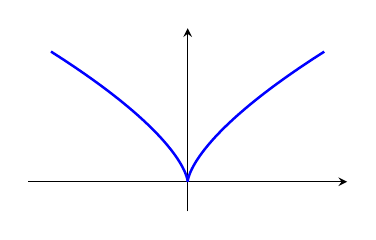
\begin{tikzpicture}[scale=1.5]
		\draw [->,>=stealth] (0, -0.25) -- (0, 1.3);
		\draw [->,>=stealth] (-1.35, 0) -- (1.35, 0);
		\draw [blue, line width=0.9pt, domain=-1.05:1.05, smooth, samples=81] plot ({\x*\x*\x}, {\x*\x});
	\end{tikzpicture}
\end{center}

\end{remark}


Recall that the function $x_i(t)$ is differentiable at $t$ if $x_i(t + h) = x_i(t) + x_i'(t) h + o(h)$, where $\frac{o(h)}{h} \rightarrow 0$ as $h \rightarrow 0$. We can write this in terms of vectors, where
$$
\vv{x}(t + h) = \vv{x}(t) + \vv{x}'(t)h + o(h),
$$
where $o(h)$ is a vector for which $\frac{|o(h)|}{h} \rightarrow 0$ as $h \rightarrow 0$.
  
Now given some curve $C$, we may want to find the length of the curve. We can try to do this by approximating the curve using straight lines.

\begin{center}
	

\tikzset{every picture/.style={line width=0.75pt}} %set default line width to 0.75pt        

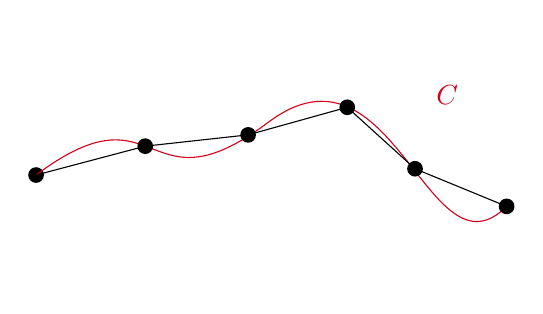
\begin{tikzpicture}[x=0.75pt,y=0.75pt,yscale=-1,xscale=1]
%uncomment if require: \path (0,300); %set diagram left start at 0, and has height of 300

%Shape: Ellipse [id:dp6464695455275871] 
\draw  [draw opacity=0][fill={rgb, 255:red, 0; green, 0; blue, 0 }  ,fill opacity=1 ] (42.5,126.68) .. controls (42.5,124.59) and (44.19,122.9) .. (46.28,122.9) .. controls (48.37,122.9) and (50.06,124.59) .. (50.06,126.68) .. controls (50.06,128.77) and (48.37,130.46) .. (46.28,130.46) .. controls (44.19,130.46) and (42.5,128.77) .. (42.5,126.68) -- cycle ;
%Curve Lines [id:da6916953701818653] 
\draw [color={rgb, 255:red, 208; green, 2; blue, 27 }  ,draw opacity=1 ]   (46.28,126.68) .. controls (106.73,81.34) and (97.66,146.63) .. (158.12,101.29) .. controls (218.57,55.95) and (235.2,179.58) .. (272.98,141.79) ;
%Shape: Circle [id:dp8157615548797015] 
\draw  [draw opacity=0][fill={rgb, 255:red, 0; green, 0; blue, 0 }  ,fill opacity=1 ] (95.09,112.77) .. controls (95.09,110.69) and (96.79,109) .. (98.87,109) .. controls (100.96,109) and (102.65,110.69) .. (102.65,112.77) .. controls (102.65,114.86) and (100.96,116.55) .. (98.87,116.55) .. controls (96.79,116.55) and (95.09,114.86) .. (95.09,112.77) -- cycle ;
%Shape: Ellipse [id:dp6623880161127722] 
\draw  [draw opacity=0][fill={rgb, 255:red, 0; green, 0; blue, 0 }  ,fill opacity=1 ] (144.67,107.33) .. controls (144.67,105.25) and (146.36,103.56) .. (148.45,103.56) .. controls (150.53,103.56) and (152.22,105.25) .. (152.22,107.33) .. controls (152.22,109.42) and (150.53,111.11) .. (148.45,111.11) .. controls (146.36,111.11) and (144.67,109.42) .. (144.67,107.33) -- cycle ;
%Shape: Ellipse [id:dp947023885876757] 
\draw  [draw opacity=0][fill={rgb, 255:red, 0; green, 0; blue, 0 }  ,fill opacity=1 ] (192.43,94.03) .. controls (192.43,91.95) and (194.12,90.26) .. (196.2,90.26) .. controls (198.29,90.26) and (199.98,91.95) .. (199.98,94.03) .. controls (199.98,96.12) and (198.29,97.81) .. (196.2,97.81) .. controls (194.12,97.81) and (192.43,96.12) .. (192.43,94.03) -- cycle ;
%Shape: Ellipse [id:dp9991347478656615] 
\draw  [draw opacity=0][fill={rgb, 255:red, 0; green, 0; blue, 0 }  ,fill opacity=1 ] (225.07,123.66) .. controls (225.07,121.57) and (226.76,119.88) .. (228.85,119.88) .. controls (230.94,119.88) and (232.63,121.57) .. (232.63,123.66) .. controls (232.63,125.74) and (230.94,127.43) .. (228.85,127.43) .. controls (226.76,127.43) and (225.07,125.74) .. (225.07,123.66) -- cycle ;
%Shape: Ellipse [id:dp5868702964474427] 
\draw  [draw opacity=0][fill={rgb, 255:red, 0; green, 0; blue, 0 }  ,fill opacity=1 ] (269.2,141.79) .. controls (269.2,139.71) and (270.89,138.01) .. (272.98,138.01) .. controls (275.07,138.01) and (276.76,139.71) .. (276.76,141.79) .. controls (276.76,143.88) and (275.07,145.57) .. (272.98,145.57) .. controls (270.89,145.57) and (269.2,143.88) .. (269.2,141.79) -- cycle ;
%Straight Lines [id:da7875885498839282] 
\draw    (46.28,126.68) -- (98.87,112.77) ;
%Straight Lines [id:da309124837435779] 
\draw    (98.87,112.77) -- (148.45,107.33) ;
%Straight Lines [id:da8902322155826599] 
\draw    (148.45,107.33) -- (196.2,94.03) ;
%Straight Lines [id:da9085782113625647] 
\draw    (196.2,94.03) -- (228.85,123.66) ;
%Straight Lines [id:da7165214688732946] 
\draw    (228.85,123.66) -- (272.98,141.79) ;

% Text Node
\draw (237.91,82.51) node [anchor=north west][inner sep=0.75pt]  [color={rgb, 255:red, 208; green, 2; blue, 27 }  ,opacity=1 ]  {$C$};


\end{tikzpicture}

\end{center}

For $C:[a, b] \rightarrow \R^3$ with $t \mapsto \vv{x}(t)$, we introduce a partition $P$ of $[a, b]$ with $t_0 = a$, $t_N = b$ and $t_0 < t_1 < \dots < t_N$, and we set $\Delta t_i = t_{i + 1} - t_i$ and $\Delta t = \max_i \Delta t_i$.

\begin{definition}[Length Relative to a Partition]
	For some curve $C$ and partition $P$ as above, we define the \vocab{length} of $C$ relative to $P$ by
	$$
	\ell(C, P) = \sum_{i = 0}^{N - 1} \left|\vv{x}(t_{i + 1}) - \vv{x}(t_i)\right|.
$$
\end{definition}

We would expect that this length would get closer to the true length of $C$ as $\Delta t \rightarrow 0$. Indeed, we will define the length of $C$ in this way.

\begin{definition}[Length of a Curve]
	We define the length of a curve $C$ by
	$$
	\ell(C) = \lim_{\Delta t \to 0} \sum_{i = 0}^{N - 1} \left|\vv{x}(t_{i + 1}) - \vv{x}(t_i) \right| = \lim_{\Delta t \rightarrow 0} \ell(C, P).
	$$
	If this limit does not exist, we say the curve is \vocab{non-rectifiable}.
\end{definition}

In this course, we will not worry too much about non-rectifiable curves, so we will assume that this notion is always well defined.

Now suppose $C$ is a differentiable curve. Then we have that
\begin{align*}
	\vv{x}(t_{i + 1}) &= \vv{x}(t_i + t_{i + 1} - t_i) \\
					&= \vv{x}(t_i + \Delta t_i) \\
					&= \vv{x}(t_i) + \vv{x}'(t_i) \Delta t_i + o(\Delta t_i).
\end{align*}
It follows that
$$
|\vv{x}(t_{i + 1}) - \vv{x}(t_i) | = |\vv{x}'(t_i)| \Delta t_i + o(\Delta t_i). 
$$

So if $C$ is differentiable, we get the expression
$$
\ell(C, P)=\sum_{i=0}^{N-1}\left(\left|\mathbf{x}^{\prime}\left(t_{i}\right)\right| \Delta t_{i}+o\left(\Delta t_{i}\right)\right).
$$
Recall that $o(\Delta t_i)$ represents a function for which $\frac{o(\Delta t_i)}{\Delta t_i} \rightarrow 0$ as $\Delta t_i \rightarrow 0$. So for any $\epsilon > 0$, if $\Delta t = \max_i \Delta t_i$  is sufficiently small, then we have
$$
|o(\Delta t_i) | < \left(\frac{\epsilon}{b - a}\right) \Delta t_i,
$$
for $i = \{0, \dots, N - 1\}$. So
\begin{align*}
	\left|\ell(C, P) - \sum_{i = 0}^{N - 1} |\vv{x}' (t_i)| \Delta t_i \right| &= \left|\sum_{i = 0}^{N - 1} o(\Delta t_i)\right| \\
	&< \frac{\epsilon}{b - a} \sum_{i = 0}^{N - 1} \Delta{t_i} = \epsilon.
\end{align*}
Thus the LHS tends to zero as $\Delta t \rightarrow 0$. So we get that
\begin{align*}
	\ell(C) &= \lim_{\Delta t \to 0} \ell(C, P) = \lim_{\Delta t \to 0} \sum_{i = 0}^{N - 1} |\vv{x}'(t_i)| \Delta t_i \\
		&= \int_a^b \left|\vv{x}'(t)\right| \; \dd t,
\end{align*}
by the definition of the Riemann integral.
So, we can restate our definition in this other form.

\begin{definition}[Length of a Curve]
	If $C: [a, b] \rightarrow \R^3$ is a differentiable curve with $t \mapsto \vv{x}(t)$, then its \vocab{length} is
	$$
	\ell(C) = \int_a^b |\vv{x}'(t)| \; \dd t = \int_C \dd s,
	$$
where $\dd s$ is the \vocab{arc-length element}, $\dd s = |\vv{x}'(t)| \; \dd t$.
\end{definition}

With this defined, we can define the integral of a function along a curve.

\begin{definition}[Integral on a Curve]
	For a function $f : \R^3 \rightarrow \R$ and a differentiable curve $C: [a, b] \rightarrow \R^3$ with $t \mapsto \vv{x}(t)$, we define the \vocab{integral of $f$ along $C$} to be
	$$
	\int_C f(\vv{x})\; \dd s = \int_a^b f(\vv{x}(t)) |\vv{x}'(t)| \; \dd t.
	$$
\end{definition}

Now consider a curve $C$ made up of $M$ smooth curves $C_1, C_2, \dots, C_M$.

\begin{center}
	

\tikzset{every picture/.style={line width=0.75pt}} %set default line width to 0.75pt        

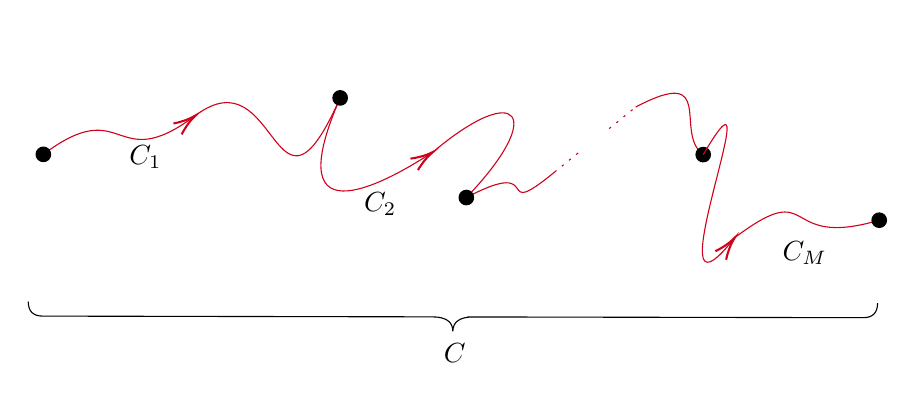
\begin{tikzpicture}[x=0.75pt,y=0.75pt,yscale=-1,xscale=1]
%uncomment if require: \path (0,300); %set diagram left start at 0, and has height of 300

%Curve Lines [id:da5796763237473451] 
\draw [color={rgb, 255:red, 208; green, 2; blue, 27 }  ,draw opacity=1 ]   (37.48,39.48) .. controls (77.08,9.78) and (71.01,49.86) .. (109.69,21.56) ;
\draw [shift={(110.88,20.68)}, rotate = 503.13] [color={rgb, 255:red, 208; green, 2; blue, 27 }  ,draw opacity=1 ][line width=0.75]    (10.93,-3.29) .. controls (6.95,-1.4) and (3.31,-0.3) .. (0,0) .. controls (3.31,0.3) and (6.95,1.4) .. (10.93,3.29)   ;
%Curve Lines [id:da30640590954836433] 
\draw [color={rgb, 255:red, 208; green, 2; blue, 27 }  ,draw opacity=1 ]   (110.88,20.68) .. controls (150.88,-9.32) and (148.48,84.28) .. (180.48,12.28) ;
%Curve Lines [id:da18452242492784054] 
\draw [color={rgb, 255:red, 208; green, 2; blue, 27 }  ,draw opacity=1 ]   (180.48,12.28) .. controls (148.83,84.85) and (206.94,50.14) .. (223.63,39.35) ;
\draw [shift={(225.28,38.28)}, rotate = 506.69] [color={rgb, 255:red, 208; green, 2; blue, 27 }  ,draw opacity=1 ][line width=0.75]    (10.93,-3.29) .. controls (6.95,-1.4) and (3.31,-0.3) .. (0,0) .. controls (3.31,0.3) and (6.95,1.4) .. (10.93,3.29)   ;
%Curve Lines [id:da1500064698451402] 
\draw [color={rgb, 255:red, 208; green, 2; blue, 27 }  ,draw opacity=1 ]   (225.28,38.28) .. controls (266.08,3.88) and (280.08,19.88) .. (241.28,60.28) ;
%Shape: Ellipse [id:dp3321298680409044] 
\draw  [draw opacity=0][fill={rgb, 255:red, 0; green, 0; blue, 0 }  ,fill opacity=1 ] (176.7,12.28) .. controls (176.7,10.19) and (178.39,8.5) .. (180.48,8.5) .. controls (182.57,8.5) and (184.26,10.19) .. (184.26,12.28) .. controls (184.26,14.37) and (182.57,16.06) .. (180.48,16.06) .. controls (178.39,16.06) and (176.7,14.37) .. (176.7,12.28) -- cycle ;
%Shape: Ellipse [id:dp5859967156381527] 
\draw  [draw opacity=0][fill={rgb, 255:red, 0; green, 0; blue, 0 }  ,fill opacity=1 ] (33.7,39.48) .. controls (33.7,37.39) and (35.39,35.7) .. (37.48,35.7) .. controls (39.57,35.7) and (41.26,37.39) .. (41.26,39.48) .. controls (41.26,41.57) and (39.57,43.26) .. (37.48,43.26) .. controls (35.39,43.26) and (33.7,41.57) .. (33.7,39.48) -- cycle ;
%Curve Lines [id:da9173421636172133] 
\draw [color={rgb, 255:red, 208; green, 2; blue, 27 }  ,draw opacity=1 ]   (241.28,60.28) .. controls (280.6,39.6) and (253,73.2) .. (283.8,48) ;
%Shape: Ellipse [id:dp4659247920376307] 
\draw  [draw opacity=0][fill={rgb, 255:red, 0; green, 0; blue, 0 }  ,fill opacity=1 ] (237.5,60.28) .. controls (237.5,58.19) and (239.19,56.5) .. (241.28,56.5) .. controls (243.37,56.5) and (245.06,58.19) .. (245.06,60.28) .. controls (245.06,62.37) and (243.37,64.06) .. (241.28,64.06) .. controls (239.19,64.06) and (237.5,62.37) .. (237.5,60.28) -- cycle ;
%Straight Lines [id:da8487824909604982] 
\draw [color={rgb, 255:red, 208; green, 2; blue, 27 }  ,draw opacity=1 ] [dash pattern={on 0.84pt off 2.51pt}]  (283.8,48) -- (296.6,37.6) ;
%Curve Lines [id:da5732848696347904] 
\draw [color={rgb, 255:red, 208; green, 2; blue, 27 }  ,draw opacity=1 ]   (322.88,16.68) .. controls (362.2,-4) and (341,29.2) .. (355.4,39.6) ;
%Straight Lines [id:da9728872621803147] 
\draw [color={rgb, 255:red, 208; green, 2; blue, 27 }  ,draw opacity=1 ] [dash pattern={on 0.84pt off 2.51pt}]  (310.08,27.08) -- (322.88,16.68) ;
%Shape: Ellipse [id:dp6071568671300255] 
\draw  [draw opacity=0][fill={rgb, 255:red, 0; green, 0; blue, 0 }  ,fill opacity=1 ] (351.62,39.6) .. controls (351.62,37.51) and (353.31,35.82) .. (355.4,35.82) .. controls (357.49,35.82) and (359.18,37.51) .. (359.18,39.6) .. controls (359.18,41.69) and (357.49,43.38) .. (355.4,43.38) .. controls (353.31,43.38) and (351.62,41.69) .. (351.62,39.6) -- cycle ;
%Curve Lines [id:da29258101011575044] 
\draw [color={rgb, 255:red, 208; green, 2; blue, 27 }  ,draw opacity=1 ]   (355.4,39.6) .. controls (391.22,-21.29) and (328.04,132.85) .. (369.96,80.41) ;
\draw [shift={(370.6,79.6)}, rotate = 488.25] [color={rgb, 255:red, 208; green, 2; blue, 27 }  ,draw opacity=1 ][line width=0.75]    (10.93,-3.29) .. controls (6.95,-1.4) and (3.31,-0.3) .. (0,0) .. controls (3.31,0.3) and (6.95,1.4) .. (10.93,3.29)   ;
%Curve Lines [id:da6819173648579594] 
\draw [color={rgb, 255:red, 208; green, 2; blue, 27 }  ,draw opacity=1 ]   (370.6,79.6) .. controls (410.6,49.6) and (391.4,85.6) .. (440.2,71.2) ;
%Shape: Ellipse [id:dp5818550932291585] 
\draw  [draw opacity=0][fill={rgb, 255:red, 0; green, 0; blue, 0 }  ,fill opacity=1 ] (436.42,71.2) .. controls (436.42,69.11) and (438.11,67.42) .. (440.2,67.42) .. controls (442.29,67.42) and (443.98,69.11) .. (443.98,71.2) .. controls (443.98,73.29) and (442.29,74.98) .. (440.2,74.98) .. controls (438.11,74.98) and (436.42,73.29) .. (436.42,71.2) -- cycle ;
%Shape: Brace [id:dp414059666657298] 
\draw   (30.2,110.4) .. controls (30.19,115.07) and (32.52,117.4) .. (37.19,117.41) -- (224.79,117.77) .. controls (231.46,117.78) and (234.78,120.12) .. (234.77,124.79) .. controls (234.78,120.12) and (238.12,117.8) .. (244.79,117.81)(241.79,117.81) -- (432.39,118.17) .. controls (437.06,118.18) and (439.39,115.86) .. (439.4,111.19) ;

% Text Node
\draw (77.6,34) node [anchor=north west][inner sep=0.75pt]    {$C_{1}$};
% Text Node
\draw (190.8,56.4) node [anchor=north west][inner sep=0.75pt]    {$C_{2}$};
% Text Node
\draw (229.2,129.6) node [anchor=north west][inner sep=0.75pt]    {$C$};
% Text Node
\draw (392.4,80.4) node [anchor=north west][inner sep=0.75pt]    {$C_{M}$};


\end{tikzpicture}

\end{center}

Then writing $C = C_1 + C_2 + \cdots + C_M$, we can define
$$
\int_C f(\vv{x}) \; \dd s = \sum_{i = 1}^M \int_{C_i} f(\vv{x}) \; \dd s,
$$
so we can integrate over piecewise smooth curves.

Note that informally, we have 
$$\dd s = |\vv{x}'(t)| \; \dd t = \sqrt{\left(\frac{\dd x}{\dd t}\right)^2 + \left(\frac{\dd y}{\dd t}\right)^2 + \left(\frac{\dd z}{\dd t}\right)^2} \; \dd t.$$
So being somewhat sacrilegious, we have
$$
\dd s^2 = \dd x^2 + \dd y^2 + \dd z^2.
$$

\begin{example}[Circumference of a Circle]
	Let $C$ be a circle of radius $r > 0$ in $\R^3$,
	$$
	\vv{x}(t) = \begin{pmatrix}
		r \cos t \\
		r \sin t \\
		0
	\end{pmatrix}, \quad \quad t \in [0, 2 \pi].
	$$
	We can differentiate this to get 
	$$
	\vv{x}'(t) = \begin{pmatrix}
		-r \sin t \\
		r \cos t \\
		0
	\end{pmatrix}, \quad \quad t \in [0, 2 \pi].
	$$
	Then integrating over $C$ we have
	\begin{align*}
		\int_C \; \dd s &= \int_0^{2 \pi} \sqrt{r^2 \sin^2 t + r^2 \cos^2 t} \; \dd t\\
		&= \int_0^{2 \pi} r \; \dd t \\
		&= 2 \pi r,
	\end{align*}
	as we would expect.
\end{example}

\begin{example}[Integrating over a Circle]
	With $C$ being a circle as before, we can integrate over the curve. For example
	\begin{align*}
		\int_C x^2 y \; \dd s &= \int_0^{2 \pi} (r \cos t)^2 (r \sin t) \underbrace{r \; \dd t}_{|\vv{x}'(t)| \; \dd t} \\
		&= 0
	\end{align*}
\end{example}

There is one subtlety that we have looked over - does $\ell(C)$ depend on the parameterization used?

For example, if we had $\vv{x}(t) = (r \cos t, r \sin t, 0)$ with $t \in [0, 2 \pi]$ and $\tilde{\vv{x}}(t) = (r \cos(2 t), r \sin(2 t), 0)$ with $t \in [0, \pi]$, these represent the same circle and they should have the same length. We will clear up this possible ambiguity now.

\begin{proposition}
	If $f:\R^3 \rightarrow \R$ is a function and $C$ is a differentiable curve, then $\int_C f(\vv{x}) \; \dd s$ is independent of the parameterization of $C$ used.
\end{proposition}
\begin{proof}
Suppose $C$ has two different parameterizations,
\begin{align*}
	\vv{x} &= \vv{x}_1(t), \quad \quad a \leq t \leq b \\
	\vv{x} &= \vv{x}_2(t), \quad \quad \alpha \leq t \leq \beta
\end{align*}
We must then have $\vv{x}_2(\tau) = \vv{x}_1(t(\tau))$ for some function $t(\tau)$. We can assume that $\frac{\dd t}{\dd \tau} \neq 0$ so the map between $t$ and $\tau$ is invertible and differentiable (this is the inverse function theorem, covered in Analysis and Topology in Part IB). Note then that 
\begin{align*}
	\vv{x}'_2(\tau) &= \frac{\dd}{\dd\tau} \vv{x}_2(t) \\
	&= \frac{\dd} {\dd \tau} \vv{x}_1(t(\tau)) \\
	&= \frac{\dd t}{\dd \tau} \vv{x}_1'(t(\tau)).
\end{align*}
Then from our definition,
$$
\int_C f(\vv{x}) \; \dd s = \int_{a}^b f(\vv{x}_1(t)) |\vv{x}_1'(t)| \; \dd t.
$$
We can make the substitution $t = t(\tau)$, and assuming $\dd t/\dd\tau > 0$, the latter integral becomes
$$
\int_\alpha^\beta f(\vv{x}_2(\tau)) \underbrace{|\vv{x}_1'(t(\tau))| \frac{\dd t}{\dd \tau} \;\dd \tau}_{|\vv{x}'_2 (\tau)| \; \dd\tau},
$$
which is precisely the same as $\int_C f(\vv{x}) \; \dd s$ using the $\vv{x}_2(t)$ parameterization. 

We assumed here that $\frac{\dd t}{\dd \tau} > 0$, but the same holds if it is negative. Thus our definition of integrating over a curve $C$ does not depend on the choice of parameterization of $C$.
\end{proof}

We can parameterize curves in many different ways. One useful way to parameterise regular curves is with respect to arc-length.
If we write $\vv{r}(s) = \vv{x}(t(s))$ where $0 \leq s \leq \ell(C)$, then by the chain rule
$$
	\frac{\dd t}{\dd s} = \frac{1}{\dd s/ \dd t} = \frac{1}{|\vv{x}'(t(s))|},
$$
so
\begin{align*}
	\vv{r}'(s) &= \frac{\dd}{\dd s} \vv{x}(t(s)) \\
	&= \frac{\dd t}{\dd s} \vv{x}'(t(s)) \\
	&= \frac{\vv{x}'(t(s))}{|\vv{x}'(t(s))|},
\end{align*}
that is, $|\vv{r}'(s)| = 1$. This (consistently) gives $\ell(C) = \int_0^{\ell(C)} |\vv{r}'(s)| \; \dd s = \int_0^{\ell(C)} \; \dd s$.
So the way to picture $\vv{r}'(s)$ is as the unit tangent vector to the curve.

\begin{center}
	

\tikzset{every picture/.style={line width=0.75pt}} %set default line width to 0.75pt        

\begin{tikzpicture}[x=0.75pt,y=0.75pt,yscale=-1,xscale=1]
%uncomment if require: \path (0,300); %set diagram left start at 0, and has height of 300

%Shape: Ellipse [id:dp6228782401096558] 
\draw  [draw opacity=0][fill={rgb, 255:red, 0; green, 0; blue, 0 }  ,fill opacity=1 ] (158.04,210.31) .. controls (158.04,208.37) and (159.61,206.8) .. (161.54,206.8) .. controls (163.48,206.8) and (165.05,208.37) .. (165.05,210.31) .. controls (165.05,212.24) and (163.48,213.81) .. (161.54,213.81) .. controls (159.61,213.81) and (158.04,212.24) .. (158.04,210.31) -- cycle ;
%Straight Lines [id:da8695480911058163] 
\draw    (161.54,210.31) -- (156.84,56.82) ;
\draw [shift={(156.78,54.82)}, rotate = 448.24] [color={rgb, 255:red, 0; green, 0; blue, 0 }  ][line width=0.75]    (10.93,-3.29) .. controls (6.95,-1.4) and (3.31,-0.3) .. (0,0) .. controls (3.31,0.3) and (6.95,1.4) .. (10.93,3.29)   ;
%Curve Lines [id:da8139461687050455] 
\draw [color={rgb, 255:red, 208; green, 2; blue, 27 }  ,draw opacity=1 ]   (67.05,164.18) .. controls (64.24,127.73) and (111.91,53.42) .. (158.18,54.82) .. controls (204.45,56.22) and (203.05,168.39) .. (291.38,95.48) ;
%Straight Lines [id:da9732872849600818] 
\draw    (161.54,210.31) -- (68.84,165.06) ;
\draw [shift={(67.05,164.18)}, rotate = 386.02] [color={rgb, 255:red, 0; green, 0; blue, 0 }  ][line width=0.75]    (10.93,-3.29) .. controls (6.95,-1.4) and (3.31,-0.3) .. (0,0) .. controls (3.31,0.3) and (6.95,1.4) .. (10.93,3.29)   ;
%Straight Lines [id:da38328258500214996] 
\draw [color={rgb, 255:red, 74; green, 144; blue, 226 }  ,draw opacity=1 ]   (67.05,164.18) -- (63.55,117.52) ;
\draw [shift={(63.4,115.53)}, rotate = 445.71] [color={rgb, 255:red, 74; green, 144; blue, 226 }  ,draw opacity=1 ][line width=0.75]    (10.93,-3.29) .. controls (6.95,-1.4) and (3.31,-0.3) .. (0,0) .. controls (3.31,0.3) and (6.95,1.4) .. (10.93,3.29)   ;
%Straight Lines [id:da8330115590680308] 
\draw [color={rgb, 255:red, 74; green, 144; blue, 226 }  ,draw opacity=1 ]   (156.78,54.82) -- (204.97,57.65) ;
\draw [shift={(206.97,57.76)}, rotate = 183.36] [color={rgb, 255:red, 74; green, 144; blue, 226 }  ,draw opacity=1 ][line width=0.75]    (10.93,-3.29) .. controls (6.95,-1.4) and (3.31,-0.3) .. (0,0) .. controls (3.31,0.3) and (6.95,1.4) .. (10.93,3.29)   ;

% Text Node
\draw (163.54,213.31) node [anchor=north west][inner sep=0.75pt]    {$O$};
% Text Node
\draw (293.38,98.48) node [anchor=north west][inner sep=0.75pt]  [color={rgb, 255:red, 208; green, 2; blue, 27 }  ,opacity=1 ]  {$C$};
% Text Node
\draw (94.62,190.95) node [anchor=north west][inner sep=0.75pt]  [color={rgb, 255:red, 0; green, 0; blue, 0 }  ,opacity=1 ]  {$\mathbf{r}( 0)$};
% Text Node
\draw (32.22,92.95) node [anchor=north west][inner sep=0.75pt]  [color={rgb, 255:red, 74; green, 144; blue, 226 }  ,opacity=1 ]  {$\mathbf{r} '( 0)$};
% Text Node
\draw (160.62,30.55) node [anchor=north west][inner sep=0.75pt]  [color={rgb, 255:red, 74; green, 144; blue, 226 }  ,opacity=1 ]  {$\mathbf{r} '( s)$};
% Text Node
\draw (161.82,115.75) node [anchor=north west][inner sep=0.75pt]  [color={rgb, 255:red, 74; green, 144; blue, 226 }  ,opacity=1 ]  {$\mathbf{r}( s)$};


\end{tikzpicture}

\end{center}

\subsection{Curvature and Torsion}

Throughout this section, 
we  will talk about a generic regular curve $C$, parameterized by arc-length, and we will write $s \mapsto \vv{r}(s).$

\begin{definition}[Tangent Vector]
	For a regular curve $C$ parameterized by arc length, we define the \vocab{tangent vector} to be $\vv{t}(s) = \vv{r}'(s)$.
\end{definition}

We already established that $|\vv{t}(s)| = 1$, and thus as the second derivative $\vv{r}''(s) = \vv{t}'(s)$ only measures the change in \emph{direction}.

Intuitively, if $|\vv{r}''(s)|$ is large, then the curve rapidly changes in direction, whereas if $|\vv{r}''(s)|$ is small, we would expect the curve to be approximately flat.

\begin{definition}[Curvature]
	We define the \vocab{curvature} of $C$ to be $\kappa(s) = |\vv{r}''(s)| = |\vv{t}'(s)|$.
\end{definition}
\begin{center}
	

\tikzset{every picture/.style={line width=0.75pt}} %set default line width to 0.75pt        

\begin{tikzpicture}[x=0.75pt,y=0.75pt,yscale=-1,xscale=1]
%uncomment if require: \path (0,300); %set diagram left start at 0, and has height of 300

%Curve Lines [id:da6272470901360102] 
\draw [color={rgb, 255:red, 208; green, 2; blue, 27 }  ,draw opacity=1 ]   (47,107.6) .. controls (69,113.1) and (130.6,82.2) .. (140,86.5) .. controls (149.4,90.8) and (9.2,128.2) .. (40.2,131.2) ;
%Shape: Circle [id:dp23011696399122117] 
\draw  [color={rgb, 255:red, 0; green, 0; blue, 0 }  ,draw opacity=1 ][dash pattern={on 4.5pt off 4.5pt}] (127.5,86.5) .. controls (127.5,79.6) and (133.1,74) .. (140,74) .. controls (146.9,74) and (152.5,79.6) .. (152.5,86.5) .. controls (152.5,93.4) and (146.9,99) .. (140,99) .. controls (133.1,99) and (127.5,93.4) .. (127.5,86.5) -- cycle ;
%Curve Lines [id:da8187188453621865] 
\draw [color={rgb, 255:red, 208; green, 2; blue, 27 }  ,draw opacity=1 ]   (299.8,102) .. controls (339.4,88) and (415.8,132.4) .. (455.8,102.4) ;
%Shape: Circle [id:dp5617098266931536] 
\draw  [color={rgb, 255:red, 0; green, 0; blue, 0 }  ,draw opacity=1 ][dash pattern={on 4.5pt off 4.5pt}] (363.1,105.7) .. controls (363.1,98.8) and (368.7,93.2) .. (375.6,93.2) .. controls (382.5,93.2) and (388.1,98.8) .. (388.1,105.7) .. controls (388.1,112.6) and (382.5,118.2) .. (375.6,118.2) .. controls (368.7,118.2) and (363.1,112.6) .. (363.1,105.7) -- cycle ;

% Text Node
\draw (148.6,52.4) node [anchor=north west][inner sep=0.75pt]   [align=left] {$\displaystyle \kappa ( s)$ large};
% Text Node
\draw (379,65.2) node [anchor=north west][inner sep=0.75pt]   [align=left] {$\displaystyle \kappa ( s)$ small};


\end{tikzpicture}

\end{center}

Now since $\vv{t} = \vv{r}'(s)$ is a unit vector, if we differentiate $\vv{t} \cdot \vv{t} = 1$ we get $\vv{t} \cdot \vv{t}' = 0$. Because of this we can introduce the following definition.

\begin{definition}[Principal Normal]
	The \vocab{principal normal} $\vv{n}$ is the vector given by $\vv{t}' = \kappa \vv{n}$.
\end{definition}

The principal normal $\vv{n}$ is everywhere normal to the curve $C$, since it's always perpendicular to the tangent vector ($\vv{t} \cdot \vv{n} = 0$). Then we have two perpendicular vectors, so we can extend $\{\vv{t}, \vv{n}\}$ to an orthonormal basis by defining the following.

\begin{definition}[Binormal]
	The \vocab{binormal} $\vv{b}$ is the unit vector perpendicular to $\vv{t}$ and $\vv{n}$, $\vv{b} = \vv{t} \times \vv{n}$. 
\end{definition}

Since $|\vv{b}| = 1$, we have $\vv{b}' \cdot \vv{b} = 0$. Also since $\vv{t} \cdot \vv{b} = 0$ and $\vv{n} \cdot \vv{b} = 0$,
\begin{align*}
	0 &= (\vv{t} \cdot \vv{b})' = \vv{t}' \cdot \vv{b} + \vv{t} \cdot \vv{b}'  \\
	&= \cancel{\kappa \vv{n} \cdot \vv{b}} + \vv{t} \cdot \vv{b}',
\end{align*}
thus $\vv{b}'$ is orthogonal to $\vv{t}$ and $\vv{b}$, and thus it is parallel to $\vv{n}$. We define the following.

\begin{definition}[Torsion]
	We define the \vocab{torsion} $\tau$ by $\vv{b}' = - \tau \vv{n}$.
\end{definition}

Informally, torsion measures a twisting motion along a curve.
So we have two equations.
$$
\vv{t}' = \kappa \vv{n}, \quad \quad \vv{b}' = - \tau \vv{n}.
$$

\begin{proposition}[Fundamental Theorem of Curves]
	The curvature $\kappa(s)$ and torsion $\tau(s)$ define a curve up to translation and orientation.
\end{proposition}
\begin{proof}[Proof Sketch]
	Since $\vv{n} = \vv{b} \times \vv{t}$, we have
	$$
	\vv{t}' = \kappa (\vv{b} \times \vv{t}), \quad \vv{b}' = - \tau (\vv{b} \times \vv{t}).
	$$
	This gives six equations for six unknowns. Given $\kappa(s)$, $\tau(s)$, $\vv{t}(0)$ and $\vv{b}(0)$, we can construct the functions $\vv{t}(s)$, $\vv{b}(s)$, and hence $\vv{n} = \vv{b} \times \vv{t}$. Hence the result.
\end{proof}

\subsection{Radius of Curvature}

Consider some generic curve $s \mapsto \vv{r}(s)$, and consider the Taylor expansion about $s = 0$. Write $\vv{t} = \vv{t}(0)$, $\vv{n} = \vv{n}(0)$, etc. Then we get
\begin{align*}
	\vv{r}(s) &= \vv{r}(0) + s\vv{r}'(0) + \frac{1}{2}s^2 \vv{r}''(0) + o(s^2) \\
	&= \vv{r} + s\vv{t} + \frac{1}{2}s^2 \kappa \vv{n}	+ o(s^2).
\end{align*}
So this gives us a good approximation of the curve around $s = 0$, and now we want to try and draw a circle through the point $\vv{r}(0)$ such that the circle is tangent to the curve at that point. Specifically, what would the radius of that circle be?

Suppose, without loss of generality, that $\vv{t}$ is horizontal.

\begin{center}
	


	\tikzset{every picture/.style={line width=0.75pt}} %set default line width to 0.75pt        

	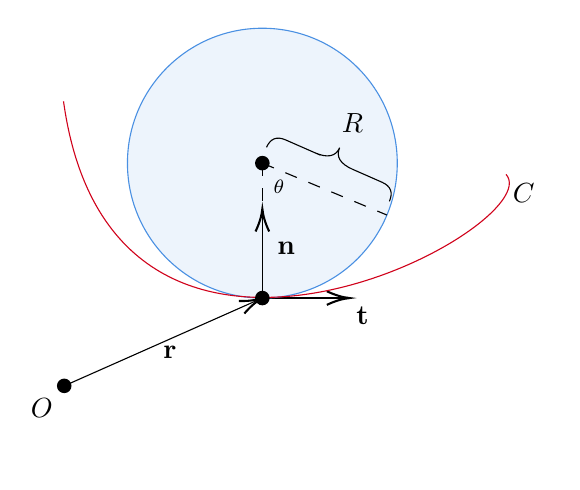
\begin{tikzpicture}[x=0.75pt,y=0.75pt,yscale=-1,xscale=1]
	%uncomment if require: \path (0,300); %set diagram left start at 0, and has height of 300
	
	%Shape: Ellipse [id:dp11623285715454001] 
	\draw  [draw opacity=0][fill={rgb, 255:red, 0; green, 0; blue, 0 }  ,fill opacity=1 ] (161.04,202.31) .. controls (161.04,200.37) and (162.61,198.8) .. (164.54,198.8) .. controls (166.48,198.8) and (168.05,200.37) .. (168.05,202.31) .. controls (168.05,204.24) and (166.48,205.81) .. (164.54,205.81) .. controls (162.61,205.81) and (161.04,204.24) .. (161.04,202.31) -- cycle ;
	%Straight Lines [id:da2508934300022321] 
	\draw    (164.54,202.31) -- (258.17,160.81) ;
	\draw [shift={(260,160)}, rotate = 516.1] [color={rgb, 255:red, 0; green, 0; blue, 0 }  ][line width=0.75]    (10.93,-3.29) .. controls (6.95,-1.4) and (3.31,-0.3) .. (0,0) .. controls (3.31,0.3) and (6.95,1.4) .. (10.93,3.29)   ;
	%Straight Lines [id:da7674997790762081] 
	\draw [color={rgb, 255:red, 0; green, 0; blue, 0 }  ,draw opacity=1 ]   (260,160) -- (300,160) ;
	\draw [shift={(302,160)}, rotate = 180] [color={rgb, 255:red, 0; green, 0; blue, 0 }  ,draw opacity=1 ][line width=0.75]    (10.93,-3.29) .. controls (6.95,-1.4) and (3.31,-0.3) .. (0,0) .. controls (3.31,0.3) and (6.95,1.4) .. (10.93,3.29)   ;
	%Shape: Circle [id:dp6348939130079169] 
	\draw  [color={rgb, 255:red, 74; green, 144; blue, 226 }  ,draw opacity=1 ][fill={rgb, 255:red, 74; green, 144; blue, 226 }  ,fill opacity=0.1 ] (195,95) .. controls (195,59.1) and (224.1,30) .. (260,30) .. controls (295.9,30) and (325,59.1) .. (325,95) .. controls (325,130.9) and (295.9,160) .. (260,160) .. controls (224.1,160) and (195,130.9) .. (195,95) -- cycle ;
	%Straight Lines [id:da4205464127260875] 
	\draw [draw opacity=0]   (260,95) -- (260,160) ;
	\draw [shift={(260,160)}, rotate = 90] [draw opacity=0][line width=0.75]      (0, 0) circle [x radius= 3.35, y radius= 3.35]   ;
	\draw [shift={(260,95)}, rotate = 90] [draw opacity=0][line width=0.75]      (0, 0) circle [x radius= 3.35, y radius= 3.35]   ;
	%Straight Lines [id:da5779811168879634] 
	\draw  [dash pattern={on 4.5pt off 4.5pt}]  (260,95) -- (320,120) ;
	%Straight Lines [id:da25785735111397157] 
	\draw [color={rgb, 255:red, 0; green, 0; blue, 0 }  ,draw opacity=1 ]   (260,160) -- (260,119) ;
	\draw [shift={(260,117)}, rotate = 450] [color={rgb, 255:red, 0; green, 0; blue, 0 }  ,draw opacity=1 ][line width=0.75]    (10.93,-3.29) .. controls (6.95,-1.4) and (3.31,-0.3) .. (0,0) .. controls (3.31,0.3) and (6.95,1.4) .. (10.93,3.29)   ;
	%Shape: Ellipse [id:dp504146351430413] 
	\draw  [draw opacity=0][fill={rgb, 255:red, 0; green, 0; blue, 0 }  ,fill opacity=1 ] (256.49,95) .. controls (256.49,93.06) and (258.06,91.49) .. (260,91.49) .. controls (261.94,91.49) and (263.51,93.06) .. (263.51,95) .. controls (263.51,96.94) and (261.94,98.51) .. (260,98.51) .. controls (258.06,98.51) and (256.49,96.94) .. (256.49,95) -- cycle ;
	%Curve Lines [id:da3234174981600959] 
	\draw [color={rgb, 255:red, 208; green, 2; blue, 27 }  ,draw opacity=1 ]   (164.2,65.2) .. controls (188.2,238.8) and (399.4,124.8) .. (377.4,100.4) ;
	%Shape: Ellipse [id:dp9921539771179669] 
	\draw  [draw opacity=0][fill={rgb, 255:red, 0; green, 0; blue, 0 }  ,fill opacity=1 ] (256.49,160) .. controls (256.49,158.06) and (258.06,156.49) .. (260,156.49) .. controls (261.94,156.49) and (263.51,158.06) .. (263.51,160) .. controls (263.51,161.94) and (261.94,163.51) .. (260,163.51) .. controls (258.06,163.51) and (256.49,161.94) .. (256.49,160) -- cycle ;
	%Shape: Brace [id:dp6625426388074377] 
	\draw   (321.2,113.4) .. controls (323.07,109.13) and (321.88,106.05) .. (317.61,104.18) -- (303.57,98.01) .. controls (297.46,95.33) and (295.35,91.85) .. (297.23,87.58) .. controls (295.35,91.85) and (291.36,92.65) .. (285.26,89.97)(288.01,91.18) -- (271.22,83.81) .. controls (266.95,81.93) and (263.87,83.13) .. (262,87.4) ;
	%Straight Lines [id:da3029069687640311] 
	\draw  [dash pattern={on 4.5pt off 4.5pt}]  (260,95) -- (260,117) ;
	
	% Text Node
	\draw (379.4,103.4) node [anchor=north west][inner sep=0.75pt]    {$C$};
	% Text Node
	\draw (147.2,207.2) node [anchor=north west][inner sep=0.75pt]    {$O$};
	% Text Node
	\draw (211,182) node [anchor=north west][inner sep=0.75pt]    {$\mathbf{r}$};
	% Text Node
	\draw (304,163) node [anchor=north west][inner sep=0.75pt]  [color={rgb, 255:red, 0; green, 0; blue, 0 }  ,opacity=1 ]  {$\mathbf{t}$};
	% Text Node
	\draw (264,102) node [anchor=north west][inner sep=0.75pt]  [font=\scriptsize]  {$\theta $};
	% Text Node
	\draw (266,132) node [anchor=north west][inner sep=0.75pt]  [color={rgb, 255:red, 0; green, 0; blue, 0 }  ,opacity=1 ]  {$\mathbf{n}$};
	% Text Node
	\draw (297,70) node [anchor=north west][inner sep=0.75pt]    {$R$};
	
	
	\end{tikzpicture}
	

\end{center}
A point on this circle can be described by
$$
\vv{x}(\theta) = \vv{r} + R(1 - \cos \theta) \vv{n} + R \sin \theta \vv{t}.
$$
Then expanding for $|\theta|$ small, we get
$$
\vv{x} (\theta) = \vv{r} + R \theta \vv{t} + \frac{1}{2} R \theta^2 \vv{n} + o(\theta^2).
$$
On this circle, the arc-length is $s = R \theta$. Thus if we express the above in terms of arc-length, we get
$$
\vv{x}(\theta) = \vv{r} + s \vv{t} + \frac{1}{2R} s^2 \vv{n} + o(s^2).
$$
As we want this to match the curve, we compare it to the equation for the curve near $\vv{r}$, and to match quadratic terms we need
$R = 1/\kappa$.

\begin{definition}[Radius of Curvature]
	We define $R(s)=1/\kappa(s)$ to be the \vocab{radius of curvature} of the curve $s \mapsto \vv{r}(s)$.
\end{definition}

\section{Coordinates, Differentials and Gradients}

\subsection{Differentials and First Order Changes}

Recall that for $f = f(u_1, \dots, u_n)$, we define the \vocab{differential} of $f$, written $\dd f$, by
$$
\dd f = \frac{\partial f}{\partial u_i} \dd u_i,
$$
using the summation convention. We call $\{\dd u_i\}$ \vocab{differential forms}. We will treat these differential forms as formal objects that are the elements of some abstract vector space, and treat them as linear independent if $\{u_1,  \dots, u_n\}$ are independent, that is, if $\alpha_i \dd u_i = 0$ implies $\alpha_i = 0$ for $i = 1, \dots, n$.

Similarly, if we had $\vv{x} = \vv{x}(u_1, \dots, u_n)$, we define
$$
\dd \vv{x} = \frac{\partial \vv{x}}{\partial u_i} \dd u_i.
$$

\begin{example}[Using Differentials]
	If $f(u, v, w) = u^2 + w\sin(v)$, then
	$$
	\dd f = 2 u \dd u + w \cos (v) \dd v + \sin (v) \dd w.
$$
Similarly, if we had $\vv{x}(u, v, w) = \begin{pmatrix}
	u^2 - v^2 \\ w \\ e^v
\end{pmatrix}$, then
$$
\dd \vv{x} = \begin{pmatrix}
	2u \\ 0 \\ 0\end{pmatrix}
 \dd u + \begin{pmatrix}
	 - 2v \\ 0 \\ e^v
 \end{pmatrix} \dd v + \begin{pmatrix}
	 0 \\ 1 \\ 0
 \end{pmatrix} \dd w.
$$
\end{example}

Differentials encode information about how a function/field changes when we `wobble' our coordinates. Indeed, by calculus we know
$$
f(u_1 + \delta u_1, \dots, u_n + \delta u_n) - f(u_1, \dots, u_n) = \frac{\partial f}{\partial u_i} \delta u_i + o(\delta \vv{u}),
$$
where $\delta\vv{u} = (\delta u_1, \dots, \delta u_n)$. So differentials allow to discuss first order changes in $f$.

So if $\delta f$ denotes a change in $f(u_1, \dots, u_n)$ under perturbation of coordinates $(u_1, \dots, u_n) \mapsto (u_1 + \delta u_1, \dots, u_n + \delta u_n)$,  we have, to first order,
$$
\delta f \approx \frac{\partial f}{\partial u_i} \delta u_i.
$$

Similarly for vector fields,
$$
\delta \vv{x} \approx \frac{\partial \vv{x}}{\partial u_i} \delta u_i.
$$

\subsection{Coordinates and Line Elements}

You have already seen at least two sets of coordinates before taking this course for $\R^2$: Cartesian coordinates $(x, y)$, and polar coordinates $(r, \theta)$. They have an invertible (except at the origin) relationship,
$$
x = r \cos \theta, y = r \sin \theta.
$$


A general set of coordinates $(u, v)$ on $\R^2$ can be specified by their relationship to $(x, y)$, the Cartesian coordinates. That is, we can specify smooth functions $x = x(u, v)$, $y = y(u, v)$ that are a bijection. Of course we have the same thing for $\R^3$.

Let's look at some examples.

\begin{example}[Cartesian Coordinates]
In the standard Cartesian coordinate system we have $\vv{x}(x, y) = \begin{pmatrix}
	x \\ y
\end{pmatrix} = x \vv{e}_x + y \vv{e}_y$, where $\{\vv{e}_x, \vv{e}_y\}$ are orthogonal vectors. We have $\vv{e}_x$ is in the direction of changing $x$ with $y$ fixed.

Said differently, we have 
$$\vv{e}_x = \frac{\frac{\partial}{\partial x} \vv{x}(x, y)}{\left|\frac{\partial}{\partial x} \vv{x}(x, y)\right|}, \quad \text{and} \quad \vv{e}_y = \frac{\frac{\partial}{\partial y} \vv{x}(x, y)}{\left|\frac{\partial}{\partial y} \vv{x}(x, y)\right|}.$$

A feature of Cartesian coordinates is that
$$
\dd \vv{x} = \frac{\partial \vv{x}}{\partial x} \dd x + \frac{\partial \vv{x}}{\partial y} \dd y = \dd x \vv{e}_x + \dd y \vv{e}_y,
$$
that is, a change in coordinate $x \mapsto x + \delta x$ cause a change to the vector (to the first order) by $\vv{x} \mapsto \vv{x} + \delta x \vv{e}_x$. We call $\dd \vv{x}$ the \vocab{line element}, which tells us how small changes in coordinates produce changes in position vectors.
\end{example}

That was slightly tame, we're going to look at something slightly more interesting.

\begin{example}[Polar Coordinates]
	For polar coordiantes $(r, \theta)$ we have
	$$
\vv{x}(r, \theta) = \begin{pmatrix}
	r \cos \theta \\
	r \sin \theta
\end{pmatrix} = r \vv{e}_r.
	$$
	We have used the basis vectors $\{\vv{e}_r, \vv{e}_\theta\}$ where
	$$
\vv{e}_r = \begin{pmatrix}
	\cos \theta \\ \sin \theta
\end{pmatrix}, \quad \quad \vv{e}_\theta = \begin{pmatrix}
	- \sin  \theta \\ \cos \theta
\end{pmatrix}.
$$
Note that $\{\vv{e}_r, \vv{e}_\theta\}$ are orthonormal at each $(r, \theta)$, but not the same for each $(r, \theta)$. Note that as before, 
$$\vv{e}_r = \frac{\frac{\partial}{\partial r} \vv{x}(r, \theta)}{\left|\frac{\partial}{\partial r} \vv{x}(r, \theta)\right|}, \quad \text{and} \quad 
\vv{e}_\theta = \frac{\frac{\partial}{\partial \theta} \vv{x}(r, \theta)}{\left|\frac{\partial}{\partial \theta} \vv{x}(r, \theta)\right|}.$$

Since $\{\vv{e}_r, \vv{e}_\theta\}$ are orthogonal, it makes sense to call $(r, \theta)$ \vocab{orthogonal}, \vocab{curvilinear coordinates}.

We also have the line element
$$
\dd x = \frac{\partial \vv{x}}{\partial r} \dd r + \frac{\partial \vv x}{\partial \theta} \dd \theta = \vv{e}_r \dd r + r \dd \theta \vv {e}_\theta,
$$
and so we can see that a change $\theta \mapsto \theta + \delta \theta$ produces a (first order) change
$$
\vv{x} \longmapsto \vv{x} + r \delta \theta \vv{e}_\theta,
$$
which is notably \emph{not} $\vv{x} \mapsto \vv{x} + \delta \theta \vv{e}_\theta$.
\end{example}

\subsubsection{Orthogonal Curvilinear Coordinates}

We can state properly what it means for a coordinate system to be orthogonal curvilinear.

\begin{definition}[Orthogonal Curvilinear]
	We say that $(u, v, w)$ are a set of \vocab{orthogonal curvilinear coordinates} if the vectors
	$$
	\vv{e}_u = \frac{\partial \vv{x} / \partial u}{|\partial \vv{x} / \partial u|}, \quad \vv{e}_v = \frac{\partial \vv{x} / \partial v}{|\partial \vv{x} / \partial v|}, \quad \vv{e}_w = \frac{\partial \vv{x} / \partial w}{|\partial \vv{x} / \partial w|}
	$$
	form a right-handed\footnote{$\vv{e}_u \times \vv{e}_v = \vv{e}_w$.}, orthonormal basis for each $(u, v, w)$.
\end{definition}

Just as with polar coordinates, we have these vectors $\{\vv{e}_u, \vv{e}_v, \vv{e}_w\}$ form an orthonormal basis for $\R^3$ with each choice of $(u, v, w)$, but \emph{not} necessarily the same basis at each point.

It is standard to write
$$
h_u = \left|\frac{\partial \vv{x}}{\partial u}\right|,
\quad h_v = \left|\frac{\partial \vv{x}}{\partial v}\right|,
\quad h_w = \left|\frac{\partial \vv{x}}{\partial w}\right|,
$$
which we call \vocab{scale factors}. Note that the line element is
\begin{align*}
	\dd \vv x &= \frac{\partial \vv{x}}{\partial u} \dd u
	+ \frac{\partial \vv{x}}{\partial v} \dd v
	+ \frac{\partial \vv{x}}{\partial w} \dd w \\
	&= h_u \vv{e}_u \dd u  + h_v \vv{e}_v \dd v  + h_w \vv{e}_w \dd w.
\end{align*}
Scale factors tell us how small changes in coordinates `scale-up' to changes in position $\vv{x}$.

\subsubsection{Cylindrical Polar Coordinates}

We define the coordinate system $(\rho, \phi, z)$ by
$$
\vv{x}(\rho, \phi, z) = \begin{pmatrix}
	\rho \cos \phi \\
	\rho \sin \phi \\
	z
\end{pmatrix},
$$
with $0 \leq \rho < \infty$, $0 \leq \phi < 2 \pi$ and $- \infty < z < \infty$.

We find that
$$
\vv{e}_{\rho} = \begin{pmatrix}
	\cos \phi \\
	\sin \phi \\ 0
\end{pmatrix}, \quad \quad \vv{e}_{\phi} = \begin{pmatrix}
	-\sin \phi \\
	\cos \phi \\
	0
\end{pmatrix}, \quad \quad \vv{e}_z = \begin{pmatrix}
	0 \\ 0 \\ 1
\end{pmatrix},
$$
and $h_\rho = 1$, $h_{\phi} = \rho, h_z = 1$. Thus the line element is
$$
\dd \vv{x} = \dd \rho \vv{e}_\rho + \rho \dd \phi \vv{e}_\phi
 + \dd z \vv{e}_z.
 $$

 Note also that we can write
 $$
\vv{x} = \begin{pmatrix}
	\rho \cos \phi \\ \rho \sin \phi \\ z
\end{pmatrix} = \rho \begin{pmatrix}
	\cos \phi \\
	\sin \phi \\
	 0
\end{pmatrix} + z \begin{pmatrix}
	0 \\ 0 \\ 1\end{pmatrix} = \rho \vv{e}_\rho + z \vv{e}_z.
 $$

 \subsubsection{Spherical Polar Coordinates}

 We can define the spherical polar coordinates $(r, \theta, \phi)$ by
 $$
\vv{x}(r, \theta, \phi) = \begin{pmatrix}
	r \cos \phi \sin \theta \\
	r \sin \phi \sin \theta \\
	r \cos \theta
\end{pmatrix},
 $$
 with $0 \leq r < \infty$, $0 \leq \theta \leq \pi$ and $0 \leq \phi < 2 \pi$.

 We have the corresponding basis vectors
$$
\vv{e}_r = \begin{pmatrix}
	\cos \phi \sin \theta \\
	\sin \phi \sin \theta \\
	\cos \theta
\end{pmatrix}, \quad \vv{e}_\theta = \begin{pmatrix}
	\cos \phi \cos \theta \\
	\sin \phi \cos \theta \\
	-\sin \theta
\end{pmatrix}, \quad \vv{e}_\phi = \begin{pmatrix}
	-\sin \phi \\
	\cos \phi \\
	 0
\end{pmatrix}.
$$

We also have $h_r = 1$, $h_\theta = r$ and $h_{\phi} = r \sin \theta$, so
$$
\dd \vv{x} = \dd r \vv{e}_r + r \dd \theta \vv{e}_{\theta} + r \sin \theta \dd \phi \vv{e}_\phi,
$$
and we can write
$$
\vv{x} = r \vv{e}_r.
$$

\subsection{The Gradient Operator}

We will now introduce an `upgraded' version of differentiation.

\begin{definition}[Gradient]
	For $f : \R^3 \rightarrow \R$, we define the \vocab{gradient} of $f$ written $\nabla f$ by
	$$
	f(\vv{x} + \vv{h}) = f(\vv{x}) + \nabla f(\vv{x}) \cdot \vv{h} + o(\vv{h}),
	$$
	as $\vv{h} \rightarrow 0$.
\end{definition}

The gradient doesn't exist for every function (just like the derivative), but in this course we will deal with functions for which it does.

We can interpret the gradient using directional derivatives.
\begin{definition}[Directional Derivative]
	The \vocab{directional derivative} of $f$ in the direction $\vv{v}$, denoted $D_{\vv{v}} f$ or $\frac{\partial f}{\partial \vv{v}}$, is defined by
	$$
	D_{\vv{v}} f(\vv{x}) = \lim_{t\to 0} \frac{f(\vv{x} + t \vv{v}) - f(\vv{x})}{t},
	$$
	that is, $f(\vv{x} + t \vv{v}) = f(\vv{x}) + t D_{\vv{v}} f(\vv{x}) + o(t)$, as $t \rightarrow 0$.
\end{definition}

This expression is the same as if we substituted  $\vv{h} = t \vv{v}$ into the definition of the gradient operator.
So
$$
D_{\vv v} f = \vv{v} \cdot \nabla f.
$$
By Cauchy-Schwartz, we know that $\vv{a} \cdot \vv{b}$ is maximized when $\vv{a}$ and $\vv{b}$ are parallel. Thus to maximize the directional derivative, we would choose $\vv{v}$ to be in the same direction as $\nabla f$.

Thus $\nabla f$ points in the direction of the greatest increase of $f$.  Similarly, $- \nabla f$ points in the direction of greatest decrease of $f$.

\begin{example}
	Suppose $f(\vv{x}) = \frac{1}{2}| \vv{x}|^2$. Then
	\begin{align*}
		f(\vv{x} + \vv{h}) &= \frac{1}{2}(\vv{x} + \vv{h}) \cdot (\vv{x} + \vv{h})\\
		&= \frac{1}{2} |\vv{x}|^2 + \frac{1}{2}(2 \vv{x} \cdot \vv{h}) + \frac{1}{2}|\vv{h}|^2 \\
		&= f(\vv{x}) + \vv{x}\cdot \vv{h} + o(\vv{h}),
	\end{align*}
	as $\vv{h} \rightarrow 0$. Thus $\nabla f(\vv{x}) = \vv{x}$.
\end{example}

Now suppose we have a curve $t \mapsto \vv{x}(t)$. We might wonder how $f$ changes as we evaluate it along the curve. We write $F(t) = f(\vv{x}(t))$, and we will write $\delta \vv{x} = \vv{x}(t + \delta t) - \vv{x}(t)$. We want to consider 
\begin{align*}
	F(t + \delta t) &= f(\vv{x}(t + \delta t))\\
	 &= f(\vv{x}(t) + \delta 
	 \vv{x}) \\
	 &= f(\vv{x}(t)) + \nabla f(\vv{x}(t)) \cdot \delta \vv{x} + o(\delta \vv{x}). 
\end{align*}
Since $\delta \vv{x} = \vv{x}'(t) \delta t + o(\delta t)$, we get
\begin{align*}
	F(t + \delta t) &= F(t) + \vv{x}'(t) \cdot \nabla f(\vv{x}(t)) \delta t + o(\delta t).
\end{align*}

Thus
$$
\frac{\dd F}{\dd t} = \frac{\dd}{\dd t} f(\vv{x}(t))
 = \frac{\dd \vv{x}}{\dd t} \cdot \nabla f (\vv{x}(t)).
 $$

 Another use of the gradient is with surfaces.
 Suppose a surface $S$ is defined implicitly by $S = \{\vv{x} \in \R^3 \mid f(\vv{x}) = 0\}$.
 If $t \mapsto \vv{x}(t)$ is \emph{any} curve in $S$, then $f(\vv{x}(t)) = 0$ identically. So if we differentiated, we would get
 $$
0  = \frac{\dd}{\dd t} f(\vv{x}(t)) = \nabla f(\vv{x}(t)) \cdot \frac{\dd \vv{x}}{\dd t}.
 $$
 So $\nabla f$ is orthogonal to the tangent vector of \emph{any} curve in $S$. That is, $\nabla f(\vv{x})$ is \emph{normal} to the surface at the point $\vv{x}$.
 \begin{center}
	 

\tikzset{every picture/.style={line width=0.75pt}} %set default line width to 0.75pt        

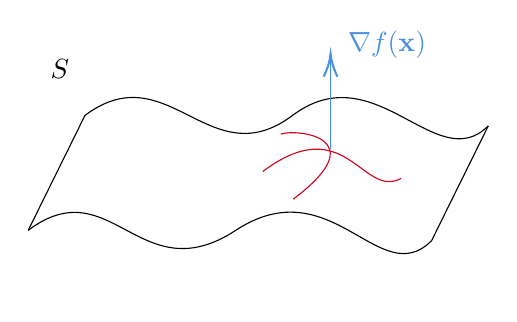
\begin{tikzpicture}[x=0.75pt,y=0.75pt,yscale=-1,xscale=1]
%uncomment if require: \path (0,300); %set diagram left start at 0, and has height of 300

%Curve Lines [id:da603117615542309] 
\draw    (182,133.33) .. controls (222,103.33) and (242,163.33) .. (282,133.33) .. controls (322,103.33) and (351.33,163.33) .. (376.33,138.33) ;
%Curve Lines [id:da030806806310122115] 
\draw    (154.67,188.67) .. controls (194.67,158.67) and (208.33,219) .. (254.67,188.67) .. controls (301,158.33) and (324,218.67) .. (349,193.67) ;
%Straight Lines [id:da891425558098866] 
\draw    (182,133.33) -- (154.67,188.67) ;
%Straight Lines [id:da3777746705205005] 
\draw    (376.33,138.33) -- (349,193.67) ;
%Curve Lines [id:da966844915291705] 
\draw [color={rgb, 255:red, 208; green, 2; blue, 27 }  ,draw opacity=1 ]   (267.67,160.33) .. controls (307.67,130.33) and (315.67,173.67) .. (334.33,163.67) ;
%Straight Lines [id:da4872470345315718] 
\draw [color={rgb, 255:red, 74; green, 144; blue, 226 }  ,draw opacity=1 ]   (300.38,149.51) -- (300.34,105.67) ;
\draw [shift={(300.33,103.67)}, rotate = 449.94] [color={rgb, 255:red, 74; green, 144; blue, 226 }  ,draw opacity=1 ][line width=0.75]    (10.93,-3.29) .. controls (6.95,-1.4) and (3.31,-0.3) .. (0,0) .. controls (3.31,0.3) and (6.95,1.4) .. (10.93,3.29)   ;
%Curve Lines [id:da2744551672083855] 
\draw [color={rgb, 255:red, 208; green, 2; blue, 27 }  ,draw opacity=1 ]   (282.33,173.67) .. controls (322.33,143.67) and (283.67,139.67) .. (276.33,142.33) ;

% Text Node
\draw (164.21,105.31) node [anchor=north west][inner sep=0.75pt]    {$S$};
% Text Node
\draw (307.54,91.31) node [anchor=north west][inner sep=0.75pt]  [color={rgb, 255:red, 74; green, 144; blue, 226 }  ,opacity=1 ]  {$\nabla f(\mathbf{x})$};


\end{tikzpicture}

 \end{center}


 \subsection{Computing Gradients}

In the example in the previous section, computing the gradient was somewhat difficult, requiring various expansions. We might wonder if it is possible to compute it more efficiently, in some orthogonal curvilinear coordinates.

In Cartesian coordinates, things are straightforward.
To get the change $\vv{x} \mapsto \vv{x} + \vv{h}$, we could just get the change $x \mapsto x + h_1$, $y \mapsto y + h_2$, $z \mapsto z + h_3$, then
\begin{align*}
f(\vv{x} + \vv{h}) &= f(x + h_1, y + h_2, z + h_3) \\
				   &= f(\vv{x}) + \frac{\partial f}{\partial x} h_1 + \frac{\partial f}{\partial y} h_2  + \frac{\partial f}{\partial z} h_3 + o(\vv{h}) \\
				   &= f(\vv{x}) +  \begin{pmatrix}
					\partial f / \partial x \\
					\partial f / \partial y \\
					\partial f / \partial z 
				   \end{pmatrix} \cdot \vv{h} + o(\vv{h}),
\end{align*}
so
$$
\nabla f = \begin{pmatrix}
	\partial f / \partial x \\
	\partial f / \partial y \\
	\partial f / \partial z 
   \end{pmatrix}.
$$
Or, using suffix notation, 
$$
\nabla f = \vv{e}_i \frac{\partial f}{\partial x_i}, \quad \text{or} \quad [\nabla f]_i = \frac{\partial f}{\partial x_i}.
$$
We can see that $\nabla$ is a kind of vector differential operator.

So let's try and see how to apply this to other coordinate systems. Recall that in Cartesian coordinates, the line element was
$$
\dd \vv x = \dd x \vv{e}_x + \dd y \vv{e}_y + \dd z \vv{e}_z = \dd x_i \vv{e}_i.
$$
Also a function $f = f(x, y, z)$ has differential
$$
\dd f = \frac{\partial f}{\partial x_i} \dd x_i.
$$
Then
\begin{align*}
	\nabla f \cdot \dd \vv{x} &= \left(\vv{e}_i \frac{\partial f}{\partial x_i}\right) \cdot (\vv{e}_j \dd x_j) \\
	&= \frac{\partial f}{\partial x_i} \underbrace{\vv{e}_i \cdot \vv{e}_j}_{\delta_{ij}} \; \dd x_j \\
	&= \frac{\partial f}{\partial x_i} \dd x_i \\
	&= \dd f.
\end{align*}
So we have the following important result:
$$
\boxed{\nabla f \cdot \dd \vv{x} = \dd f}
$$
This result is important because it is \emph{coordinate independent}.

\begin{remark}[Abuse of Notation]
	So far we have jumped from writing $f(\vv{x}) \rightarrow f(x, y, z)$. Really, what we should have written is $F(x, y, z) = f(\vv{x}(x, y, z))$. This seems over the top in Cartesian coordinates, but would be far more proper to write $F(u, v, w) = f(\vv{x}(u, v, w))$.
\end{remark}

\begin{proposition}
	If $(u, v, w)$ are orthogonal curvilinear coordinates and $f = f(u, v, w)$, then
	$$
	\nabla f = \frac{1}{h_u} \frac{\partial f}{\partial u} \vv{e}_u + \frac{1}{h_v} \frac{\partial f}{\partial v} \vv{e}_v + \frac{1}{h_w} \frac{\partial f}{\partial w} \vv{e}_w.
	$$
\end{proposition}
\begin{proof}
	If $f = f(u, v, w)$ and $\vv{x} = \vv{x}(u, v, w)$, then
	$$
\dd f = \frac{\partial f}{\partial u} \dd u + \frac{\partial f}{\partial v} \dd v + \frac{\partial f}{\partial w} \dd w,
	$$
	and
	$$
	\dd \vv{x} = h_u \dd u \vv{e}_u + h_v \dd v \vv{e}_v + h_w \dd w \vv{e}_w.
	$$
	Using $\dd f = \nabla f \cdot \dd \vv{x}$,  and writing
	$$
	\nabla f = [\nabla f]_u \vv{e}_u + [\nabla f]_v \vv{e}_v + [\nabla f]_w \vv{e}_w,
	$$
	we find that
	$$
	\frac{\partial f}{\partial u} \dd u + \frac{\partial f}{\partial v} \dd v + \frac{\partial f}{\partial w} \dd w = h_u [\nabla f]_u \dd u + h_v [\nabla f]_v \dd v + h_w [\nabla f]_w \dd w.
	$$
	Since $\{\dd u, \dd v, \dd w\}$ are linearly independent, we can compare components, and we get 
	$$
	[\nabla f]_u = \frac{1}{h_u} \frac{\partial f}{\partial u},
	 \quad [\nabla f]_v = \frac{1}{h_v} \frac{\partial f}{\partial v}, 
	\quad [\nabla f]_w = \frac{1}{h_w} \frac{\partial f}{\partial w},
	$$
	as required.
\end{proof}

\begin{example}[Gradient in Cylindrical/Spherical Coordinates]
	In cylindrical polar coordinates $(\rho, \phi, z)$, we have $h_\rho = 1$, $h_\phi = \rho$, and $h_z = 1$. So
	$$
	\nabla f = \frac{\partial f}{\partial \rho} \vv{e}_\rho + \frac{1}{\rho}\frac{\partial f}{\partial \phi} \vv{e}_\phi + \frac{\partial f}{\partial z} \vv{e}_z.
	$$

	In spherical polar coordinates $(r, \theta, \phi)$, we have $h_r = 1$, $h_\theta = r$ and $h_\phi = r \sin \theta$. Then
	$$
\nabla f = \frac{\partial f}{\partial r} \vv{e}_r + \frac{1}{r} \frac{\partial f}{\partial \theta} \vv{e}_\theta + \frac{1}{ r \sin \theta} \frac{\partial f}{\partial \phi} \vv{e}_\phi.
	$$
\end{example}

\section{Integration over Lines, Surfaces and Volumes}

We are now going to move on to the other (possibly more interesting) side of Calculus -- integration! We are going to study how integration can be performed over various objects, beginning with lines (a rather simple generalization of `normal' integration), followed by surfaces and volumes.

\subsection{Line Integrals}

We will begin by defining the line integral.

\begin{definition}[Line Integral]
	For a vector field $\vv{F} = \vv{F}(\vv{x})$ and a piecewise smooth parameterized curve $t \mapsto \vv{x}(t)$ with $t \in [a, b]$, we define the \vocab{line integral}
	$$
	\int_C \vv{F} \cdot \dd \vv{x} = \int_a^b \vv{F}(\vv{x}(t)) \cdot \frac{\dd \vv{x}}{\dd t} \dd t.
 	$$
\end{definition}

Note that the direction is important (we integrate over `increasing $t$'). If we wanted to integrate in the opposite direction over the curve, we would consider $\int_{-C}$.

\begin{example}
	\label{ex:q}
	Consider the vector field 
	$$
	\vv{F} = \begin{pmatrix}
		x^2 y \\ yz \\ 2zx
	\end{pmatrix},
	$$
	and consider two curves connecting the origin to $(1, 1, 1)$,
	\begin{align*}
		C_1: t \longmapsto \begin{pmatrix}
			t \\ t\\ t
		\end{pmatrix}, \quad t \in [0, 1], \quad \quad
		C_2: t \longmapsto \begin{pmatrix}
			t \\ t\\ t^2
		\end{pmatrix}, \quad t \in [0, 1].
	\end{align*}
	So
	$$
	\int_{C_1} \vv{F} \cdot \dd \vv{x}= \int_0^1 \begin{pmatrix}
		t^3 \\ t^2\\ 2t^2
	\end{pmatrix} \cdot \begin{pmatrix}
		1 \\ 1\\ 1
	\end{pmatrix} \dd t = \frac{5}{4}.
	$$
	and
	$$
	\int_{C_2} \vv{F} \cdot \dd \vv{x}= \int_0^1 \begin{pmatrix}
		t^3 \\ t^2\\ 2t^2
	\end{pmatrix} \cdot \begin{pmatrix}
		1 \\ 1\\ 2t
	\end{pmatrix} \dd t = \frac{13}{10}.
	$$
\end{example}

We can see from the above example that the line integral between two points depends on the path taken.

\begin{example}
	A particle at $\vv{x}$ experiences a force in cylindrical polars of
	$$
	\vv{F}(\vv{x}) = z \rho \vv{e}_{\phi}.
	$$
	We will calculate the work done by travelling along
	$$
	C: t \longmapsto \begin{pmatrix}
		a \cos t \\ a \sin t \\ t
	\end{pmatrix}, \quad t \in [0, 2\pi].
	$$

	Recall the line element in cylindrical polars is
	$$
	\dd \vv{x} = \dd \rho \vv{e}_{\rho} + \rho \dd \phi \vv{e}_{\phi} + \dd z \vv{e}_z.
	$$
	So
	$$
\vv{F} \cdot \dd \vv{x} = z \rho^2 \dd \phi.
	$$
	Also on the path $(\rho, \phi, z) = (a, t, t)$, so $(\dd \rho, \dd \phi, \dd z) = (0, \dd t, \dd t)$. So $\vv{F} \cdot \dd \vv{x} = a^2 t \dd t$. Finally,
	$$
	\int_C \vv{F} \cdot \dd \vv{x} = a^2 \int_0^{2 \pi} t \dd t = 2 \pi^2 a^2.
	$$
\end{example}

A curve $\vv{x}(t)$ with $t \in [a, b]$ might be such that $\vv{x}(a) = \vv{x}(b)$, that is, the curve is \emph{closed}. In this case, we write
$$
\oint_C \vv{F} \cdot \dd \vv{x}.
$$
Sometimes we call integrals of this form the \vocab{circulation} of $\vv{F}$ about $C$.

\begin{example}
	Using $C_1$ and $C_2$ from \autoref{ex:q}, we define the curve $C = C_1 - C_2$. Then
	$$
		\oint_C \vv{F} \cdot \dd \vv{x} = \int_{C_1} \vv{F} \cdot \dd \vv{x} - \int_{C_2} \vv{F} \cdot \dd \vv{x} = - \frac{2}{15}.
	$$
\end{example}

\subsection{Conservative Forces and Exact Differentials}

We have seen how to interpret things like $\vv{F} \cdot \dd \vv{x}$ when they're inside an integral. This is another differential form, that is, in coordinates $(u, v, w)$,
$$
\vv{F} \cdot \dd x = (\ )\dd u + (\ ) \dd v + (\ ) \dd w,
$$
where there's \emph{something} inside the brackets.

\begin{definition}[Exactness]
	We say that $\vv{F} \cdot\dd \vv{x}$ is \vocab{exact} if
	$
	\vv{F} \cdot \dd \vv{x} = \dd f,
	$
	for some scalar function $f$.
\end{definition}

Recall that $\dd f = \nabla f \cdot \dd \vv{x}$, so $\vv{F} \cdot \dd \vv{x}$ is exact if and only if $\vv{F} = \nabla f$ for some scalar function $f$. We call such vector fields \vocab{conservative}.


For a vector field $\vv{F}$, we have $\vv{F} \cdot \dd \vv{x}$ is exact if and only if $\vv{F}$ is conservative.

Using properties such as $\dd(\alpha f + \beta g) = \alpha \dd f + \beta \dd g$ for constant $\alpha, \beta$ and $\dd(fg) = g \dd f + f \dd g$, usually it is easy to see if a differential form $\vv{F} \cdot \dd \vv{x}$ is exact.

\begin{proposition}
	If $\theta$ is an exact differential form, then
	$$
	\oint_C \theta = 0,
	$$
	for any closed curve $C$.
\end{proposition}
\begin{proof}
	If $\theta$ is exact, then $\theta = \nabla f \cdot \dd \vv{x}$ for some scalar $f$. If $C: t \mapsto \vv{x}(t)$ with $t \in [a, b]$,
	\begin{align*}
		\oint_C \theta &= \oint_C \nabla f \cdot \dd \vv{x} \\
			&= \int_{a}^b \nabla f(\vv{x}(t)) \cdot \frac{\dd \vv{x}}{\dd t} \dd t \\
			&= \int_a^b \frac{\dd}{\dd t} \left[f(\vv{x}(t))\right] \dd t \\
			&= f(\vv{x}(b)) - f(\vv{x}(a))\\
			&= 0,
	\end{align*}
	if $\vv{x}(a) = \vv{x}(b)$.
\end{proof}

Equivalently, if $\vv{F}$ is conservative, then the circulation of $\vv{F}$ around any closed loop curve $C$ vanishes,  $\oint_C \vv{F} \cdot \dd \vv{x} = 0$.

Also if $\vv{F}$ is conservative (and $\vv{F} \cdot \dd \vv{x}$ is exact), then the line integral between points $A = \vv{x}(a)$ and $B = \vv{x}(b)$ is \emph{independent} of path.

Now let $(u, v, w)$ be an arbitrary set of orthonormal curvilinear coordinates. Let
$$
\vv{F} \cdot \dd \vv x = \theta = \underbrace{A(u, v, w)}_{\theta_1} \dd u + \underbrace{B(u, v, w)}_{\theta_2} \dd v + \underbrace{C(u, v, w)}_{\theta_3} \dd w = \theta_i \dd u_i.
$$
A \emph{necessary} condition for $\theta$ to be exact is
$$
	\frac{\partial \theta_i}{\partial u_j} = \frac{\partial \theta_j}{\partial u_i}, \quad \quad \text{for each }i, j.
$$
Indeed, if $\theta$ is exact, then $\theta = \dd f$ for some $f$. Then
\begin{equation}\label{eq:closed}
	\theta = \frac{\partial f}{\partial u_i} \dd u_i \iff \theta_i = \frac{\partial f}{\partial u_i},\tag{$*$}
\end{equation}
and so
$$
	\frac{\partial \theta_i}{\partial u_j} = \frac{\partial^2 f}{\partial u_j \partial u_i} = \frac{\partial^2 f}{\partial u_i \partial u_j} = \frac{\partial \theta_j}{ \partial u_i}.
$$

If a differential form satisfies \eqref{eq:closed}, we call it \vocab{closed}. So if $\theta$ is exact, then $\theta$ is closed.

The reverse implication is true if the domain $\Omega \subset \R^3$ on which $\theta$ is defined is simply-connected\footnote{All closed loops in $\Omega$ can be `continuously shrunk' to any point inside $\Omega$ without leaving it.}. We will be able to prove this later on, using Stokes' theorem.

\begin{example}
	Consider $\theta = y \dd x - x \dd y$. We will check if it is closed. If so, we need to have
	$$
	\frac{\partial y}{\partial y} = \frac{\partial -x}{\partial x},
	$$
	which is clearly not the case, as $1 \neq -1$. Thus $\theta$ is not exact.
\end{example}

\begin{example}[Silly Example]
	We will compute the line integral
	$$
	\oint_C 3x^2 y \dd x + x^3 \dd y,
	$$
	over the curve
	$$
	C: t \mapsto \begin{pmatrix}
		\cos(\im(\zeta(1/2 + it))) \\
		\sin(\re(\zeta(1/2 + it))) \\
		0
	\end{pmatrix}, \quad \quad t \in [\alpha_1, \alpha_{100}],
	$$
	where $\alpha_1$ and $\alpha_{100}$ are the 1st and 100th zero of $\zeta(1/2 + it)$, so that $\zeta(1/2 + i \alpha_1) = \zeta(1/2 + i \alpha_{100}) = 0$.
	
	Now this differential form is exact, as $3x^2 y \dd x + x^3 \dd y = \dd (x^3 y)$, and $C$ is a closed curve (both endpoints are $(1, 0, 0)$), thus $\oint_C 3x^2 y \dd x + x^3 \dd y = 0$.
\end{example}

\subsection{Integration in $\R^2$}

We want to integrate over some bounded region say $D \subset \R^2$. To do this, we will cover $D$ with small, disjoint sets $A_{ij}$, each with area $\delta A_{ij}$, so that each of these are contained in a disk of radius $\epsilon > 0$.
Let $(x_i, y_j)$ be points contained in each $A_{ij}$.

Now define
$$
	\int_D f(\vv{x}) \dd A = \lim_{\epsilon \to 0} \sum_{i,j} f(x_i, y_j) \delta A_{ij}
$$
We will say that the integral exists if it is independent of our choice of $A_{ij}$ and choice of $(x_i, y_j)$.

An obvious choice of partition would be to use rectangles with $\delta A_{ij} = \delta x \delta y$. We could sum over horizontal strips of width $\delta y$, then take the limit as $\delta x \rightarrow 0$. This gives
$$
	\delta y \int_{X_y} f(x, y) \dd x,
$$
where $X_y = \{x \mid (x, y) \in D \}$. Summing over each such strip, we'd end up with
$$
\int_{D} f(x, y) \dd A = \int_Y \left(\int_{X_y} f(x, y) \dd x\right) \dd y,
$$
where $Y$ is as in the diagram below.

\begin{center}
	

\tikzset{every picture/.style={line width=0.75pt}} %set default line width to 0.75pt        

\begin{tikzpicture}[x=0.75pt,y=0.75pt,yscale=-1,xscale=1]
%uncomment if require: \path (0,300); %set diagram left start at 0, and has height of 300

%Straight Lines [id:da1629034885697126] 
\draw    (200,210) -- (418,210) ;
\draw [shift={(420,210)}, rotate = 180] [color={rgb, 255:red, 0; green, 0; blue, 0 }  ][line width=0.75]    (10.93,-3.29) .. controls (6.95,-1.4) and (3.31,-0.3) .. (0,0) .. controls (3.31,0.3) and (6.95,1.4) .. (10.93,3.29)   ;
%Straight Lines [id:da31151739933589306] 
\draw    (210,220) -- (210,22) ;
\draw [shift={(210,20)}, rotate = 450] [color={rgb, 255:red, 0; green, 0; blue, 0 }  ][line width=0.75]    (10.93,-3.29) .. controls (6.95,-1.4) and (3.31,-0.3) .. (0,0) .. controls (3.31,0.3) and (6.95,1.4) .. (10.93,3.29)   ;
%Shape: Polygon Curved [id:ds10249847549557578] 
\draw   (250,90) .. controls (270,80) and (360,70) .. (340,90) .. controls (320,110) and (320,120) .. (340,150) .. controls (360,180) and (270,180) .. (250,150) .. controls (230,120) and (230,100) .. (250,90) -- cycle ;
%Straight Lines [id:da25451399177896894] 
\draw  [dash pattern={on 0.84pt off 2.51pt}]  (321,78) -- (210,78) ;
%Straight Lines [id:da041739869365173266] 
\draw  [dash pattern={on 0.84pt off 2.51pt}]  (309,173) -- (210,173) ;
%Shape: Brace [id:dp6621245674606429] 
\draw   (210,78.75) .. controls (205.33,78.72) and (202.99,81.04) .. (202.96,85.71) -- (202.81,115.71) .. controls (202.77,122.38) and (200.42,125.7) .. (195.75,125.68) .. controls (200.42,125.7) and (202.73,129.04) .. (202.7,135.71)(202.72,132.71) -- (202.54,165.71) .. controls (202.52,170.38) and (204.84,172.72) .. (209.51,172.75) ;
%Straight Lines [id:da07321232057182314] 
\draw [color={rgb, 255:red, 208; green, 2; blue, 27 }  ,draw opacity=1 ]   (239,130) -- (328,130) ;
%Straight Lines [id:da3528968860450654] 
\draw [color={rgb, 255:red, 208; green, 2; blue, 27 }  ,draw opacity=1 ]   (237,124) -- (326,124) ;
%Straight Lines [id:da29786796871231136] 
\draw    (380,130) -- (331,127.12) ;
\draw [shift={(329,127)}, rotate = 363.37] [color={rgb, 255:red, 0; green, 0; blue, 0 }  ][line width=0.75]    (10.93,-3.29) .. controls (6.95,-1.4) and (3.31,-0.3) .. (0,0) .. controls (3.31,0.3) and (6.95,1.4) .. (10.93,3.29)   ;
%Straight Lines [id:da30084043292662677] 
\draw  [dash pattern={on 4.5pt off 4.5pt}]  (239,130) -- (239,210) ;
%Straight Lines [id:da7980958464242905] 
\draw  [dash pattern={on 4.5pt off 4.5pt}]  (328,130) -- (328,210) ;
%Shape: Brace [id:dp5081444039097228] 
\draw   (239,210.75) .. controls (239.03,215.42) and (241.37,217.74) .. (246.04,217.71) -- (273.29,217.56) .. controls (279.96,217.52) and (283.3,219.83) .. (283.33,224.5) .. controls (283.3,219.83) and (286.62,217.48) .. (293.29,217.45)(290.29,217.46) -- (320.54,217.29) .. controls (325.21,217.27) and (327.53,214.93) .. (327.5,210.26) ;

% Text Node
\draw (351,63) node [anchor=north west][inner sep=0.75pt]    {$D$};
% Text Node
\draw (181,122) node [anchor=north west][inner sep=0.75pt]    {$Y$};
% Text Node
\draw (382,130) node [anchor=west] [inner sep=0.75pt]    {$\delta y$};
% Text Node
\draw (271,232) node [anchor=north west][inner sep=0.75pt]    {$X_{y}$};


\end{tikzpicture}

\end{center}

If we instead sum over vertical strips, we get 
$$
	\int_D f(x, y) \dd A = \int_X \left(\int_{Y_x} f(x, y) \dd y\right) \dd x.
$$

More concisely, we have
$$
\dd A = \dd x \dd y = \dd y \dd x. 
$$
This is known as Fubini's theorem (with a few caveats that we won't worry about), which you may meet properly in a later course.

\begin{example}
	Let $D$ be a triangle with vertices at $(0, 0)$, $(1, 0)$ and $(0, 1)$. 

	\begin{center}
		

\tikzset{every picture/.style={line width=0.75pt}} %set default line width to 0.75pt        

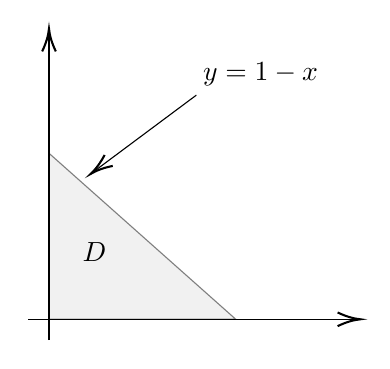
\begin{tikzpicture}[x=0.75pt,y=0.75pt,yscale=-1,xscale=1]
%uncomment if require: \path (0,300); %set diagram left start at 0, and has height of 300

%Shape: Right Triangle [id:dp07296511159724295] 
\draw  [color={rgb, 255:red, 128; green, 128; blue, 128 }  ,draw opacity=1 ][fill={rgb, 255:red, 241; green, 241; blue, 241 }  ,fill opacity=1 ] (210,130) -- (300,210) -- (210,210) -- cycle ;
%Straight Lines [id:da19925281886663593] 
\draw    (200,210) -- (358,210) ;
\draw [shift={(360,210)}, rotate = 180] [color={rgb, 255:red, 0; green, 0; blue, 0 }  ][line width=0.75]    (10.93,-3.29) .. controls (6.95,-1.4) and (3.31,-0.3) .. (0,0) .. controls (3.31,0.3) and (6.95,1.4) .. (10.93,3.29)   ;
%Straight Lines [id:da9848620958169408] 
\draw    (210,220) -- (210,72) ;
\draw [shift={(210,70)}, rotate = 450] [color={rgb, 255:red, 0; green, 0; blue, 0 }  ][line width=0.75]    (10.93,-3.29) .. controls (6.95,-1.4) and (3.31,-0.3) .. (0,0) .. controls (3.31,0.3) and (6.95,1.4) .. (10.93,3.29)   ;
%Straight Lines [id:da6104098831517629] 
\draw    (281,102) -- (231.6,138.81) ;
\draw [shift={(230,140)}, rotate = 323.31] [color={rgb, 255:red, 0; green, 0; blue, 0 }  ][line width=0.75]    (10.93,-3.29) .. controls (6.95,-1.4) and (3.31,-0.3) .. (0,0) .. controls (3.31,0.3) and (6.95,1.4) .. (10.93,3.29)   ;

% Text Node
\draw (225,172) node [anchor=north west][inner sep=0.75pt]    {$D$};
% Text Node
\draw (283,99) node [anchor=south west] [inner sep=0.75pt]    {$y=1-x$};


\end{tikzpicture}

	\end{center}
	If $f(x, y) = xy^2$, then if we integrate over horizontal strips, 
	\begin{align*}
		\int_D f \dd A &= \int_0^1\left(\int_{0}^{1 - y} xy^2 \dd x \right) \dd y\\
	&= \int_0^1 y^2 \left[ \frac{1}{2}x^2 \right]_0^{1 - y} \dd y \\
	&= \int_0^1 \frac{1}{2} y^2 (1 - y)^2 \dd y = \frac{1}{60}.
	\end{align*}
	If we did the same with vertical strips, we could get
	\begin{align*}
		\int_D f \dd A &= \int_0^1 \left(\int_0^{1 - x} xy^2 \dd y\right) \dd x \\
		&= \int_0^1 x \left[\frac{1}{3}y^3\right]_0^{1 - x} \dd x = \frac{1}{60},
	\end{align*}
	and they are the same.
\end{example}

A special case is when $f(x, y) = g(x)h(y)$ and $D$ is a rectangle, $D = \{(x, y) \mid a \leq x \leq b, c \leq y \leq d \}$, then
$$
\int_D f(x, y) \dd A = \left(\int_{a}^b g(x) \dd x\right)\left(\int_c^d h(y) \dd y\right).
$$

It is often useful to introduce a change of variables to compute $\int_a^b f(x) \dd x$.
If we introduce $x = x(u)$ with $x(\alpha) = a$ and $x(\beta) = b$, then
$$
\int_a^b f(x)\dd x = \begin{cases}
	+ \int_\alpha^\beta f(x(u)) \frac{\dd x}{\dd u} \dd u &\mbox{if } \beta > \alpha, \\
	- \int_\beta^\alpha f(x(u)) \frac{\dd x}{\dd u} \dd u  &\mbox{if } \alpha > \beta.
   \end{cases}
$$
So if $I = [a, b]$ is the image under $x$ of an interval $I'$, then
$$
\int_I f(x) \dd x = \int_{I'} f(x(u)) \left|\frac{\dd x}{\dd u}\right| \dd u.
$$

There is a similar formula in two dimensions.

\begin{proposition}
	Let $x = x(u, v)$ and $y = y(u, v)$ be a smooth, invertible transformation with smooth inverse that maps the region $D'$ in the $(u, v)$ plane to the region $D$ in the $(x, y)$-plane.
	Then
	$$
	\int_D f(x, y) \dd x \dd y = \int_{D'} f(x(u, v), y(u, v)) \left|\frac{\partial(x, y)}{\partial(u, v)}\right| \dd u \dd v,
	$$
	where
	$$
	\frac{\partial (x, y)}{\partial (u, v)} = \det\begin{pmatrix}
		\partial x/\partial u & \partial x / \partial v \\
		\partial y / \partial u & \partial y / \partial v
	\end{pmatrix}
	$$
	is the \emph{Jacobian}, often denoted by $J$.
\end{proposition}

The short version is that $\dd x \dd y = |J| \dd u \dd v$.

\begin{example}
	Using polar coordinates $(\rho, \phi)$,
	$$
	x(\rho, \phi) = \rho \cos \phi, \quad \quad y(\rho, \phi) = \rho \sin \phi.
	$$
	Hence 
	$$
	J = \det \begin{pmatrix}
		\cos \phi & - \rho \sin \phi \\
		\sin \phi & \rho \cos \phi
	\end{pmatrix} = \rho,
	$$
	So if $D = \{(x, y)  \mid x > 0, y > 0, x^2 + y^2 < R^2 \}$, then $D' = \{(\rho, \phi) \mid 0 < \rho < R, 0 < \phi < \pi/2\}$, and
	$$
	\int_D f(x, y) \dd x\ \dd y = \int_{D'} f(\rho \cos \phi, \rho \sin \phi) \rho\  \dd \rho \dd \phi,
	$$
	so $\dd x \dd y = \rho \dd \rho \dd \phi$.

	Taking $R \rightarrow \infty$, we get
	$$
	\int_{x = 0}^{\infty} \int_{y = 0}^{\infty} f(x, y) \dd y \dd x = \int_{\phi = 0}^{\pi/2} \int_{\rho = 0}^{\infty} f(\rho \cos \phi, \rho \sin \phi) \rho \; \dd \rho \dd\phi.
	$$

	Now consider $I = \int_0^{\infty} e^{-x^2} \dd x$. Using the previous result, we have
	\begin{align*}
		I^2 &= \int_{0}^{\infty} e^{-x^{2}} \dd x \cdot \int_{0}^{\infty} e^{-y^{2}} \dd y \\
			&= \int_{x=0}^{\infty} \int_{y=0}^{\infty} e^{-x^{2}-y^{2}} \dd x \dd y \\
			&= \int_{\phi = 0}^{\pi/2} \left(\int_{\rho = 0}^{\infty} e^{- \rho^2} \rho \dd\rho \right) \dd \phi \\
			&= \frac{\pi}{2} \int_0^{\infty} \frac{\dd}{\dd \rho} \left(-\frac{1}{2} e^{- \rho^2}\right) \dd \rho = \frac{\pi}{4}.
	\end{align*}
	Thus $I = \frac{\sqrt{\pi}}{2}$.
\end{example}

\subsection{Integration in $\R^3$}

To integrate over a region $V$ in $\R^3$, we use similar ideas to that of the previous section. Let
$$
	\int_V f(\vv{x}) \dd V = \lim_{\epsilon \to 0} \sum_{i, j, k} f(x_i, y_j, z_k) \delta V_{ijk},
$$
where the \emph{volume element} satisfies
$$
\dd V = \dd x \ \dd y \ \dd z.
$$
We can do the integrals in any order (again Fubini's theorem).

\begin{example}
	Consider the region $V$ bound by planes $x + y + z = 1$ and $x = 0, y = 0$ and $z = 0$. We will find the volume (integrating $1$ over the region).
	\begin{center}
		

\tikzset{every picture/.style={line width=0.75pt}} %set default line width to 0.75pt        

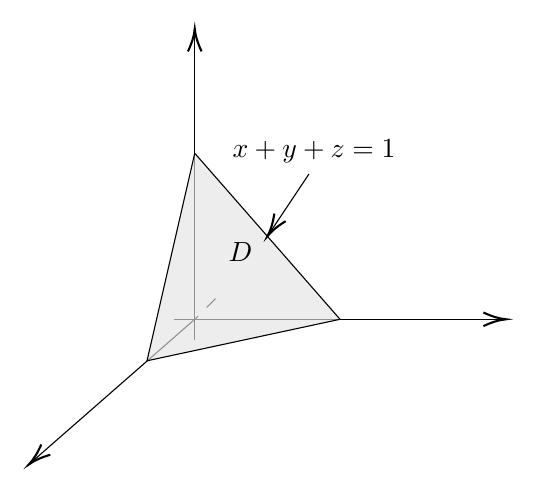
\begin{tikzpicture}[x=0.75pt,y=0.75pt,yscale=-1,xscale=1]
%uncomment if require: \path (0,300); %set diagram left start at 0, and has height of 300

%Straight Lines [id:da7142734641721928] 
\draw    (200,210) -- (358,210) ;
\draw [shift={(360,210)}, rotate = 180] [color={rgb, 255:red, 0; green, 0; blue, 0 }  ][line width=0.75]    (10.93,-3.29) .. controls (6.95,-1.4) and (3.31,-0.3) .. (0,0) .. controls (3.31,0.3) and (6.95,1.4) .. (10.93,3.29)   ;
%Straight Lines [id:da7321899041114295] 
\draw    (210,220) -- (210,72) ;
\draw [shift={(210,70)}, rotate = 450] [color={rgb, 255:red, 0; green, 0; blue, 0 }  ][line width=0.75]    (10.93,-3.29) .. controls (6.95,-1.4) and (3.31,-0.3) .. (0,0) .. controls (3.31,0.3) and (6.95,1.4) .. (10.93,3.29)   ;
%Straight Lines [id:da3568532467086144] 
\draw    (210,210) -- (131.51,278.68) ;
\draw [shift={(130,280)}, rotate = 318.81] [color={rgb, 255:red, 0; green, 0; blue, 0 }  ][line width=0.75]    (10.93,-3.29) .. controls (6.95,-1.4) and (3.31,-0.3) .. (0,0) .. controls (3.31,0.3) and (6.95,1.4) .. (10.93,3.29)   ;
%Straight Lines [id:da2728884008736586] 
\draw  [dash pattern={on 4.5pt off 4.5pt}]  (220,200) -- (210,210) ;
%Shape: Polygon [id:ds4065449031533396] 
\draw  [fill={rgb, 255:red, 227; green, 227; blue, 227 }  ,fill opacity=0.64 ] (280,210) -- (187,230) -- (210,130) -- cycle ;
%Straight Lines [id:da8133123312139356] 
\draw    (265,140) -- (246.11,168.34) ;
\draw [shift={(245,170)}, rotate = 303.69] [color={rgb, 255:red, 0; green, 0; blue, 0 }  ][line width=0.75]    (10.93,-3.29) .. controls (6.95,-1.4) and (3.31,-0.3) .. (0,0) .. controls (3.31,0.3) and (6.95,1.4) .. (10.93,3.29)   ;

% Text Node
\draw (225,172) node [anchor=north west][inner sep=0.75pt]    {$D$};
% Text Node
\draw (227,122) node [anchor=north west][inner sep=0.75pt]    {$x+y+z=1$};


\end{tikzpicture}

	\end{center} 
We have
\begin{align*}
	\int_V \dd V &= \int_{x = 0}^1 \left(\int_{y = 0}^{1 - x} \left(\int_{z = 0}^{1 - x - y} \dd z\right) \dd y\right) \dd x \\
	&= \int_{x = 0}^{1} \int_{y = 0}^{1 - x}(1 - x - y) \dd y \dd x \\
	&= \frac{1}{6}.
\end{align*}

If we wanted to compute say the center of mass, then assuming it had constant density say $\rho = 1$, the centre of mass $\vv{X}$ is
$$
\vv{X} = \frac{1}{M} \int_V \rho \vv{x} \dd V = \frac{1}{4}\begin{pmatrix}
	1\\ 1\\ 1
\end{pmatrix}
$$
\end{example}

We can write down the change of variables for three dimensional integrals.

\begin{proposition}
	Let $x = x(u, v, w)$, $y = y(u, v, w)$ and $z = z(u, v, w)$ be a continuously differentiable bijection with continuously differentiable inverse that maps the volume $V'$ to $V$. Then
	$$
	\int_V f(x, y, z) \dd x \ \dd y \ \dd z = \int_{V'} f(x(u, v, w), y(u, v, w), z(u, v, w)) |J| \dd u\  \dd v\ \dd w,
	$$
	where
	$$
	J = \frac{\partial(x, y, z)}{\partial(u, v, w)}
	$$
\end{proposition}
Again the short version is $\dd x\ \dd y\ \dd z = |J| \dd u\ \dd v\ \dd w$.

\begin{example}
	In cylindrical polars $(u, v, w) = (\rho, \phi, z)$,
	$$
	\dd V = \rho \; \dd\rho \; \dd \phi \; \dd z,
	$$
	and $|J| = \rho$.

	In spherical polars $(u, v, w) = (r, \theta, \phi)$,
	$$
	\dd V = r^2 \sin \theta \; \dd r \; \dd \theta \; \dd \phi,
	$$
	and $|J| = r^2 \sin \theta$.
\end{example}

\begin{example}
	Suppose we wanted to calculate the volume of the ball of radius $R$, $V = \{(x, y, z) \mid x^2 + y^2 + z^2 \leq R^2\}$. 
	
	We could try a `bare hands' approach in Cartesian coordinates.
	\begin{align*}
		&\ \int_V \dd V\\ &= \int_{z=-R}^{R} \left(\int_{y = - \sqrt{R^2 - z^2}}^{\sqrt{R^2 - z^2}} \left( \int_{x = - \sqrt{R^2 - z^2 - y^2}}^{\sqrt{R^2 - z^2 - y^2}} \dd x\right)\dd y\right)\dd z \\
		&=\int_{z=-R}^{R}\left[\int_{y=-\sqrt{R^{2}-z^{2}}}^{\sqrt{R^{2}-z^{2}}} 2 \sqrt{R^{2}-z^{2}-y^{2}}\; \dd y\right] \;\dd z\\
		&= \int_{z = -R}^{R}\left[y \sqrt{R^2 - z^2 - y^2} + (R^2 - z^2)\tan^{-1}\left(\frac{y}{\sqrt{R^2 - z^2 - y^2}}\right)\right]_{-\sqrt{R^2 - z^2}}^{\sqrt{R^2 - z^2}} \dd z \\
		&= \int_{-R}^R \pi (R^2 - z^2) \dd z = \frac{4 \pi R^3}{3}.
	\end{align*}

	Alternatively, since we have even a limited amount of self respect, we can use spherical polars. We have $V' = \{(r, \theta, \phi) \mid 0 \leq r \leq R, 0 \leq \theta \leq \pi, 0 \leq \phi < 2\pi\}$. Then
	\begin{align*}
		\int_V \dd V &= \int_{\phi=0}^{2 \pi}\left[\int_{\theta=0}^{\pi}\left[\int_{r=0}^{R} r^{2} \sin \theta \; \dd r\right] \dd \theta\right] \dd \phi \\
		&= \int_{\theta=0}^{\pi} \frac{2 \pi R^{3}}{3} \sin \theta \dd\theta = \frac{4 \pi R^3}{3}.
	\end{align*}
	And this is clearly much nicer.
\end{example}

\begin{example}
	Consider a ball of radius $a$ with a cylinder of radius $b < a$ removed. The symmetry suggests that we use cylindrical polar coordinates. In Cartesian coordinates, we would have
	$$
	V = \{(x, y, z) \mid x^2 + y^2 + z^2 \leq a^2, x^2 + y^2 \geq b^2 \},
	$$
	but in cylindrical polars we would have
	$$
	V' = \{(\rho, \phi, z) \mid b \leq \rho \leq a, 0 \leq z^2 + \rho^2 \leq a^2, 0 \leq \phi < 2 \pi\}.
	$$
	So we have
	\begin{align*}
		\int_V \dd V &= \int_{\rho=b}^a \left[\int_{\phi = 0}^{2\pi}\left[\int_{z = -\sqrt{a^2 - \rho^2}}^{\sqrt{a^2 - \rho^2}}\dd z\right]\dd \phi\right]\rho \dd \rho \\
		&= 2 \pi \int_{b}^a 2\rho\sqrt{a^2 - \rho^2} \dd \rho \\
		&= \frac{4 \pi}{3}(a^2 - b^2)^{3/2}.
	\end{align*}
\end{example}

\subsection{Integration Over Surfaces}

We have now integrated over curves, over regions of the plane, and over volumes. The remaining object to integrate over is a \emph{surface} in $\R^3$, and this is where things get interesting -- surface integrals are the key ingredient in the integral theorems that we are building towards.

\subsubsection{Surfaces and Their Boundaries}

A two dimensional surface in $\R^3$ can be defined \emph{implicitly} using a function $f : \R^3 \rightarrow \R$, by setting
$$
S = \{\vv{x} \in \R^3 \mid f(\vv{x}) = 0\}.
$$
We saw before that $\nabla f$ is normal to the level sets of $f$, so the normal to $S$ at $\vv{x}$ is parallel to $\nabla f(\vv{x})$. In analogy with what we did for curves, we say the surface is \vocab{regular} if $\nabla f(\vv{x}) \neq \vv{0}$ on $S$, which rules out any `spikes' or `creases'.

\begin{example}[The Sphere]
	Take $f(\vv{x}) = x^2 + y^2 + z^2 - 1$, so that
	$$
	S = \{(x, y, z) \mid x^2 + y^2 + z^2 - 1 = 0\}
	$$
	is the unit sphere. Then $\nabla f = 2 \vv{x}$, which is never zero on $S$, and is indeed normal to the sphere at $\vv{x}$.
\end{example}

Some surfaces have a \vocab{boundary}, which we write as $\partial S$. For example, the hemisphere
$$
S = \{(x, y, z) \mid x^2 + y^2 + z^2 = 1, z \geq 0\}
$$
has boundary the circle
$$
\partial S = \{(x, y, z) \mid x^2 + y^2 = 1, z = 0\}.
$$
In this course, a surface will either have no boundary at all, or its boundary will be made up of piecewise smooth curves. If $S$ has no boundary (like the sphere), we say that $S$ is a \vocab{closed} surface.

Just as it was useful to parameterize curves, it is useful to parameterize surfaces. We do this using \emph{two} coordinates $(u, v)$, writing
$$
S = \{\vv{x} = \vv{x}(u, v) \mid (u, v) \in D\},
$$
where $D$ is some region in the $(u, v)$-plane.

\begin{example}[Parameterizing the Hemisphere]
	For the upper unit hemisphere we can use the angles from spherical polar coordinates as our parameters, writing
	$$
	S = \left\{\vv{x}(\theta, \phi) = \begin{pmatrix}
		\sin \theta \cos \phi \\
		\sin \theta \sin \phi \\
		\cos \theta
	\end{pmatrix} \;\middle|\; 0 \leq \theta \leq \frac{\pi}{2}, \; 0 \leq \phi < 2 \pi\right\}.
	$$
\end{example}

Holding $v$ fixed and varying $u$ traces out a curve in $S$ with tangent vector $\partial \vv{x}/\partial u$, and similarly for $v$. So $\partial \vv{x} / \partial u$ and $\partial \vv{x}/\partial v$ are both tangent to $S$, and (provided they are linearly independent) their cross product is \emph{normal} to $S$. With this in mind, we say the parameterization is \vocab{regular} if
$$
\frac{\partial \vv{x}}{\partial u} \times \frac{\partial \vv{x}}{\partial v} \neq \vv{0}
$$
for all $(u, v) \in D$, and in that case we obtain a unit normal
$$
\vv{n} = \frac{\frac{\partial \vv{x}}{\partial u} \times \frac{\partial \vv{x}}{\partial v}}{\left|\frac{\partial \vv{x}}{\partial u} \times \frac{\partial \vv{x}}{\partial v}\right|},
$$
which varies smoothly over the (smooth parts of the) surface.

Of course, $-\vv{n}$ is also a perfectly good unit normal, so there is a choice to be made here. A surface for which a consistent choice of unit normal can be made over all of $S$ is called \vocab{orientable}, and the choice of normal is an \vocab{orientation}\footnote{Not every surface is orientable -- the M\"obius band famously has only one side, and if you slide a normal vector all the way around the band it comes back pointing the other way. We will only work with orientable surfaces in this course.}.

An orientation of $S$ also induces an orientation on the boundary curve $\partial S$: we make the convention that $\partial S$ is traversed so that the normal vectors near the boundary point out of your \emph{left-hand side} as you walk along it. Equivalently, this is the `right-hand rule': if the thumb of your right hand points along $\vv{n}$, your fingers curl in the direction of $\partial S$.

\subsubsection{The Area Element}

Now let's integrate. Take a regular parameterized surface $S = \{\vv{x}(u, v) \mid (u, v) \in D\}$. We might naively try to define the integral of $f$ over $S$ as the integral of $f(\vv{x}(u, v))$ over the region $D$, but this can't be right -- a small patch of area $\delta u \, \delta v$ in $D$ does not generally correspond to a patch of the same area on $S$, and different parameterizations would give different answers.

Instead, let's see what a small patch actually looks like. Perturbing the coordinates one at a time,
\begin{align*}
	\vv{x}(u + \delta u, v) - \vv{x}(u, v) &= \frac{\partial \vv{x}}{\partial u} \delta u + o(\delta u), \\
	\vv{x}(u, v + \delta v) - \vv{x}(u, v) &= \frac{\partial \vv{x}}{\partial v} \delta v + o(\delta v).
\end{align*}
So to first order, the small rectangle $[u, u + \delta u] \times [v, v + \delta v]$ in $D$ is mapped to a small \emph{parallelogram} on $S$ spanned by the vectors $\frac{\partial \vv{x}}{\partial u} \delta u$ and $\frac{\partial \vv{x}}{\partial v} \delta v$. Recalling from `Vectors \& Matrices' that the area of a parallelogram is the magnitude of the cross product of its sides, this patch has area
$$
\left|\frac{\partial \vv{x}}{\partial u} \times \frac{\partial \vv{x}}{\partial v}\right| \delta u \, \delta v.
$$
This tells us exactly what the correct `scaling factor' is, and we make the following definition.

\begin{definition}[Surface Integral]
	Let $S = \{\vv{x}(u, v) \mid (u, v) \in D\}$ be a regular parameterized surface. The \vocab{scalar area element} on $S$ is
	$$
	\dd S = \left|\frac{\partial \vv{x}}{\partial u} \times \frac{\partial \vv{x}}{\partial v}\right| \dd u \dd v,
	$$
	and for $f : \R^3 \rightarrow \R$ we define
	$$
	\int_S f(\vv{x}) \dd S = \int_D f(\vv{x}(u, v)) \left|\frac{\partial \vv{x}}{\partial u} \times \frac{\partial \vv{x}}{\partial v}\right| \dd u \dd v.
	$$
\end{definition}

In particular, taking $f = 1$ gives the \emph{area} of the surface $S$.

\begin{example}[Area of a Hemisphere]
	Let $S$ be the hemisphere of radius $R$, parameterized by
	$$
	\vv{x}(\theta, \phi) = \begin{pmatrix}
		R \sin \theta \cos \phi \\
		R \sin \theta \sin \phi \\
		R \cos \theta
	\end{pmatrix} = R \vv{e}_r, \quad \quad 0 \leq \theta \leq \frac{\pi}{2}, \; 0 \leq \phi < 2\pi.
	$$
	Differentiating (or just recalling the scale factors for spherical polars),
	$$
	\frac{\partial \vv{x}}{\partial \theta} = R \vv{e}_\theta, \quad \quad \frac{\partial \vv{x}}{\partial \phi} = R \sin \theta \, \vv{e}_\phi,
	$$
	and since $\vv{e}_\theta \times \vv{e}_\phi = \vv{e}_r$ is a unit vector,
	$$
	\dd S = R^2 \sin \theta \dd \theta \dd \phi.
	$$
	The area of the hemisphere is then
	$$
	\int_S \dd S = \int_{\phi = 0}^{2 \pi} \int_{\theta = 0}^{\pi/2} R^2 \sin \theta \dd \theta \dd \phi = 2 \pi R^2,
	$$
	as expected.
\end{example}

As with curves, we should pause and check that our definition doesn't depend on the parameterization we happened to pick.

\begin{proposition}
	The integral $\int_S f(\vv{x}) \dd S$ is independent of the (regular) parameterization of $S$ used.
\end{proposition}
\begin{proof}
	Suppose $\vv{x} = \vv{x}(u, v)$ for $(u, v) \in D$ and $\vv{x} = \tilde{\vv{x}}(\tilde{u}, \tilde{v})$ for $(\tilde{u}, \tilde{v}) \in \tilde{D}$ are two parameterizations of $S$. Then there is a relationship between the coordinates, $\vv{x}(u, v) = \tilde{\vv{x}}(\tilde{u}(u, v), \tilde{v}(u, v))$, and by the chain rule
	\begin{align*}
		\frac{\partial \vv{x}}{\partial u} \times \frac{\partial \vv{x}}{\partial v} &= \left(\frac{\partial \tilde{\vv{x}}}{\partial \tilde{u}}\frac{\partial \tilde{u}}{\partial u} + \frac{\partial \tilde{\vv{x}}}{\partial \tilde{v}}\frac{\partial \tilde{v}}{\partial u}\right) \times \left(\frac{\partial \tilde{\vv{x}}}{\partial \tilde{u}}\frac{\partial \tilde{u}}{\partial v} + \frac{\partial \tilde{\vv{x}}}{\partial \tilde{v}}\frac{\partial \tilde{v}}{\partial v}\right) \\
		&= \left(\frac{\partial \tilde{u}}{\partial u} \frac{\partial \tilde{v}}{\partial v} - \frac{\partial \tilde{u}}{\partial v} \frac{\partial \tilde{v}}{\partial u}\right) \left(\frac{\partial \tilde{\vv{x}}}{\partial \tilde{u}} \times \frac{\partial \tilde{\vv{x}}}{\partial \tilde{v}}\right) \\
		&= \frac{\partial(\tilde{u}, \tilde{v})}{\partial (u, v)} \left(\frac{\partial \tilde{\vv{x}}}{\partial \tilde{u}} \times \frac{\partial \tilde{\vv{x}}}{\partial \tilde{v}}\right),
	\end{align*}
	where the cross terms vanished since $\vv{a} \times \vv{a} = \vv{0}$. So the two normal vectors differ exactly by a factor of the Jacobian of the change of coordinates $(u, v) \mapsto (\tilde{u}, \tilde{v})$. Then using the change of variables formula for double integrals,
	\begin{align*}
		\int_{\tilde{D}} f(\tilde{\vv{x}}(\tilde{u}, \tilde{v})) \left|\frac{\partial \tilde{\vv{x}}}{\partial \tilde{u}} \times \frac{\partial \tilde{\vv{x}}}{\partial \tilde{v}}\right| \dd \tilde{u} \dd \tilde{v}
		&= \int_{D} f(\vv{x}(u, v)) \left|\frac{\partial \tilde{\vv{x}}}{\partial \tilde{u}} \times \frac{\partial \tilde{\vv{x}}}{\partial \tilde{v}}\right| \left|\frac{\partial(\tilde{u}, \tilde{v})}{\partial(u, v)}\right| \dd u \dd v \\
		&= \int_D f(\vv{x}(u, v)) \left|\frac{\partial \vv{x}}{\partial u} \times \frac{\partial \vv{x}}{\partial v}\right| \dd u \dd v,
	\end{align*}
	so both parameterizations give the same integral.
\end{proof}

\subsubsection{Flux Integrals}

For vector fields, the natural thing to integrate over a surface involves the \emph{normal} direction.

\begin{definition}[Vector Area Element and Flux]
	On a regular parameterized surface $S$ with unit normal $\vv{n}$, the \vocab{vector area element} is
	$$
	\dd \vv{S} = \frac{\partial \vv{x}}{\partial u} \times \frac{\partial \vv{x}}{\partial v} \dd u \dd v = \vv{n} \dd S.
	$$
	For a vector field $\vv{F}$, the \vocab{flux} of $\vv{F}$ through $S$ is
	$$
	\int_S \vv{F} \cdot \dd \vv{S} = \int_S \vv{F} \cdot \vv{n} \dd S.
	$$
\end{definition}

Note that the flux depends on the orientation: swapping $\vv{n}$ for $-\vv{n}$ flips the sign. When $S$ is a closed surface, the convention is to take $\vv{n}$ to be the \emph{outward} pointing normal.

To see why this is a sensible quantity to consider, suppose that a fluid has velocity $\vv{u}(\vv{x})$, and we want to know how much fluid crosses a surface $S$ per unit time. Over a small patch $\delta S$ of the surface, only the component of $\vv{u}$ \emph{normal} to the patch actually carries fluid across it -- flow tangent to the surface just slides along it. So in time $\delta t$ the volume of fluid crossing the patch is $(\vv{u} \cdot \vv{n}) \delta S \, \delta t$, and the total volume crossing $S$ per unit time is exactly the flux $\int_S \vv{u} \cdot \dd \vv{S}$.

\begin{example}[Flux Through a Sphere]
	Let $S$ be the sphere of radius $R$ centred at the origin with outward normal, and let $\vv{F}(\vv{x}) = \vv{x}$. Using spherical polars as before,
	$$
	\dd \vv{S} = \vv{e}_r R^2 \sin \theta \dd \theta \dd \phi,
	$$
	and on the sphere $\vv{F} = R \vv{e}_r$, so $\vv{F} \cdot \dd \vv{S} = R^3 \sin \theta \dd \theta \dd \phi$. Then
	$$
	\int_S \vv{F} \cdot \dd \vv{S} = \int_{\phi = 0}^{2\pi} \int_{\theta = 0}^{\pi} R^3 \sin \theta \dd \theta \dd \phi = 4 \pi R^3,
	$$
	which is notably three times the volume of the ball -- a fact that will stop looking like a coincidence once we meet the divergence theorem.
\end{example}

\begin{example}[Flux Through a Hemisphere]
	Let $S$ be the upper hemisphere of radius $R$ with upward-pointing normal, and take $\vv{F} = z \vv{e}_z$. On $S$ we have $z = R\cos \theta$ and $\vv{e}_z \cdot \vv{e}_r = \cos \theta$, so
	\begin{align*}
		\int_S \vv{F} \cdot \dd \vv{S} &= \int_{\phi = 0}^{2 \pi} \int_{\theta = 0}^{\pi/2} (R \cos \theta)( \cos \theta) R^2 \sin \theta \dd \theta \dd \phi \\
		&= 2 \pi R^3 \left[-\frac{\cos^3 \theta}{3}\right]_0^{\pi/2} = \frac{2 \pi R^3}{3}.
	\end{align*}
\end{example}
\section{Div, Curl and the Laplacian}

So far the only way we have of differentiating fields is the gradient, which takes a scalar field and produces a vector field. In this section we complete the toolkit: we will meet two ways of differentiating a \emph{vector} field -- the divergence and the curl -- along with a natural second-order operator, the Laplacian. These operators are the stars of the rest of the course.

\subsection{The Divergence and Curl}

Recall that in Cartesian coordinates the gradient operator can be written as
$$
\nabla = \vv{e}_i \frac{\partial}{\partial x_i},
$$
a `vector of derivatives'. Treating $\nabla$ formally as a vector, there are two natural products we can form with a vector field $\vv{F}$: a dot product and a cross product.

\begin{definition}[Divergence]
	For a vector field $\vv{F}: \R^3 \rightarrow \R^3$, we define the \vocab{divergence} of $\vv{F}$ to be $\nabla \cdot \vv{F}$, which in Cartesian coordinates is
	$$
	\nabla \cdot \vv{F} = \frac{\partial F_i}{\partial x_i} = \frac{\partial F_1}{\partial x_1} + \frac{\partial F_2}{\partial x_2} + \frac{\partial F_3}{\partial x_3}.
	$$
\end{definition}

Note that the divergence of a vector field is a \emph{scalar} field. To see where the Cartesian expression comes from, note that in Cartesian coordinates the basis vectors are constant, so
$$
\nabla \cdot \vv{F} = \left(\vv{e}_i \frac{\partial}{\partial x_i}\right) \cdot (F_j \vv{e}_j) = \underbrace{(\vv{e}_i \cdot \vv{e}_j)}_{\delta_{ij}} \frac{\partial F_j}{\partial x_i} = \frac{\partial F_i}{\partial x_i}.
$$
This warning matters: in curvilinear coordinates the basis vectors themselves depend on position and must also be differentiated, so the divergence is \emph{not} just `$\partial F_u / \partial u + \cdots$'. We will sort out what happens in general coordinates at the end of this section.

\begin{definition}[Curl]
	For a vector field $\vv{F} : \R^3 \rightarrow \R^3$, we define the \vocab{curl} of $\vv{F}$ to be $\nabla \times \vv{F}$, which in Cartesian coordinates has components
	$$
	[\nabla \times \vv{F}]_i = \epsilon_{ijk} \frac{\partial F_k}{\partial x_j}.
	$$
\end{definition}

The curl of a vector field is another vector field. Again the Cartesian expression follows from a short computation:
$$
\nabla \times \vv{F} = \left(\vv{e}_j \frac{\partial}{\partial x_j}\right) \times (F_k \vv{e}_k) = (\vv{e}_j \times \vv{e}_k) \frac{\partial F_k}{\partial x_j} = \epsilon_{ijk} \frac{\partial F_k}{\partial x_j} \vv{e}_i.
$$
It is often convenient to remember this as a `formal determinant',
$$
\nabla \times \vv{F} = \det \begin{pmatrix}
	\vv{e}_1 & \vv{e}_2 & \vv{e}_3 \\
	\frac{\partial}{\partial x_1} & \frac{\partial}{\partial x_2} & \frac{\partial}{\partial x_3} \\
	F_1 & F_2 & F_3
\end{pmatrix}.
$$
Unlike the gradient and divergence, the curl is genuinely a three-dimensional construction -- it relies on the cross product, which doesn't generalise naively to other dimensions.

Let's compute some simple examples, which will also suggest how to \emph{think} about these operators.

\begin{example}[A Radial Field]
	Let $\vv{F}(\vv{x}) = \vv{x}$. Then in Cartesian coordinates,
	$$
	\nabla \cdot \vv{F} = \frac{\partial x_i}{\partial x_i} = \delta_{ii} = 3,
	\quad \quad
	[\nabla \times \vv{F}]_i = \epsilon_{ijk} \frac{\partial x_k}{\partial x_j} = \epsilon_{ijk} \delta_{kj} = 0.
	$$
	So a field pointing radially outwards has positive divergence and no curl.
\end{example}

\begin{example}[A Rotating Field]
	Let $\vv{F}(\vv{x}) = (-y, x, 0)$, the velocity field of a rigid rotation about the $z$-axis. Then
	$$
	\nabla \cdot \vv{F} = 0, \quad \quad \nabla \times \vv{F} = \det\begin{pmatrix}
		\vv{e}_1 & \vv{e}_2 & \vv{e}_3 \\
		\partial_x & \partial_y & \partial_z \\
		-y & x & 0
	\end{pmatrix} = 2 \vv{e}_3.
	$$
	So a rotating field has no divergence, but its curl points along the axis of rotation (with magnitude twice the angular speed).
\end{example}

These examples are entirely representative. If we think of $\vv{F}$ as the velocity field of a fluid, then a positive divergence at a point means the fluid is (locally) flowing \emph{away} from that point, so the point acts like a \emph{source}; negative divergence gives a \emph{sink}. A field with $\nabla \cdot \vv{F} = 0$ everywhere models an incompressible fluid. Meanwhile the curl measures the \emph{local rotation} of the fluid: if you dropped a tiny paddle wheel into the flow at $\vv{x}$ with its axis along $\hat{\vv{k}}$, it would spin at a rate proportional to $\hat{\vv{k}} \cdot (\nabla \times \vv{F})$. We will be able to make both of these statements precise once we have the integral theorems.

Finally, we can compose our operators to get a second-order operator.

\begin{definition}[Laplacian]
	For a scalar field $f : \R^3 \rightarrow \R$, the \vocab{Laplacian} of $f$ is
	$$
	\nabla^2 f = \nabla \cdot (\nabla f),
	$$
	which in Cartesian coordinates is
	$$
	\nabla^2 f = \frac{\partial^2 f}{\partial x_i \partial x_i} = \frac{\partial^2 f}{\partial x_1^2} + \frac{\partial^2 f}{\partial x_2^2} + \frac{\partial^2 f}{\partial x_3^2}.
	$$
\end{definition}

The Laplacian shows up all over mathematical physics -- in the heat equation, the wave equation, Laplace's equation and Poisson's equation, some of which we will meet later in these notes.

We can also apply the Laplacian to a \emph{vector} field. In Cartesian coordinates we simply apply it to each component,
$$
\nabla^2 \vv{F} = (\nabla^2 F_i) \vv{e}_i,
$$
but this recipe fails in curvilinear coordinates (where the basis vectors move). The coordinate-independent statement is the following.

\begin{proposition}
	In Cartesian coordinates, $\nabla^2 \vv{F} = \nabla(\nabla \cdot \vv{F}) - \nabla \times (\nabla \times \vv{F})$.
\end{proposition}
\begin{proof}
	We compute the curl of the curl in index notation:
	\begin{align*}
		[\nabla \times (\nabla \times \vv{F})]_i &= \epsilon_{ijk} \frac{\partial}{\partial x_j} \left(\epsilon_{klm} \frac{\partial F_m}{\partial x_l}\right) \\
		&= \epsilon_{kij}\epsilon_{klm} \frac{\partial^2 F_m}{\partial x_j \partial x_l} \\
		&= (\delta_{il}\delta_{jm} - \delta_{im}\delta_{jl}) \frac{\partial^2 F_m}{\partial x_j \partial x_l} \\
		&= \frac{\partial}{\partial x_i}\left(\frac{\partial F_j}{\partial x_j}\right) - \frac{\partial^2 F_i}{\partial x_j \partial x_j} \\
		&= [\nabla(\nabla \cdot \vv{F})]_i - \nabla^2 F_i,
	\end{align*}
	using the identity $\epsilon_{kij}\epsilon_{klm} = \delta_{il}\delta_{jm} - \delta_{im}\delta_{jl}$ from `Vectors \& Matrices'. Rearranging gives the result.
\end{proof}

Since the right-hand side $\nabla (\nabla \cdot \vv{F}) - \nabla \times (\nabla \times \vv{F})$ makes sense in any coordinate system, we take it as the \emph{definition} of $\nabla^2 \vv{F}$ in general.

\subsection{Identities in Index Notation}

Just as ordinary differentiation has a product rule, our new operators satisfy a family of `Leibniz identities'. These are used constantly, and proving a few of them is excellent practice with the index notation.

\begin{proposition}[Leibniz Identities]
	For scalar fields $f, g$ and vector fields $\vv{F}, \vv{G}$, we have
	\begin{enumerate}[label=(\roman*)]
		\item $\nabla(fg) = f \nabla g + g \nabla f$,
		\item $\nabla \cdot (f \vv{F}) = (\nabla f) \cdot \vv{F} + f (\nabla \cdot \vv{F})$,
		\item $\nabla \times (f \vv{F}) = (\nabla f) \times \vv{F} + f (\nabla \times \vv{F})$,
		\item $\nabla \cdot (\vv{F} \times \vv{G}) = (\nabla \times \vv{F}) \cdot \vv{G} - \vv{F} \cdot (\nabla \times \vv{G})$,
		\item $\nabla \times (\vv{F} \times \vv{G}) = \vv{F} (\nabla \cdot \vv{G}) - \vv{G}(\nabla \cdot \vv{F}) + (\vv{G} \cdot \nabla) \vv{F} - (\vv{F} \cdot \nabla) \vv{G}$,
		\item $\nabla (\vv{F} \cdot \vv{G}) = \vv{F} \times (\nabla \times \vv{G}) + \vv{G} \times (\nabla \times \vv{F}) + (\vv{F} \cdot \nabla) \vv{G} + (\vv{G} \cdot \nabla) \vv{F}$.
	\end{enumerate}
\end{proposition}

Here $\vv{F} \cdot \nabla$ denotes the differential operator $F_j \frac{\partial}{\partial x_j}$, so that
$$
[(\vv{F} \cdot \nabla) \vv{G}]_i = F_j \frac{\partial G_i}{\partial x_j}.
$$
Be careful to distinguish the operator $\vv{F} \cdot \nabla$ from the scalar field $\nabla \cdot \vv{F}$ -- they are certainly not the same thing!

\begin{proof}
	All of these identities are statements about fields, so they can be checked in any coordinate system we like -- and we will naturally use Cartesian coordinates, where the basis vectors are constant. We prove (ii), (iv) and (v); the others are entirely similar (and are good exercises).

	For (ii), by the ordinary product rule,
	$$
	\nabla \cdot (f \vv{F}) = \frac{\partial}{\partial x_i}(f F_i) = \frac{\partial f}{\partial x_i} F_i + f \frac{\partial F_i}{\partial x_i} = (\nabla f) \cdot \vv{F} + f (\nabla \cdot \vv{F}).
	$$

	For (iv),
	\begin{align*}
		\nabla \cdot (\vv{F} \times \vv{G}) &= \frac{\partial}{\partial x_i} \left(\epsilon_{ijk} F_j G_k\right) \\
		&= \epsilon_{ijk} \frac{\partial F_j}{\partial x_i} G_k + \epsilon_{ijk} F_j \frac{\partial G_k}{\partial x_i} \\
		&= \left(\epsilon_{kij} \frac{\partial F_j}{\partial x_i}\right) G_k - F_j \left(\epsilon_{jik} \frac{\partial G_k}{\partial x_i}\right) \\
		&= (\nabla \times \vv{F}) \cdot \vv{G} - \vv{F} \cdot (\nabla \times \vv{G}),
	\end{align*}
	where we just cycled and swapped indices of $\epsilon$, picking up a sign in the second term.

	For (v), we use the $\epsilon$-$\delta$ identity:
	\begin{align*}
		[\nabla \times (\vv{F} \times \vv{G})]_i &= \epsilon_{ijk} \frac{\partial}{\partial x_j} (\epsilon_{klm} F_l G_m) \\
		&= \epsilon_{kij}\epsilon_{klm} \left(\frac{\partial F_l}{\partial x_j} G_m + F_l \frac{\partial G_m}{\partial x_j}\right) \\
		&= (\delta_{il}\delta_{jm} - \delta_{im}\delta_{jl}) \left(\frac{\partial F_l}{\partial x_j} G_m + F_l \frac{\partial G_m}{\partial x_j}\right) \\
		&= \frac{\partial F_i}{\partial x_j} G_j + F_i \frac{\partial G_j}{\partial x_j} - \frac{\partial F_j}{\partial x_j} G_i - F_j \frac{\partial G_i}{\partial x_j} \\
		&= [(\vv{G} \cdot \nabla)\vv{F}]_i + [\vv{F}(\nabla \cdot \vv{G})]_i - [\vv{G}(\nabla \cdot \vv{F})]_i - [(\vv{F} \cdot \nabla)\vv{G}]_i,
	\end{align*}
	as required.
\end{proof}

There are also two identities involving \emph{second} derivatives which are so important that they deserve their own proposition. They say, slightly cryptically, that `curl grad is zero' and `div curl is zero'.

\begin{proposition}
	For any (twice continuously differentiable) scalar field $f$ and vector field $\vv{F}$,
	$$
	\nabla \times (\nabla f) = \vv{0} \quad \text{and} \quad \nabla \cdot (\nabla \times \vv{F}) = 0.
	$$
\end{proposition}
\begin{proof}
	Both proofs use the same trick: a symmetric object contracted with an antisymmetric one gives zero. For the first,
	$$
	[\nabla \times (\nabla f)]_i = \epsilon_{ijk} \frac{\partial}{\partial x_j} \frac{\partial f}{\partial x_k} = \epsilon_{ijk} \frac{\partial^2 f}{\partial x_j \partial x_k}.
	$$
	Now $\epsilon_{ijk}$ is antisymmetric under swapping $j \leftrightarrow k$, while $\frac{\partial^2 f}{\partial x_j \partial x_k}$ is symmetric (partial derivatives commute). Relabelling the dummy indices,
	$$
	\epsilon_{ijk} \frac{\partial^2 f}{\partial x_j \partial x_k} = \epsilon_{ikj} \frac{\partial^2 f}{\partial x_k \partial x_j} = -\epsilon_{ijk} \frac{\partial^2 f}{\partial x_j \partial x_k},
	$$
	so the expression equals its own negative and must vanish. Identically,
	$$
	\nabla \cdot (\nabla \times \vv{F}) = \epsilon_{ijk}\frac{\partial^2 F_k}{\partial x_i \partial x_j} = 0
	$$
	by antisymmetry of $\epsilon_{ijk}$ in $(i, j)$.
\end{proof}

This proposition gives us a useful vocabulary. We say $\vv{F}$ is \vocab{irrotational} if $\nabla \times \vv{F} = \vv{0}$, and \vocab{solenoidal} if $\nabla \cdot \vv{F} = 0$. The proposition then says:
\begin{enumerate}[label=(\roman*)]
	\item every conservative field $\vv{F} = \nabla f$ is irrotational;
	\item every field of the form $\vv{F} = \nabla \times \vv{A}$ is solenoidal. We call such an $\vv{A}$ a \vocab{vector potential} for $\vv{F}$.
\end{enumerate}
Remarkably, both statements have converses if the domain of $\vv{F}$ is topologically nice enough: an irrotational field on a simply connected domain is conservative (we will prove this using Stokes' theorem), and a solenoidal field on a suitable domain (one where every closed surface can be shrunk to a point, such as all of $\R^3$) has a vector potential.

In practice, checking $\nabla \times \vv{F} = \vv{0}$ is by far the easiest way to show a field is conservative, so this is a result worth internalising.

\subsection{Div and Curl in Orthogonal Curvilinear Coordinates}

We now settle the question of what the divergence and curl look like in a general orthogonal curvilinear coordinate system $(u, v, w)$, with scale factors $h_u, h_v, h_w$ and right-handed orthonormal basis $\{\vv{e}_u, \vv{e}_v, \vv{e}_w\}$. The subtlety, as mentioned before, is that the basis vectors vary from point to point, and naive componentwise differentiation is wrong.

Rather than grinding through derivatives of basis vectors, there is a rather slick route using two small observations. First, recall that
$$
\nabla u = \frac{1}{h_u} \vv{e}_u,
$$
which is just the formula for the gradient in curvilinear coordinates applied to the function $f = u$. Second, since the basis is right-handed and orthonormal, $\vv{e}_u = \vv{e}_v \times \vv{e}_w$, so
$$
\vv{e}_u = h_v h_w \, \nabla v \times \nabla w,
$$
and similarly for cyclic permutations of $(u, v, w)$.

\begin{proposition}[Divergence in Curvilinear Coordinates]
	If $\vv{F} = F_u \vv{e}_u + F_v \vv{e}_v + F_w \vv{e}_w$, then
	$$
	\nabla \cdot \vv{F} = \frac{1}{h_u h_v h_w}\left[\frac{\partial}{\partial u}(h_v h_w F_u) + \frac{\partial}{\partial v}(h_u h_w F_v) + \frac{\partial}{\partial w}(h_u h_v F_w)\right].
	$$
\end{proposition}
\begin{proof}
	Consider the first term $F_u \vv{e}_u = (F_u h_v h_w) \nabla v \times \nabla w$. Using the Leibniz identity for $\nabla \cdot (f \vv{G})$,
	$$
	\nabla \cdot (F_u \vv{e}_u) = \nabla(F_u h_v h_w) \cdot (\nabla v \times \nabla w) + F_u h_v h_w \, \nabla \cdot (\nabla v \times \nabla w).
	$$
	But by the identity for the divergence of a cross product, along with `curl grad is zero',
	$$
	\nabla \cdot (\nabla v \times \nabla w) = (\nabla \times \nabla v) \cdot \nabla w - \nabla v \cdot (\nabla \times \nabla w) = 0,
	$$
	so the second term dies. For the first term, $\nabla v \times \nabla w = \vv{e}_u / (h_v h_w)$, and taking the $\vv{e}_u$ component of the gradient,
	$$
	\nabla(F_u h_v h_w) \cdot \frac{\vv{e}_u}{h_v h_w} = \frac{1}{h_u h_v h_w} \frac{\partial}{\partial u}(h_v h_w F_u).
	$$
	Adding the corresponding expressions for the $\vv{e}_v$ and $\vv{e}_w$ terms (which follow by cyclic symmetry) gives the result.
\end{proof}

\begin{proposition}[Curl in Curvilinear Coordinates]
	With $\vv{F}$ as above,
	$$
	\nabla \times \vv{F} = \frac{1}{h_u h_v h_w} \det \begin{pmatrix}
		h_u \vv{e}_u & h_v \vv{e}_v & h_w \vv{e}_w \\
		\frac{\partial}{\partial u} & \frac{\partial}{\partial v} & \frac{\partial}{\partial w} \\
		h_u F_u & h_v F_v & h_w F_w
	\end{pmatrix}.
	$$
\end{proposition}
\begin{proof}
	This time write $F_u \vv{e}_u = (h_u F_u) \nabla u$. Then by the Leibniz identity for the curl of a product, and `curl grad is zero' once more,
	$$
	\nabla \times (F_u \vv{e}_u) = \nabla (h_u F_u) \times \nabla u + (h_u F_u) \underbrace{\nabla \times \nabla u}_{= \vv{0}} = \nabla(h_u F_u) \times \frac{\vv{e}_u}{h_u}.
	$$
	Expanding the gradient in the curvilinear basis,
	\begin{align*}
		\nabla(h_u F_u) \times \frac{\vv{e}_u}{h_u} &= \left(\frac{1}{h_u}\frac{\partial (h_u F_u)}{\partial u} \vv{e}_u + \frac{1}{h_v}\frac{\partial (h_u F_u)}{\partial v} \vv{e}_v + \frac{1}{h_w}\frac{\partial (h_u F_u)}{\partial w} \vv{e}_w\right) \times \frac{\vv{e}_u}{h_u} \\
		&= \frac{1}{h_w h_u} \frac{\partial(h_u F_u)}{\partial w} \vv{e}_v - \frac{1}{h_u h_v} \frac{\partial (h_u F_u)}{\partial v} \vv{e}_w,
	\end{align*}
	using $\vv{e}_v \times \vv{e}_u = -\vv{e}_w$ and $\vv{e}_w \times \vv{e}_u = \vv{e}_v$. These are precisely the terms involving $h_u F_u$ in the expansion of the determinant, and the other columns follow by cyclic symmetry.
\end{proof}

\begin{corollary}[Laplacian in Curvilinear Coordinates]
	For a scalar field $f$,
	$$
	\nabla^2 f = \frac{1}{h_u h_v h_w}\left[\frac{\partial}{\partial u}\left(\frac{h_v h_w}{h_u} \frac{\partial f}{\partial u}\right) + \frac{\partial}{\partial v}\left(\frac{h_u h_w}{h_v} \frac{\partial f}{\partial v}\right) + \frac{\partial}{\partial w}\left(\frac{h_u h_v}{h_w} \frac{\partial f}{\partial w}\right)\right].
	$$
\end{corollary}
\begin{proof}
	Apply the divergence formula to $\nabla f = \frac{1}{h_u}\frac{\partial f}{\partial u} \vv{e}_u + \frac{1}{h_v}\frac{\partial f}{\partial v} \vv{e}_v + \frac{1}{h_w}\frac{\partial f}{\partial w} \vv{e}_w$.
\end{proof}

It is worth recording the two special cases that get used over and over.

\begin{example}[Cylindrical Polar Coordinates]
	In cylindrical polars $(\rho, \phi, z)$, where $(h_\rho, h_\phi, h_z) = (1, \rho, 1)$,
	\begin{align*}
		\nabla \cdot \vv{F} &= \frac{1}{\rho} \frac{\partial}{\partial \rho}(\rho F_\rho) + \frac{1}{\rho}\frac{\partial F_\phi}{\partial \phi} + \frac{\partial F_z}{\partial z}, \\
		\nabla \times \vv{F} &= \frac{1}{\rho} \det \begin{pmatrix}
			\vv{e}_\rho & \rho \vv{e}_\phi & \vv{e}_z \\
			\frac{\partial}{\partial \rho} & \frac{\partial}{\partial \phi} & \frac{\partial}{\partial z} \\
			F_\rho & \rho F_\phi & F_z
		\end{pmatrix}, \\
		\nabla^2 f &= \frac{1}{\rho}\frac{\partial}{\partial \rho}\left(\rho \frac{\partial f}{\partial \rho}\right) + \frac{1}{\rho^2}\frac{\partial^2 f}{\partial \phi^2} + \frac{\partial^2 f}{\partial z^2}.
	\end{align*}
\end{example}

\begin{example}[Spherical Polar Coordinates]
	In spherical polars $(r, \theta, \phi)$, where $(h_r, h_\theta, h_\phi) = (1, r, r \sin \theta)$,
	\begin{align*}
		\nabla \cdot \vv{F} &= \frac{1}{r^2} \frac{\partial}{\partial r}(r^2 F_r) + \frac{1}{r \sin \theta} \frac{\partial}{\partial \theta}(\sin \theta \, F_\theta) + \frac{1}{r \sin \theta} \frac{\partial F_\phi}{\partial \phi}, \\
		\nabla \times \vv{F} &= \frac{1}{r^2 \sin \theta} \det \begin{pmatrix}
			\vv{e}_r & r \vv{e}_\theta & r \sin \theta \, \vv{e}_\phi \\
			\frac{\partial}{\partial r} & \frac{\partial}{\partial \theta} & \frac{\partial}{\partial \phi} \\
			F_r & r F_\theta & r \sin \theta \, F_\phi
		\end{pmatrix}, \\
		\nabla^2 f &= \frac{1}{r^2}\frac{\partial}{\partial r}\left(r^2 \frac{\partial f}{\partial r}\right) + \frac{1}{r^2 \sin \theta} \frac{\partial}{\partial \theta}\left(\sin \theta \frac{\partial f}{\partial \theta}\right) + \frac{1}{r^2 \sin^2\theta} \frac{\partial^2 f}{\partial \phi^2}.
	\end{align*}
\end{example}

\begin{example}
	Let's put these formulas to work.
	\begin{enumerate}[label=(\roman*)]
		\item Consider $f(\vv{x}) = 1/r$ in spherical polars, away from the origin. Then
		$$
		\nabla^2 f = \frac{1}{r^2}\frac{\partial}{\partial r}\left(r^2 \cdot \left(-\frac{1}{r^2}\right)\right) = 0,
		$$
		so $1/r$ is a solution of Laplace's equation on $\R^3 \setminus \{0\}$ -- a fact which underpins much of the theory of gravity and electrostatics, as we will see.
		\item Consider the rotating field from before, which in cylindrical polars is $\vv{F} = \rho \vv{e}_\phi$. Then
		$$
		\nabla \times \vv{F} = \frac{1}{\rho}\det\begin{pmatrix}
			\vv{e}_\rho & \rho \vv{e}_\phi & \vv{e}_z \\
			\frac{\partial}{\partial \rho} & \frac{\partial}{\partial \phi} & \frac{\partial}{\partial z} \\
			0 & \rho^2 & 0
		\end{pmatrix} = \frac{1}{\rho} \cdot 2\rho \, \vv{e}_z = 2 \vv{e}_z,
		$$
		matching our earlier Cartesian computation.
	\end{enumerate}
\end{example}
\section{The Integral Theorems}

We have arrived at the heart of the course. The fundamental theorem of calculus says that
$$
\int_a^b f'(x) \dd x = f(b) - f(a),
$$
that is, integrating the derivative of a function over an interval only requires knowing the function on the \emph{boundary} of the interval. The integral theorems of vector calculus are all statements of exactly this shape: the integral of some derivative of a field over a region equals an integral of the field itself over the \emph{boundary} of the region. There is one theorem for each type of region -- planar regions, surfaces, and volumes.

\subsection{Green's Theorem}

We begin in the plane.

\begin{theorem}[Green's Theorem]
	Let $P = P(x, y)$ and $Q = Q(x, y)$ be continuously differentiable on a planar region $A \cup \partial A$, where the boundary $\partial A$ is piecewise smooth. Then
	$$
	\oint_{\partial A} P \dd x + Q \dd y = \int_A \left(\frac{\partial Q}{\partial x} - \frac{\partial P}{\partial y}\right) \dd A,
	$$
	where $\partial A$ is traversed so that $A$ lies to the \emph{left} (anticlockwise, for a simple region).
\end{theorem}

We will prove Green's theorem (along with the other integral theorems) in \S\ref{subsec:proofs}, but we can quickly convince ourselves it's plausible by checking it on a rectangle $A = [a, b] \times [c, d]$. There,
\begin{align*}
	\int_A \left(\frac{\partial Q}{\partial x} - \frac{\partial P}{\partial y}\right) \dd A
	&= \int_c^d \left(\int_a^b \frac{\partial Q}{\partial x} \dd x \right) \dd y - \int_a^b \left(\int_c^d \frac{\partial P}{\partial y} \dd y\right) \dd x \\
	&= \int_c^d \left[Q(b, y) - Q(a, y)\right] \dd y + \int_a^b \left[P(x, c) - P(x, d)\right] \dd x,
\end{align*}
using the fundamental theorem of calculus on each inner integral. But this is exactly $\oint_{\partial A} P \dd x + Q \dd y$: the four terms are the contributions of the four sides of the rectangle, traversed anticlockwise (say, the $P$ integral along the top edge runs from $x = b$ back to $x = a$, giving the $-P(x, d)$ term). One can then imagine building up an arbitrary region out of many small rectangles -- the boundary contributions of adjacent rectangles cancel along shared edges, leaving only the outer boundary.

A cute application of Green's theorem is computing areas using only line integrals.

\begin{example}[Area of an Ellipse]
	Take $P = -\frac{1}{2} y$ and $Q = \frac{1}{2}x$. Then $\frac{\partial Q}{\partial x} - \frac{\partial P}{\partial y} = 1$, so Green's theorem says
	$$
	\text{area}(A) = \int_A \dd A = \frac{1}{2}\oint_{\partial A} x \dd y - y \dd x.
	$$
	Now let $A$ be the ellipse $\frac{x^2}{a^2} + \frac{y^2}{b^2} \leq 1$, with $\partial A$ parameterized by $t \mapsto (a \cos t, b \sin t)$ for $t \in [0, 2\pi]$. Then
	$$
	\text{area}(A) = \frac{1}{2}\int_0^{2 \pi} \left(a b\cos^2 t + ab \sin^2 t \right) \dd t = \pi a b.
	$$
\end{example}

\subsection{Stokes' Theorem}

Green's theorem relates a double integral over a flat region to an integral over its boundary. Stokes' theorem is the version for a \emph{curved} surface in $\R^3$, and it tells us that the derivative being integrated is precisely the curl.

\begin{theorem}[Stokes' Theorem]
	Let $\vv{F}$ be a continuously differentiable vector field, and let $S$ be an orientable, piecewise regular surface with piecewise smooth boundary $\partial S$. Then
	$$
	\int_S (\nabla \times \vv{F}) \cdot \dd \vv{S} = \oint_{\partial S} \vv{F} \cdot \dd \vv{x},
	$$
	where the orientation of $\partial S$ is compatible with the choice of normal on $S$, as described previously (the normal is on your left as you traverse $\partial S$; equivalently, use the right-hand rule).
\end{theorem}

Again, this is the fundamental theorem of calculus in disguise: the integral of the `derivative' $\nabla \times \vv{F}$ over $S$ is determined by the values of $\vv{F}$ on the boundary $\partial S$. The only difference from the one dimensional case is that the boundary is now a curve rather than a pair of points, so `evaluating on the boundary' means integrating around it.

An immediate consequence: if $S$ is a \emph{closed} surface then $\partial S = \varnothing$, so
$$
\int_S (\nabla \times \vv{F}) \cdot \dd \vv{S} = 0
$$
for any closed surface $S$. Notice also that the theorem implies the (perhaps surprising) fact that $\int_S (\nabla \times \vv{F}) \cdot \dd \vv{S}$ depends only on the boundary curve $\partial S$ -- any two surfaces sharing the same boundary give the same integral.

\begin{example}[Verifying Stokes' Theorem on a Spherical Cap]
	Let $S$ be the cap of the unit sphere given in spherical polars by
	$$
	S = \{\vv{x}(\theta, \phi) = \vv{e}_r \mid 0 \leq \theta \leq \alpha, \; 0 \leq \phi < 2 \pi\},
	$$
	and consider
	$$
	\vv{F}(\vv{x}) = \begin{pmatrix}
		-x^2 y \\ 0 \\ 0
	\end{pmatrix}, \quad \text{so that} \quad \nabla \times \vv{F} = \begin{pmatrix}
		0 \\ 0 \\ x^2
	\end{pmatrix}.
	$$
	On $S$ we have $\dd \vv{S} = \vv{e}_r \sin \theta \dd \theta \dd \phi$ and $x = \sin\theta\cos\phi$, and since $\vv{e}_z \cdot \vv{e}_r = \cos \theta$,
	\begin{align*}
		\int_S (\nabla \times \vv{F}) \cdot \dd \vv{S} &= \int_{\phi = 0}^{2 \pi} \int_{\theta = 0}^{\alpha} (\sin \theta \cos \phi)^2 \cos \theta \sin \theta \dd \theta \dd \phi \\
		&= \pi \int_0^\alpha \sin^3 \theta \cos \theta \dd \theta = \frac{\pi}{4} \sin^4 \alpha.
	\end{align*}
	Now the boundary: $\partial S$ is the circle $t \mapsto (\sin \alpha \cos t, \sin \alpha \sin t, \cos \alpha)$ for $t \in [0, 2\pi]$, so
	$$
	\dd \vv{x} = \sin \alpha \begin{pmatrix}
		-\sin t \\ \cos t \\ 0
	\end{pmatrix} \dd t,
	$$
	and on this circle $-x^2 y = -\sin^3 \alpha \cos^2 t \sin t$. Then
	$$
	\oint_{\partial S} \vv{F} \cdot \dd \vv{x} = \sin^4 \alpha \int_0^{2 \pi} (-\cos^2 t \sin t)(-\sin t) \dd t = \frac{\pi}{4}\sin^4 \alpha,
	$$
	in agreement with Stokes' theorem.
\end{example}

Stokes' theorem lets us tie up a loose end from our discussion of conservative fields: it links the vanishing of circulations to the vanishing of the curl.

\begin{proposition}
	Let $\vv{F}$ be a continuously differentiable vector field. Then $\oint_C \vv{F} \cdot \dd \vv{x} = 0$ for every closed curve $C$ if and only if $\nabla \times \vv{F} = \vv{0}$.
\end{proposition}
\begin{proof}
	($\Leftarrow$) Given a closed curve $C$, take any surface $S$ with $\partial S = C$ (for the curves we work with this can always be done). Then by Stokes' theorem,
	$$
	\oint_C \vv{F} \cdot \dd \vv{x} = \int_S (\nabla \times \vv{F}) \cdot \dd \vv{S} = 0.
	$$

	($\Rightarrow$) Suppose for contradiction that $\nabla \times \vv{F} \neq \vv{0}$, so there is a point $\vv{x}_0$ and a unit vector $\hat{\vv{k}}$ with
	$$
	\hat{\vv{k}} \cdot (\nabla \times \vv{F})(\vv{x}_0) = \lambda > 0.
	$$
	Since $\nabla \times \vv{F}$ is continuous, there is $\delta > 0$ such that
	$$
	\hat{\vv{k}} \cdot (\nabla \times \vv{F})(\vv{x}) > \frac{\lambda}{2} \quad \text{whenever } |\vv{x} - \vv{x}_0| < \delta.
	$$
	Now let $S$ be a small flat disc centred at $\vv{x}_0$, contained in this ball, lying in the plane through $\vv{x}_0$ with normal $\hat{\vv{k}}$. Applying Stokes' theorem to its boundary circle,
	$$
	0 = \oint_{\partial S} \vv{F} \cdot \dd \vv{x} = \int_S (\nabla \times \vv{F}) \cdot \hat{\vv{k}} \dd S > \frac{\lambda}{2} \int_S \dd S > 0,
	$$
	a contradiction.
\end{proof}

The same sort of argument gives us a coordinate-free way of \emph{seeing} the curl, making precise the `paddle wheel' picture from the last section. Let $S_\epsilon$ be a flat disc of radius $\epsilon$, centred at $\vv{x}_0$, with unit normal $\hat{\vv{k}}$. Then
\begin{align*}
	\int_{S_\epsilon} (\nabla \times \vv{F}) \cdot \dd \vv{S} &= (\nabla \times \vv{F})(\vv{x}_0) \cdot \hat{\vv{k}} \, \text{area}(S_\epsilon) + \underbrace{\int_{S_\epsilon} \left[(\nabla \times \vv{F})(\vv{x}) - (\nabla \times \vv{F})(\vv{x}_0)\right] \cdot \dd \vv{S}}_{o(\text{area}(S_\epsilon)) \text{ by continuity}},
\end{align*}
so dividing by the area and using Stokes' theorem,
$$
(\nabla \times \vv{F})(\vv{x}_0) \cdot \hat{\vv{k}} = \lim_{\epsilon \to 0} \frac{1}{\text{area}(S_\epsilon)} \oint_{\partial S_\epsilon} \vv{F} \cdot \dd \vv{x}.
$$
In other words, the component of the curl in the direction $\hat{\vv{k}}$ is the \emph{infinitesimal circulation per unit area} about the axis $\hat{\vv{k}}$.

\subsection{The Divergence Theorem}

The final theorem of the trio concerns volumes, and the relevant derivative is the divergence.

\begin{theorem}[Divergence Theorem]
	Let $\vv{F}$ be a continuously differentiable vector field, and let $V$ be a volume whose boundary $\partial V$ is a piecewise regular surface, with normal pointing \emph{out} of $V$. Then
	$$
	\int_V \nabla \cdot \vv{F} \dd V = \int_{\partial V} \vv{F} \cdot \dd \vv{S}.
	$$
\end{theorem}

That is, the total flux of $\vv{F}$ out of a region equals the integral of the divergence over that region -- the divergence really does measure `net outflow'.

There is also a two dimensional version: if $D$ is a planar region with piecewise smooth boundary $\partial D$, then
$$
\int_D \nabla \cdot \vv{F} \dd A = \oint_{\partial D} \vv{F} \cdot \vv{n} \dd s,
$$
where $\vv{n}$ is the outward unit normal to the boundary curve and $\dd s$ is the arc length element.

\begin{example}[Verifying the Divergence Theorem on a Cylinder]
	Let $V$ be the solid cylinder given in cylindrical polars by $0 \leq \rho \leq R$, $-h \leq z \leq h$, and take $\vv{F}(\vv{x}) = \vv{x}$, so $\nabla \cdot \vv{F} = 3$. The left-hand side is
	$$
	\int_V \nabla \cdot \vv{F} \dd V = 3 \operatorname{vol}(V) = 6 \pi R^2 h.
	$$
	The boundary has three pieces: the curved side $S_R = \{\rho = R\}$, and the top and bottom discs $S_\pm = \{z = \pm h\}$. On $S_R$ we have $\dd \vv{S} = \vv{e}_\rho R \dd \phi \dd z$ and $\vv{x} \cdot \vv{e}_\rho = \rho = R$, so
	$$
	\int_{S_R} \vv{F} \cdot \dd \vv{S} = \int_{z = -h}^{h}\int_{\phi = 0}^{2 \pi} R^2 \dd \phi \dd z = 4 \pi R^2 h.
	$$
	On $S_\pm$ we have $\dd \vv{S} = \pm \vv{e}_z \rho \dd \rho \dd \phi$ and $\vv{x} \cdot (\pm\vv{e}_z) = \pm z = h$ on each disc, so each contributes
	$$
	\int_{S_\pm} \vv{F} \cdot \dd \vv{S} = \int_{\phi = 0}^{2\pi} \int_{\rho = 0}^R h \rho \dd \rho \dd \phi = \pi R^2 h.
	$$
	The total flux is $4 \pi R^2 h + 2 \pi R^2 h = 6 \pi R^2 h$, as expected.
\end{example}

Exactly as with the curl, the divergence theorem characterises solenoidal fields, and gives a coordinate-free description of the divergence.

\begin{proposition}
	Let $\vv{F}$ be continuously differentiable. Then $\int_S \vv{F} \cdot \dd \vv{S} = 0$ for every closed surface $S$ if and only if $\nabla \cdot \vv{F} = 0$.
\end{proposition}
\begin{proof}
	($\Leftarrow$) is immediate from the divergence theorem applied to the volume enclosed by $S$. For ($\Rightarrow$), suppose $(\nabla \cdot \vv{F})(\vv{x}_0) = \lambda > 0$ at some point (if negative, the argument is identical). By continuity there is $\delta > 0$ with $\nabla \cdot \vv{F} > \lambda/2$ on the ball $|\vv{x} - \vv{x}_0| < \delta$. Taking $V$ to be this ball,
	$$
	0 = \int_{\partial V} \vv{F} \cdot \dd \vv{S} = \int_V \nabla \cdot \vv{F} \dd V > \frac{\lambda}{2}\operatorname{vol}(V) > 0,
	$$
	a contradiction.
\end{proof}

Similarly, if $V_\epsilon$ is a ball of radius $\epsilon$ centred at $\vv{x}_0$, then by continuity
$$
\int_{V_\epsilon} \nabla \cdot \vv{F} \dd V = (\nabla \cdot \vv{F})(\vv{x}_0) \operatorname{vol}(V_\epsilon) + o(\operatorname{vol}(V_\epsilon)),
$$
so by the divergence theorem
$$
(\nabla \cdot \vv{F})(\vv{x}_0) = \lim_{\epsilon \to 0} \frac{1}{\operatorname{vol}(V_\epsilon)} \int_{\partial V_\epsilon} \vv{F} \cdot \dd \vv{S},
$$
that is, the divergence is the \emph{infinitesimal flux per unit volume}. A point of positive divergence really is a `source' of the field.

\subsection{Proving the Integral Theorems}
\label{subsec:proofs}

We now pay our debts. The strategy is: prove the divergence theorem directly, deduce Green's theorem from its two dimensional version, and then deduce Stokes' theorem from Green's theorem.

\begin{proof}[Proof of the Divergence Theorem]
	By linearity it suffices to prove the theorem separately for fields pointing along each coordinate axis, so first suppose $\vv{F} = F_z(x, y, z) \vv{e}_z$. Then the claim is that
	\begin{equation}
	\int_V \frac{\partial F_z}{\partial z} \dd V = \int_{\partial V} F_z \vv{e}_z \cdot \dd \vv{S}. \tag{$\dagger$}
	\end{equation}
	Suppose first that $V$ is a `nice' volume, by which we mean that we can split the boundary as $\partial V = S_+ \cup S_-$, where $S_+$ collects the parts of the boundary whose outward normal has positive $\vv{e}_z$ component and $S_-$ those with negative $\vv{e}_z$ component, and each is a graph over the projection $A$ of $V$ onto the $(x, y)$-plane\footnote{Some boundaries also have vertical portions where the outward normal is horizontal; these contribute nothing to either side of $(\dagger)$, so we can safely ignore them.}. That is,
	$$
	S_{\pm} = \left\{\begin{pmatrix}
		x \\ y \\ g_{\pm}(x, y)
	\end{pmatrix} \;\middle|\; (x, y) \in A \right\},
	$$
	for some functions $g_- \leq g_+$. Then integrating in $z$ first and using the fundamental theorem of calculus,
	\begin{align*}
		\int_V \frac{\partial F_z}{\partial z} \dd V &= \int_A \left(\int_{z = g_-(x,y)}^{g_+(x, y)} \frac{\partial F_z}{\partial z} \dd z \right) \dd x \dd y \\
		&= \int_A \left[F_z(x, y, g_+(x, y)) - F_z(x, y, g_-(x, y))\right] \dd x \dd y.
	\end{align*}
	Now for the right-hand side of $(\dagger)$. Using $(x, y)$ as parameters on $S_\pm$,
	$$
	\frac{\partial \vv{x}}{\partial x} \times \frac{\partial \vv{x}}{\partial y} = \begin{pmatrix}
		1 \\ 0 \\ \partial g_\pm/\partial x
	\end{pmatrix} \times \begin{pmatrix}
		0 \\ 1 \\ \partial g_\pm / \partial y
	\end{pmatrix} = \begin{pmatrix}
		-\partial g_\pm/\partial x \\
		-\partial g_\pm/\partial y \\
		1
	\end{pmatrix},
	$$
	which has positive $\vv{e}_z$ component. Since we need the normal to point \emph{out} of $V$ -- upwards on $S_+$ but downwards on $S_-$ -- we get
	$$
	\dd \vv{S} = \pm \begin{pmatrix}
		- \partial g_\pm/\partial x \\
		- \partial g_\pm/\partial y \\
		1
	\end{pmatrix} \dd x \dd y \quad \text{on } S_\pm.
	$$
	Dotting with $F_z \vv{e}_z$, only the third component survives:
	$$
	\int_{\partial V} F_z \vv{e}_z \cdot \dd \vv{S} = \int_A F_z(x, y, g_+(x, y)) \dd x \dd y - \int_A F_z(x, y, g_-(x, y)) \dd x \dd y,
	$$
	which matches the left-hand side, establishing $(\dagger)$ for nice volumes. A general volume can be cut up into finitely many nice pieces; summing $(\dagger)$ over the pieces, the flux integrals over the internal cut surfaces cancel in pairs (each internal surface is shared by two pieces with opposite outward normals), leaving exactly the integral over $\partial V$.

	The same argument with the roles of the axes exchanged gives
	$$
	\int_V \frac{\partial F_x}{\partial x} \dd V = \int_{\partial V} F_x \vv{e}_x \cdot \dd \vv{S}, \quad \quad \int_V \frac{\partial F_y}{\partial y} \dd V = \int_{\partial V} F_y \vv{e}_y \cdot \dd \vv{S},
	$$
	and adding the three identities gives the divergence theorem.
\end{proof}

The two dimensional divergence theorem is proved in exactly the same way (splitting $\partial D$ into upper and lower graphs over an interval), and we will take it as established. From it, Green's theorem follows almost immediately.

\begin{proof}[Proof of Green's Theorem]
	Given $P$ and $Q$, consider the planar vector field
	$$
	\vv{F} = \begin{pmatrix}
		Q(x, y) \\ -P(x, y)
	\end{pmatrix}, \quad \text{so} \quad \nabla \cdot \vv{F} = \frac{\partial Q}{\partial x} - \frac{\partial P}{\partial y}.
	$$
	By the two dimensional divergence theorem,
	$$
	\int_A \left(\frac{\partial Q}{\partial x} - \frac{\partial P}{\partial y}\right) \dd A = \oint_{\partial A} \vv{F} \cdot \vv{n} \dd s.
	$$
	Parameterize $\partial A$ by arc length, traversed with $A$ on the left. The unit tangent is $\vv{t} = (x'(s), y'(s))$, and the \emph{outward} unit normal is $\vv{t}$ rotated clockwise by $\pi/2$,
	$$
	\vv{n} = \begin{pmatrix}
		y'(s) \\ -x'(s)
	\end{pmatrix}.
	$$
	Then
	$$
	\oint_{\partial A} \vv{F} \cdot \vv{n} \dd s = \oint_{\partial A} \left(Q \frac{\dd y}{\dd s} + P \frac{\dd x}{\dd s}\right) \dd s = \oint_{\partial A} P \dd x + Q \dd y,
	$$
	as required.
\end{proof}

\begin{proof}[Proof of Stokes' Theorem]
	Let $S = \{\vv{x}(u, v) \mid (u, v) \in A\}$ be a regular parameterized surface, so that $\partial S$ is the image of $\partial A$. The idea is to `pull back' everything to the $(u, v)$-plane and apply Green's theorem there. Define
	$$
	P(u, v) = \vv{F}(\vv{x}(u, v)) \cdot \frac{\partial \vv{x}}{\partial u}, \quad \quad Q(u, v) = \vv{F}(\vv{x}(u, v)) \cdot \frac{\partial \vv{x}}{\partial v}.
	$$
	Then along any curve in $A$ and its image in $S$,
	$$
	P \dd u + Q \dd v = \vv{F} \cdot \left(\frac{\partial \vv{x}}{\partial u} \dd u + \frac{\partial \vv{x}}{\partial v} \dd v\right) = \vv{F} \cdot \dd \vv{x},
	$$
	so
	$$
	\oint_{\partial A} P \dd u + Q \dd v = \oint_{\partial S} \vv{F} \cdot \dd \vv{x}.
	$$
	Now we compute the integrand of Green's theorem. By the chain and product rules,
	$$
	\frac{\partial Q}{\partial u} = \frac{\partial x_j}{\partial u} \frac{\partial F_i}{\partial x_j} \frac{\partial x_i}{\partial v} + F_i \frac{\partial^2 x_i}{\partial u \partial v}, \quad \quad
	\frac{\partial P}{\partial v} = \frac{\partial x_j}{\partial v} \frac{\partial F_i}{\partial x_j} \frac{\partial x_i}{\partial u} + F_i \frac{\partial^2 x_i}{\partial v \partial u}.
	$$
	The second derivative terms cancel when we subtract, leaving
	\begin{align*}
		\frac{\partial Q}{\partial u} - \frac{\partial P}{\partial v} &= \frac{\partial F_i}{\partial x_j}\left(\frac{\partial x_j}{\partial u}\frac{\partial x_i}{\partial v} - \frac{\partial x_j}{\partial v} \frac{\partial x_i}{\partial u}\right) \\
		&= (\delta_{jp}\delta_{iq} - \delta_{jq}\delta_{ip}) \frac{\partial F_i}{\partial x_j} \frac{\partial x_p}{\partial u} \frac{\partial x_q}{\partial v} \\
		&= \epsilon_{kji}\epsilon_{kpq} \frac{\partial F_i}{\partial x_j} \frac{\partial x_p}{\partial u} \frac{\partial x_q}{\partial v} \\
		&= \left(\epsilon_{kji}\frac{\partial F_i}{\partial x_j}\right) \left(\epsilon_{kpq}\frac{\partial x_p}{\partial u} \frac{\partial x_q}{\partial v}\right) \\
		&= [\nabla \times \vv{F}]_k \left[\frac{\partial \vv{x}}{\partial u} \times \frac{\partial \vv{x}}{\partial v}\right]_k \\
		&= (\nabla \times \vv{F}) \cdot \left(\frac{\partial \vv{x}}{\partial u} \times \frac{\partial \vv{x}}{\partial v}\right).
	\end{align*}
	So by Green's theorem,
	\begin{align*}
		\oint_{\partial S} \vv{F} \cdot \dd \vv{x} &= \int_A \left(\frac{\partial Q}{\partial u} - \frac{\partial P}{\partial v}\right) \dd u \dd v \\
		&= \int_A (\nabla \times \vv{F}) \cdot \left(\frac{\partial \vv{x}}{\partial u} \times \frac{\partial \vv{x}}{\partial v}\right) \dd u \dd v = \int_S (\nabla \times \vv{F}) \cdot \dd \vv{S},
	\end{align*}
	which is Stokes' theorem. (One can check that the orientation conventions match up: traversing $\partial A$ anticlockwise corresponds exactly to traversing $\partial S$ compatibly with the normal $\frac{\partial \vv{x}}{\partial u} \times \frac{\partial \vv{x}}{\partial v}$.)
\end{proof}

\subsection{Conservative Fields Revisited}

Way back when we discussed line integrals, we showed that exact differentials are closed, and claimed that the converse holds on simply connected domains. With Stokes' theorem in hand we can finally prove this, in the language of vector fields: recall that $\vv{F} \cdot \dd \vv{x}$ being closed corresponds precisely to $\nabla \times \vv{F} = \vv{0}$, and being exact corresponds to $\vv{F} = \nabla f$.

\begin{theorem}
	Let $\Omega \subseteq \R^3$ be open and simply connected, and let $\vv{F}$ be a continuously differentiable vector field on $\Omega$ with $\nabla \times \vv{F} = \vv{0}$. Then $\vv{F}$ is conservative: there exists a scalar field $f$ with $\vv{F} = \nabla f$ on $\Omega$.
\end{theorem}
\begin{proof}
	Fix a base point $\vv{x}_0 \in \Omega$, and define
	$$
	f(\vv{x}) = \int_{C(\vv{x})} \vv{F} \cdot \dd \vv{x}',
	$$
	where $C(\vv{x})$ is any piecewise smooth curve in $\Omega$ from $\vv{x}_0$ to $\vv{x}$.

	First we check this is well defined. If $C_1$ and $C_2$ are two such curves, then $C_1 - C_2$ is a closed loop in $\Omega$. Since $\Omega$ is simply connected, this loop can be continuously shrunk to a point within $\Omega$, and the shrinking process sweeps out a surface $S \subseteq \Omega$ with $\partial S = C_1 - C_2$. By Stokes' theorem,
	$$
	\int_{C_1} \vv{F} \cdot \dd \vv{x}' - \int_{C_2} \vv{F} \cdot \dd \vv{x}' = \oint_{C_1 - C_2} \vv{F} \cdot \dd \vv{x}' = \int_S (\nabla \times \vv{F}) \cdot \dd \vv{S} = 0,
	$$
	so the definition of $f$ does not depend on the choice of curve.

	Now we check $\nabla f = \vv{F}$. Fix $\vv{x} \in \Omega$ and a small $\vv{h}$, and choose the path to $\vv{x} + \vv{h}$ to be a path to $\vv{x}$ followed by the straight line segment from $\vv{x}$ to $\vv{x} + \vv{h}$ (which lies in $\Omega$ for $|\vv{h}|$ small, as $\Omega$ is open). Then
	$$
	f(\vv{x} + \vv{h}) - f(\vv{x}) = \int_0^1 \vv{F}(\vv{x} + t \vv{h}) \cdot \vv{h} \dd t = \vv{F}(\vv{x}) \cdot \vv{h} + o(\vv{h}),
	$$
	using the continuity of $\vv{F}$. Comparing with the definition of the gradient, $\nabla f = \vv{F}$.
\end{proof}

So on a simply connected domain,
$$
\vv{F} \text{ conservative} \iff \nabla \times \vv{F} = \vv{0} \iff \oint_C \vv{F} \cdot \dd \vv{x} = 0 \text{ for all closed } C.
$$
The hypothesis on the domain really is needed: the field
$$
\vv{F} = \frac{1}{x^2 + y^2}\begin{pmatrix}
	-y \\ x \\ 0
\end{pmatrix}
$$
is irrotational on $\R^3$ minus the $z$-axis (a domain which is \emph{not} simply connected), but its circulation around the unit circle in the $(x, y)$-plane is $2 \pi \neq 0$, so it cannot be conservative there.

There is an analogous result for the divergence, which we state without proof: if $\nabla \cdot \vv{F} = 0$ on a domain in which every closed surface can be shrunk to a point (such as $\R^3$ itself, or $\R^3$ minus the $z$-axis -- but \emph{not} $\R^3$ minus the origin), then $\vv{F} = \nabla \times \vv{A}$ for some vector potential $\vv{A}$.
\section{Maxwell's Equations}

Having assembled all this machinery, it would be a shame not to use it. In this section we take a brief tour of electromagnetism, which is governed by a system of partial differential equations -- Maxwell's equations -- written entirely in the language of vector calculus. Almost everything we have developed will make an appearance.

\subsection{Conservation Laws}

Before writing down Maxwell's equations, we make a general observation. Many equations of mathematical physics take the form
$$
\frac{\partial \rho}{\partial t} + \nabla \cdot \vv{J} = 0,
$$
where $\rho(\vv{x}, t)$ is the \emph{density} of some quantity (mass, electric charge, energy, \dots) and $\vv{J}(\vv{x}, t)$ is its \emph{current density}, describing how the quantity flows. An equation of this form is called a \vocab{conservation law}, and the name is justified by the following computation. Suppose that $\rho$ and $|\vv{J}|$ decay rapidly as $|\vv{x}| \to \infty$, and define the total charge
$$
Q = \int_{\R^3} \rho(\vv{x}, t) \dd V.
$$
Then, differentiating under the integral and using the conservation law and then the divergence theorem,
\begin{align*}
	\frac{\dd Q}{\dd t} &= \int_{\R^3} \frac{\partial \rho}{\partial t} \dd V = -\int_{\R^3} \nabla \cdot \vv{J} \dd V \\
	&= -\lim_{R \to \infty} \int_{|\vv{x}| \leq R} \nabla \cdot \vv{J} \dd V = -\lim_{R \to \infty} \int_{|\vv{x}| = R} \vv{J} \cdot \dd \vv{S} = 0,
\end{align*}
since $\vv{J}$ decays rapidly. So the total charge $Q$ is constant in time -- charge is \emph{conserved}. The same argument on a finite volume $V$ says that the rate of change of the charge inside $V$ equals minus the flux of $\vv{J}$ out through $\partial V$: charge only changes by flowing through the boundary.

\subsection{The Equations}

Electromagnetism concerns two vector fields: the electric field $\vv{E}(\vv{x}, t)$ and the magnetic field $\vv{B}(\vv{x}, t)$. These are produced by (and act upon) electric charges, described by the charge density $\rho(\vv{x}, t)$ and current density $\vv{J}(\vv{x}, t)$. The dynamics are governed by \vocab{Maxwell's equations}:
\begin{align*}
	\nabla \cdot \vv{E} &= \frac{\rho}{\epsilon_0}, \tag{M1} \\
	\nabla \cdot \vv{B} &= 0, \tag{M2}\\
	\nabla \times \vv{E} + \frac{\partial \vv{B}}{\partial t} &= \vv{0}, \tag{M3}\\
	\nabla \times \vv{B} - \mu_0 \epsilon_0 \frac{\partial \vv{E}}{\partial t} &= \mu_0 \vv{J}. \tag{M4}
\end{align*}
Here $\epsilon_0$ and $\mu_0$ are constants (the permittivity and permeability of free space), which satisfy the rather suggestive relation
$$
\frac{1}{\mu_0 \epsilon_0} = c^2,
$$
where $c \approx 3 \times 10^8 \, \mathrm{m}\,\mathrm{s}^{-1}$ is the speed of light. We will see why shortly.

As a first check of consistency, take the divergence of (M4). Since `div curl is zero',
$$
0 = \nabla \cdot (\nabla \times \vv{B}) = \mu_0 \epsilon_0 \frac{\partial}{\partial t}(\nabla \cdot \vv{E}) + \mu_0 \nabla \cdot \vv{J} = \mu_0 \left(\frac{\partial \rho}{\partial t} + \nabla \cdot \vv{J}\right),
$$
using (M1). So Maxwell's equations \emph{force} the conservation law
$$
\frac{\partial \rho}{\partial t} + \nabla \cdot \vv{J} = 0,
$$
that is, electric charge is automatically conserved.

\subsection{Integral Forms}

Each of Maxwell's equations has an equivalent integral formulation, obtained using our integral theorems, and each integral form has a satisfying physical reading.

Integrating (M1) over a volume $V$ and applying the divergence theorem gives \vocab{Gauss' law},
$$
\int_{\partial V} \vv{E} \cdot \dd \vv{S} = \frac{Q}{\epsilon_0},
$$
where $Q$ is the total charge inside $V$: the flux of the electric field out of any closed surface measures the charge enclosed.

Doing the same to (M2),
$$
\int_{\partial V} \vv{B} \cdot \dd \vv{S} = 0,
$$
so there is no net magnetic flux through any closed surface. In other words, there are no `magnetic charges' -- you cannot have a magnet with only a north pole.

Integrating (M3) over a (fixed) surface $S$ and applying Stokes' theorem gives \vocab{Faraday's law},
$$
\oint_{\partial S} \vv{E} \cdot \dd \vv{x} = -\frac{\dd}{\dd t}\int_S \vv{B} \cdot \dd \vv{S}.
$$
A changing magnetic flux through $S$ induces a circulation of the electric field around the boundary -- this is the principle behind electrical generators, where turning a magnet drives a current around a wire.

Finally, integrating (M4) over a surface and applying Stokes' theorem gives \vocab{Amp\`ere's law} (with Maxwell's correction),
$$
\oint_{\partial S} \vv{B} \cdot \dd \vv{x} = \mu_0 \int_S \vv{J} \cdot \dd \vv{S} + \mu_0 \epsilon_0 \frac{\dd}{\dd t}\int_S \vv{E} \cdot \dd \vv{S}.
$$
So a current flowing through a wire generates a magnetic field circulating around the wire (and so does a changing electric flux).

\subsection{Electromagnetic Waves}

Here is the payoff of writing everything with div and curl. Consider empty space, where $\rho = 0$ and $\vv{J} = \vv{0}$. Recall that the vector Laplacian satisfies
$$
\nabla^2 \vv{F} = \nabla (\nabla \cdot \vv{F}) - \nabla \times (\nabla \times \vv{F}).
$$
Applying this to $\vv{E}$ and using Maxwell's equations repeatedly,
\begin{align*}
	\nabla^2 \vv{E} &= \nabla \underbrace{(\nabla \cdot \vv{E})}_{= 0 \text{ by (M1)}} - \nabla \times (\nabla \times \vv{E}) \\
	&= \nabla \times \frac{\partial \vv{B}}{\partial t} \quad \quad \text{by (M3)}\\
	&= \frac{\partial}{\partial t} (\nabla \times \vv{B}) \\
	&= \mu_0 \epsilon_0 \frac{\partial^2 \vv{E}}{\partial t^2} \quad \quad \text{by (M4)}.
\end{align*}
That is,
$$
\nabla^2 \vv{E} - \frac{1}{c^2} \frac{\partial^2 \vv{E}}{\partial t^2} = \vv{0},
$$
which is the \emph{wave equation} for waves travelling at speed $c$. An identical computation (using (M2) and swapping the roles of (M3) and (M4)) gives
$$
\nabla^2 \vv{B} - \frac{1}{c^2}\frac{\partial^2 \vv{B}}{\partial t^2} = \vv{0}.
$$
So in a vacuum, disturbances of the electric and magnetic fields propagate as waves at the speed of light. This is no coincidence: light \emph{is} an electromagnetic wave, and this computation -- essentially Maxwell's own -- was the first theoretical evidence for that fact.

\subsection{Electrostatics and Potentials}

Now suppose instead that all fields and sources are independent of time. Then Maxwell's equations decouple into a pair of systems,
$$
\begin{cases}
	\nabla \cdot \vv{E} = \rho/\epsilon_0 \\
	\nabla \times \vv{E} = \vv{0}
\end{cases}
\quad \quad
\begin{cases}
	\nabla \cdot \vv{B} = 0\\
	\nabla \times \vv{B} = \mu_0 \vv{J},
\end{cases}
$$
one governing \emph{electrostatics} and one \emph{magnetostatics}.

Look at the electric system. Since $\vv{E}$ is irrotational on the simply connected domain $\R^3$, our theory of conservative fields says $\vv{E} = -\nabla \phi$ for some scalar field $\phi$, called the \vocab{electric potential} (the sign is a physics convention). Substituting into the first equation,
$$
\nabla^2 \phi = -\frac{\rho}{\epsilon_0}.
$$
Similarly, since $\vv{B}$ is solenoidal on $\R^3$, it has a vector potential: $\vv{B} = \nabla \times \vv{A}$.

So electrostatics boils down to solving the equation $\nabla^2 \phi = -\rho/\epsilon_0$ -- an instance of \emph{Poisson's equation}, the subject of the next section.

\section{Poisson's Equation and Laplace's Equation}

As we've just seen, a great many problems in mathematical physics reduce to solving
$$
\nabla^2 \phi = F
$$
on some domain $\Omega \subseteq \R^n$ (for us, $n = 2$ or $3$), for a given `source' function $F$. This is called \vocab{Poisson's equation}, and in the special case $F \equiv 0$ it is called \vocab{Laplace's equation}. The same equation describes electric and gravitational potentials, steady-state temperature distributions, and much else besides.

\subsection{Boundary Value Problems}

On its own, Poisson's equation has far too many solutions (we can add to $\phi$ any solution of Laplace's equation), so a well-posed problem must come with \emph{boundary conditions}. Two kinds are standard. The \vocab{Dirichlet problem} prescribes the values of $\phi$ on the boundary:
$$
\nabla^2 \phi = F \text{ in } \Omega, \quad \quad \phi = f \text{ on } \partial \Omega.
$$
The \vocab{Neumann problem} prescribes the normal derivative:
$$
\nabla^2 \phi = F \text{ in } \Omega, \quad \quad \frac{\partial \phi}{\partial n} = g \text{ on } \partial \Omega,
$$
where $\frac{\partial \phi}{\partial n} = \vv{n} \cdot \nabla \phi$ and $\vv{n}$ is the outward normal. If $\Omega$ is unbounded (say $\Omega = \R^3$), the boundary condition is replaced by a decay condition as $|\vv{x}| \to \infty$. In both cases we require $\phi$ and $\nabla \phi$ to extend continuously to the boundary.

\begin{example}
	Let's solve
	$$
	\nabla^2 \phi = r \text{ in } \{r < a\}, \quad \quad \phi = 1 \text{ on } \{r = a\},
	$$
	where $r$ is the spherical radial coordinate. Since the problem is spherically symmetric, we guess a solution of the form $\phi = \phi(r)$, and use the radial part of the spherical polar Laplacian:
	$$
	\frac{1}{r^2}\frac{\dd}{\dd r}\left(r^2 \frac{\dd \phi}{\dd r}\right) = r \implies \frac{\dd}{\dd r}\left(r^2 \frac{\dd \phi}{\dd r}\right) = r^3.
	$$
	Integrating twice, the general spherically symmetric solution is
	$$
	\phi(r) = \frac{r^3}{12} + A - \frac{B}{r}.
	$$
	But a term $B/r$ blows up at the origin, which lies inside our domain, so we must take $B = 0$ for $\phi$ to be a genuine solution on all of $\{r < a\}$. The boundary condition $\phi(a) = 1$ then fixes $A = 1 - a^3/12$, giving
	$$
	\phi(r) = 1 + \frac{1}{12}\left(r^3 - a^3\right).
	$$
\end{example}

There is something slightly dishonest about `guessing' that $\phi$ depends only on $r$ -- how do we know we haven't missed other, non-symmetric solutions? The answer is the following uniqueness theorem, which is itself a lovely application of the divergence theorem.

\subsection{Uniqueness}

\begin{theorem}[Uniqueness for Poisson's Equation]
	The solution of the Dirichlet problem for Poisson's equation, if it exists, is unique. The solution of the Neumann problem is unique up to adding a constant.
\end{theorem}
\begin{proof}
	Suppose $\phi_1$ and $\phi_2$ both solve the problem, and let $\psi = \phi_1 - \phi_2$. By linearity, $\psi$ satisfies the corresponding \emph{homogeneous} problem:
	$$
	\nabla^2 \psi = 0 \text{ in } \Omega, \quad \quad \psi = 0 \;\, \left(\text{resp. } \tfrac{\partial \psi}{\partial n} = 0\right) \text{ on } \partial \Omega.
	$$
	Now consider the quantity
	$$
	I[\psi] = \int_\Omega |\nabla \psi|^2 \dd V \geq 0.
	$$
	Using the Leibniz identity $\nabla \cdot (\psi \nabla \psi) = \nabla \psi \cdot \nabla \psi + \psi \nabla^2 \psi$ and $\nabla^2 \psi = 0$,
	\begin{align*}
		I[\psi] &= \int_\Omega \nabla \cdot (\psi \nabla \psi) \dd V - \int_\Omega \psi \nabla^2 \psi \dd V \\
		&= \int_{\partial \Omega} \psi \nabla \psi \cdot \dd \vv{S} = \int_{\partial \Omega} \psi \frac{\partial \psi}{\partial n} \dd S,
	\end{align*}
	by the divergence theorem. But on $\partial \Omega$ either $\psi = 0$ (Dirichlet) or $\partial \psi/\partial n = 0$ (Neumann), so in both cases $I[\psi] = 0$. Since the integrand $|\nabla \psi|^2$ is non-negative and continuous, this forces $\nabla \psi = \vv{0}$ throughout $\Omega$, so $\psi$ is constant.

	In the Dirichlet case $\psi = 0$ on the boundary, so the constant is zero and $\phi_1 = \phi_2$. In the Neumann case no such conclusion is available, and indeed adding a constant to any solution gives another.
\end{proof}

So in the previous example, the spherically symmetric solution we found is \emph{the} solution. This `guess cleverly, then invoke uniqueness' strategy is extremely common, and we will use it repeatedly below.

\begin{example}[Inside a Charged Shell]
	Suppose a charge density is zero for $r < a$ (and arbitrary but spherically symmetric outside). What is the electric field in the cavity $r < a$? The potential satisfies
	$$
	\nabla^2 \phi = 0 \text{ in } \{r < a\}, \quad \quad \phi = \text{const on } \{r = a\}
	$$
	(the boundary value is constant by symmetry). But a constant function solves this Dirichlet problem, so by uniqueness it is the only solution. Hence $\vv{E} = -\nabla \phi = \vv{0}$: there is no electric field anywhere inside the shell. This is a version of Newton's shell theorem, here obtained with essentially no computation.
\end{example}

\subsection{Gauss' Flux Method}

For source terms with spherical or cylindrical symmetry, the divergence theorem gives a wonderfully efficient way of solving Poisson's equation, known as \vocab{Gauss' flux method}.

Suppose we want to solve $\nabla^2 \phi = F$ on $\R^3$ where $F = F(r)$ is spherically symmetric. By symmetry (and uniqueness!) we look for $\phi = \phi(r)$, for which
$$
\nabla \phi = \phi'(r) \vv{e}_r.
$$
Integrate $\nabla \cdot (\nabla \phi) = F$ over the ball $|\vv{x}| < R$ and apply the divergence theorem:
$$
\int_{|\vv{x}| = R} \nabla \phi \cdot \dd \vv{S} = \int_{|\vv{x}| < R} F \dd V =: Q(R),
$$
where we think of $Q(R)$ as the `total charge' (or mass, etc.) inside radius $R$. On the sphere $|\vv{x}| = R$ we have $\dd \vv{S} = \vv{e}_r R^2 \sin \theta \dd \theta \dd \varphi$, so $\nabla \phi \cdot \dd \vv{S} = \phi'(R) \dd S$, and $\phi'(R)$ is constant over the sphere. Hence
$$
Q(R) = \phi'(R) \int_{|\vv{x}| = R} \dd S = 4 \pi R^2 \phi'(R),
$$
which rearranges to the key formula
$$
\phi'(R) = \frac{Q(R)}{4 \pi R^2}, \quad \text{i.e.} \quad \nabla \phi = \frac{Q(r)}{4 \pi r^2} \vv{e}_r.
$$
The flux through a sphere only sees the charge \emph{inside} it.

\begin{example}[A Uniformly Charged Ball]
	Let's find the electric field of a ball of uniform charge density $\rho_0$ and radius $a$. The potential satisfies $\nabla^2 \phi = -\rho(r)/\epsilon_0$ where $\rho = \rho_0$ for $r \leq a$ and $0$ beyond. The enclosed charge is
	$$
	Q(r) = \begin{cases}
		\frac{4}{3}\pi r^3 \rho_0 & r \leq a, \\
		\frac{4}{3}\pi a^3 \rho_0 = Q & r > a,
	\end{cases}
	$$
	where $Q$ is the total charge. By Gauss' flux method (applied to $-\epsilon_0 \phi$),
	$$
	\vv{E} = -\nabla \phi = \frac{1}{4 \pi \epsilon_0}\frac{Q(r)}{r^2} \vv{e}_r = \begin{cases}
		\dfrac{\rho_0 r}{3 \epsilon_0} \vv{e}_r & r \leq a, \\[6pt]
		\dfrac{Q}{4 \pi \epsilon_0 r^2} \vv{e}_r & r > a.
	\end{cases}
	$$
	Two features are worth noting. Outside the ball, the field is exactly that of a \emph{point charge} $Q$ at the origin -- the details of the charge distribution are invisible. And letting $a \to 0$ with $Q$ fixed, we obtain the field of a point charge,
	$$
	\vv{E} = \frac{Q}{4 \pi \epsilon_0 r^2} \vv{e}_r,
	$$
	which is the inverse square law. The same mathematics with $\phi$ the gravitational potential and $\nabla^2 \phi = 4 \pi G \rho$ gives Newton's inverse square law of gravitation, and shows that a spherical planet attracts as if all its mass were concentrated at its centre.
\end{example}

The corresponding computation for cylindrically symmetric sources, integrating over a cylinder of radius $R$ and height $h$ (the flat ends contribute nothing since $\nabla \phi = \phi'(\rho) \vv{e}_\rho$ is horizontal), gives
$$
2 \pi R h \, \phi'(R) = \int_V F \dd V \implies \phi'(\rho) = \frac{1}{\rho}\int_0^\rho s F(s) \dd s.
$$
For example, an infinite wire with charge $\lambda$ per unit length produces a field decaying like $1/\rho$, not $1/\rho^2$.

\subsection{Harmonic Functions}

Solutions of Laplace's equation $\nabla^2 \phi = 0$ are important enough to have their own name: they are called \vocab{harmonic} functions. Harmonic functions have some rather striking rigidity properties, and the divergence theorem is the key to all of them.

\begin{theorem}[Mean Value Property]
	If $\phi$ is harmonic on a domain $\Omega \subseteq \R^3$, then for any $\vv{a} \in \Omega$ and any $r > 0$ small enough that the closed ball $|\vv{x} - \vv{a}| \leq r$ lies in $\Omega$,
	$$
	\phi(\vv{a}) = \frac{1}{4 \pi r^2}\int_{|\vv{x} - \vv{a}| = r} \phi(\vv{x}) \dd S.
	$$
\end{theorem}

In words: the value of a harmonic function at a point equals its \emph{average} over any sphere centred at that point.

\begin{proof}
	Let $F(r)$ denote the average on the right-hand side. Parameterizing the sphere with spherical polar angles, $\vv{x} = \vv{a} + r \vv{e}_r$ and $\dd S = r^2 \sin \theta \dd \theta \dd \varphi$, so the factors of $r^2$ cancel:
	$$
	F(r) = \frac{1}{4 \pi} \int_{\varphi = 0}^{2\pi}\int_{\theta = 0}^{\pi} \phi(\vv{a} + r \vv{e}_r) \sin \theta \dd \theta \dd \varphi.
	$$
	Note that as $r \to 0$, $F(r) \to \phi(\vv{a})$ by continuity. Now differentiate with respect to $r$, using $\frac{\dd}{\dd r} \phi(\vv{a} + r \vv{e}_r) = \vv{e}_r \cdot \nabla \phi(\vv{a} + r \vv{e}_r)$:
	\begin{align*}
		F'(r) &= \frac{1}{4 \pi} \int_{\varphi = 0}^{2 \pi} \int_{\theta = 0}^\pi \vv{e}_r \cdot \nabla \phi(\vv{a} + r \vv{e}_r) \sin \theta \dd \theta \dd \varphi \\
		&= \frac{1}{4 \pi r^2} \int_{|\vv{x} - \vv{a}| = r} \nabla \phi \cdot \dd \vv{S} \\
		&= \frac{1}{4 \pi r^2} \int_{|\vv{x} - \vv{a}| < r} \nabla^2 \phi \dd V = 0,
	\end{align*}
	where we recognised the integral as a flux integral, applied the divergence theorem, and used that $\phi$ is harmonic. So $F$ is constant, and since $F(r) \to \phi(\vv{a})$ as $r \to 0$, we get $F(r) = \phi(\vv{a})$ for all valid $r$.
\end{proof}

\begin{theorem}[Maximum Principle]
	If $\phi$ is harmonic on a (connected) domain $\Omega$, then $\phi$ has no strict local maximum in the interior of $\Omega$. Moreover, if $\phi$ attains its maximum value at an interior point, then $\phi$ is constant.
\end{theorem}
\begin{proof}
	Suppose $\phi$ attains a maximum at an interior point $\vv{a}$, so $\phi(\vv{a}) \geq \phi(\vv{x})$ for all $\vv{x} \in \Omega$. Pick $\epsilon > 0$ small enough that the ball $|\vv{x} - \vv{a}| \leq \epsilon$ lies inside $\Omega$. By the mean value property,
	$$
	0 = \frac{1}{4 \pi \epsilon^2}\int_{|\vv{x} - \vv{a}| = \epsilon} \left(\phi(\vv{a}) - \phi(\vv{x})\right) \dd S.
	$$
	The integrand is continuous and non-negative, so it must vanish identically: $\phi = \phi(\vv{a})$ on the whole sphere. Since $\epsilon$ was arbitrary (below some threshold), $\phi$ is constant on a ball around $\vv{a}$.

	Now take any other point $\vv{y} \in \Omega$. Connect $\vv{a}$ to $\vv{y}$ by a chain of overlapping balls inside $\Omega$, each centred at a point of the previous ball. Applying the argument above repeatedly along the chain, $\phi$ is constant on each ball, so $\phi(\vv{y}) = \phi(\vv{a})$. Hence $\phi$ is constant on $\Omega$.
\end{proof}

\begin{corollary}
	If $\phi$ is harmonic on a bounded domain $\Omega$ and continuous up to the boundary, then
	$$
	\max_{\Omega \cup \partial \Omega} \phi = \max_{\partial \Omega} \phi,
	$$
	that is, $\phi$ attains its maximum on the boundary. (Applying this to $-\phi$, the same holds for the minimum.)
\end{corollary}

This gives another proof of uniqueness for the Dirichlet problem: the difference of two solutions is harmonic and zero on the boundary, so its max and min are both zero.
\section{Cartesian Tensors}

To finish the course, we are going to revisit a foundational question: what actually \emph{is} a vector? We have been writing vectors as columns of components, but the components depend on a choice of basis, while the vector itself -- an arrow in space -- does not. Making this precise leads to the notion of a \emph{tensor}, which simultaneously generalises scalars, vectors and matrices, and which gives the right language for many physical laws. Throughout this section we work exclusively with \emph{Cartesian} coordinates, that is, right-handed orthonormal bases of $\R^3$, and we use the summation convention relentlessly.

\subsection{Changing Coordinates}

Let $\{\vv{e}_i\}$ and $\{\vv{e}_i'\}$ be two right-handed orthonormal bases of $\R^3$. A vector $\vv{x}$ can be expanded in either basis,
$$
\vv{x} = x_j \vv{e}_j = x_j' \vv{e}_j',
$$
and we would like to relate the two sets of components. Since the bases are orthonormal, $\vv{e}_i \cdot \vv{e}_j = \delta_{ij}$ and $\vv{e}_i' \cdot \vv{e}_j' = \delta_{ij}$, so dotting the expansion with $\vv{e}_i'$,
$$
x_i' = \vv{e}_i' \cdot \vv{x} = (\vv{e}_i' \cdot \vv{e}_j) x_j.
$$
So if we define the $3 \times 3$ array
$$
R_{ij} = \vv{e}_i' \cdot \vv{e}_j,
$$
then the components transform according to
$$
x_i' = R_{ij} x_j.
$$
Dotting instead with $\vv{e}_i$ gives the inverse relationship $x_i = R_{ji} x_j'$.

What kind of matrix is $R$? Substituting one relation into the other,
$$
x_i = R_{ji} x_j' = R_{ji} R_{jk} x_k,
$$
and since this holds for every vector $\vv{x}$, we must have $R_{ji}R_{jk} = \delta_{ik}$, that is,
$$
R^\top R = R R^\top = I,
$$
so $R$ is an \emph{orthogonal} matrix. Moreover, using $\vv{e}_j = R_{ij}\vv{e}_i'$ and the right-handedness of both bases,
$$
1 = \vv{e}_1 \cdot (\vv{e}_2 \times \vv{e}_3) = R_{i1}R_{j2}R_{k3} \, \vv{e}_i' \cdot (\vv{e}_j' \times \vv{e}_k') = R_{i1}R_{j2}R_{k3} \epsilon_{ijk} = \det R,
$$
so $\det R = 1$ and $R$ is a \emph{rotation} matrix. To summarise: under a change of right-handed orthonormal basis, the components of a vector transform as $v_i' = R_{ij} v_j$ for a rotation matrix $R$.

Contrast this with a \emph{scalar} quantity, like the dot product of two vectors. If $\sigma = \vv{a} \cdot \vv{b} = a_i b_i$, then in the new basis
$$
\sigma' = a_i' b_i' = R_{ip} a_p R_{iq} b_q = \delta_{pq} a_p b_q = a_p b_p = \sigma,
$$
using orthogonality of $R$. So scalars don't transform at all -- as had better be the case, since $\vv{a} \cdot \vv{b}$ has a geometric meaning independent of coordinates.

Now consider a \emph{linear map}. Let $\vv{n}$ be a fixed unit vector and let $T$ be the orthogonal projection onto the plane normal to $\vv{n}$,
$$
T(\vv{x}) = \vv{x} - (\vv{x} \cdot \vv{n}) \vv{n}.
$$
Writing $\vv{y} = T(\vv{x})$ in components, $y_i = (\delta_{ij} - n_i n_j) x_j$, so with respect to the basis $\{\vv{e}_i\}$ the map is described by the array
$$
T_{ij} = \delta_{ij} - n_i n_j.
$$
In a second basis, the same formula holds with primes, and using $n_i' = R_{ip} n_p$ and $\delta_{ij} = R_{ip}R_{jq}\delta_{pq}$,
$$
T_{ij}' = \delta_{ij} - n_i' n_j' = R_{ip} R_{jq} (\delta_{pq} - n_p n_q) = R_{ip} R_{jq} T_{pq}.
$$
So the components of a linear map transform with \emph{two} copies of $R$. There is a clear pattern emerging, and it leads us to the central definition of the section.

\subsection{Tensors and Their Rank}

\begin{definition}[Cartesian Tensor]
	A \vocab{(Cartesian) tensor of rank $n$} is an object with components $T_{ij \cdots k}$ ($n$ indices) with respect to each right-handed orthonormal basis, which transform under a change of basis according to
	$$
	T'_{ij\cdots k} = R_{ip} R_{jq} \cdots R_{kr} T_{pq \cdots r},
	$$
	where $R_{ij} = \vv{e}_i' \cdot \vv{e}_j$.
\end{definition}

So a tensor of rank $0$ is a scalar, a tensor of rank $1$ is a vector, and our discussion above shows that linear maps are tensors of rank $2$. The point of the definition is that a tensor is a genuinely basis-independent object: its components in any one basis determine its components in every other, by a fixed rule.

Let's build up a stock of examples.

\begin{example}[Outer Products]
	If $\vv{u}, \vv{v}, \dots, \vv{w}$ are $n$ vectors, then
	$$
	T_{ij \cdots k} = u_i v_j \cdots w_k
	$$
	defines a tensor of rank $n$, since each factor transforms with its own copy of $R$:
	$$
	T'_{ij\cdots k} = u_i' v_j' \cdots w_k' = R_{ip}u_p R_{jq} v_q \cdots R_{kr} w_r = R_{ip}R_{jq}\cdots R_{kr} T_{pq\cdots r}.
	$$
	(Not every tensor is of this special form, but sums of such tensors give everything.)
\end{example}

\begin{example}[The Kronecker Delta]
	The symbol $\delta_{ij}$ is defined by the same rule in every basis, so $\delta_{ij}' = \delta_{ij}$. Is this consistent with the tensor transformation law? We need
	$$
	R_{ip}R_{jq} \delta_{pq} = R_{ip}R_{jp} = \delta_{ij} = \delta_{ij}',
	$$
	which holds by orthogonality. So $\delta$ is a rank $2$ tensor whose components are the same in every basis.
\end{example}

\begin{example}[The Levi-Civita Symbol]
	Similarly, $\epsilon_{ijk}$ is defined identically in every basis, and
	$$
	R_{ip}R_{jq}R_{kr} \epsilon_{pqr} = (\det R) \, \epsilon_{ijk} = \epsilon_{ijk},
	$$
	using the standard determinant identity and $\det R = 1$. So $\epsilon$ is a rank $3$ tensor. (Note the role of right-handedness here: if we allowed reflections, $\det R = -1$ and $\epsilon$ would pick up a sign.)
\end{example}

\begin{example}[The Conductivity Tensor]
	Tensors arise naturally in physics whenever one vector quantity depends linearly on another. For instance, in many materials an applied electric field $\vv{E}$ produces a current density $\vv{J}$ depending linearly on $\vv{E}$:
	$$
	J_i = \sigma_{ij} E_j,
	$$
	where $\sigma_{ij}$ is the \vocab{electrical conductivity tensor} of the material. (For an isotropic material $\sigma_{ij} = \sigma \delta_{ij}$ and $\vv{J}$ is parallel to $\vv{E}$; in a crystal, current may flow more easily in some directions than others, and $\vv{J}$ need not be parallel to $\vv{E}$.)

	The array $\sigma_{ij}$ really is a tensor. Both $\vv{J}$ and $\vv{E}$ are vectors, so
	$$
	\sigma'_{ij}E_j' = J_i' = R_{ip} J_p = R_{ip} \sigma_{pq} E_q = R_{ip}\sigma_{pq} R_{jq} E'_j,
	$$
	where in the last step we used $E_q = R_{jq}E_j'$. Since $\vv{E}$ is arbitrary, $\sigma_{ij}' = R_{ip}R_{jq}\sigma_{pq}$.
\end{example}

\begin{remark}
	Having indices does not make something a tensor! We could define an array $A_{ij}$ of numbers in one particular basis and declare $A_{ij}' = 0$ in every other basis -- this is a perfectly well-defined indexed object, but it does not obey the transformation law. The transformation law is the entire content of being a tensor.
\end{remark}

\subsection{Operations on Tensors}

Tensors of the same rank can be added and multiplied by scalars componentwise, and the results are again tensors (the transformation law is linear in the components). More interestingly, there are two operations that change rank.

\begin{definition}[Tensor Product]
	If $U$ has rank $m$ and $V$ has rank $n$, their \vocab{tensor product} $U \otimes V$ is the rank $m + n$ tensor with components
	$$
	(U \otimes V)_{ij\cdots k \, pq \cdots r} = U_{ij \cdots k} V_{pq\cdots r}.
	$$
\end{definition}

That this is a tensor is checked exactly as for outer products of vectors -- each factor brings its own copies of $R$.

\begin{definition}[Contraction]
	If $T$ has rank $n \geq 2$, the \vocab{contraction} of $T$ on a pair of indices (say the first two) is the rank $n - 2$ tensor with components
	$$
	\delta_{ij} T_{ijk \cdots l} = T_{iik\cdots l}.
	$$
\end{definition}

To see that contraction lowers the rank by exactly two (rather than breaking the tensor property altogether), we transform:
$$
T'_{iik\cdots l} = R_{ip}R_{iq}R_{kr} \cdots R_{ls} T_{pqr\cdots s} = \delta_{pq} R_{kr}\cdots R_{ls} T_{pqr \cdots s} = R_{kr}\cdots R_{ls}T_{ppr\cdots s},
$$
using orthogonality to kill the two contracted copies of $R$. The surviving indices transform correctly.

Contraction is everywhere once you look for it: the trace $T_{ii}$ of a rank $2$ tensor is a scalar, the dot product $a_i b_i$ is a contraction of the tensor product $a_i b_j$, and matrix multiplication $(ST)_{ik} = S_{ij}T_{jk}$ is a contraction of $S \otimes T$.

There is also a very useful criterion for \emph{recognising} tensors, which saves us from checking the transformation law by hand.

\begin{proposition}
	A rank $2$ array $T_{ij}$ (defined in each basis) is a tensor if and only if the map
	$$
	(\vv{a}, \vv{b}) \longmapsto T_{ij} a_i b_j
	$$
	defines a bilinear map $\R^3 \times \R^3 \rightarrow \R$ independent of the choice of basis (that is, a bilinear \emph{scalar}). The analogous statement holds for higher ranks with multilinear maps.
\end{proposition}
\begin{proof}
	If $T$ is a tensor, then $T_{ij}a_ib_j$ is a full contraction of the rank $4$ tensor $T_{ij}a_kb_l$, hence a scalar. Conversely, suppose $t(\vv{a}, \vv{b}) = T_{ij}a_ib_j$ is a basis-independent bilinear map. Then $T_{ij} = t(\vv{e}_i, \vv{e}_j)$, and changing basis with $\vv{e}_i' = R_{ip}\vv{e}_p$ (which follows from $R_{ip} = \vv{e}_i' \cdot \vv{e}_p$),
	$$
	T'_{ij} = t(\vv{e}_i', \vv{e}_j') = t(R_{ip} \vv{e}_p, R_{jq}\vv{e}_q) = R_{ip}R_{jq} \, t(\vv{e}_p, \vv{e}_q) = R_{ip}R_{jq}T_{pq},
	$$
	using bilinearity.
\end{proof}

\begin{theorem}[Quotient Theorem]
	Suppose $T_{i \cdots j p \cdots q}$ is an array of numbers defined in each Cartesian coordinate system, such that whenever $u_{p \cdots q}$ is a tensor (of rank $m$), the array
	$$
	v_{i \cdots j} = T_{i\cdots j p \cdots q} u_{p \cdots q}
	$$
	is also a tensor (of rank $n$). Then $T$ is a tensor of rank $n + m$.
\end{theorem}

The name comes from thinking of $T$ as the `quotient' $v/u$. This is exactly the argument we made for the conductivity tensor, done once and for all.

\begin{proof}
	It suffices to consider tensors of the special form $u_{p\cdots q} = c_p \cdots d_q$ for vectors $\vv{c}, \dots, \vv{d}$. By hypothesis
	$$
	v_{i \cdots j} = T_{i \cdots j p \cdots q} c_p \cdots d_q
	$$
	is a tensor, so contracting fully with further arbitrary vectors $\vv{a}, \dots, \vv{b}$,
	$$
	T_{i \cdots j p \cdots q} a_i \cdots b_j c_p \cdots d_q
	$$
	is a scalar, independent of basis. But this expression is multilinear in $(\vv{a}, \dots, \vv{b}, \vv{c}, \dots, \vv{d})$, so by the multilinear map criterion above, $T$ is a tensor.
\end{proof}

\subsection{Symmetric, Antisymmetric and Isotropic Tensors}

We say a tensor $T$ is \vocab{symmetric} in a pair of indices if swapping them leaves the components unchanged, e.g. $T_{ij\cdots} = T_{ji \cdots}$, and \vocab{antisymmetric} if swapping them flips the sign. Crucially, these are properties of the \emph{tensor}, not of the basis used: if $T_{ij} = T_{ji}$, then
$$
T'_{ij} = R_{ip}R_{jq}T_{pq} = R_{ip}R_{jq}T_{qp} = T'_{ji},
$$
by relabelling dummy indices, and similarly for antisymmetry. A tensor is \vocab{totally symmetric} (or antisymmetric) if it is so in every pair of indices; $\delta_{ij}$ and $a_i a_j a_k$ are totally symmetric, while $\epsilon_{ijk}$ is totally antisymmetric.

Any rank $2$ tensor splits into symmetric and antisymmetric parts,
$$
T_{ij} = \underbrace{\frac{1}{2}(T_{ij} + T_{ji})}_{S_{ij}} + \underbrace{\frac{1}{2}(T_{ij} - T_{ji})}_{A_{ij}}.
$$
Counting components: $S_{ij}$ has $6$ independent components and $A_{ij}$ has $3$ (the entries above the diagonal), which adds up to the $9$ components of a general rank $2$ tensor. The count of $3$ is suspicious -- it suggests the antisymmetric part is secretly a \emph{vector}, and indeed it is.

\begin{proposition}
	Every rank $2$ tensor $T_{ij}$ can be written uniquely as
	$$
	T_{ij} = S_{ij} + \epsilon_{ijk} \omega_k,
	$$
	where $S_{ij}$ is symmetric and $\omega_k = \frac{1}{2}\epsilon_{kpq} T_{pq}$.
	\end{proposition}
\begin{proof}
	Taking $S_{ij} = \frac{1}{2}(T_{ij} + T_{ji})$, we need only show $\epsilon_{ijk}\omega_k$ recovers the antisymmetric part. Indeed,
	$$
	\epsilon_{ijk}\omega_k = \frac{1}{2}\epsilon_{ijk}\epsilon_{kpq} T_{pq} = \frac{1}{2}(\delta_{ip}\delta_{jq} - \delta_{iq}\delta_{jp}) T_{pq} = \frac{1}{2}(T_{ij} - T_{ji}) = A_{ij}.
	$$
	Uniqueness follows since the symmetric and antisymmetric parts of a tensor are determined by $T$ (symmetrise or antisymmetrise both sides), and $\omega$ is determined by $A$.
\end{proof}

\begin{example}[Strain and Rotation in an Elastic Body]
	Here is a physical situation where performing this decomposition is genuinely informative. Suppose an elastic body deforms, with the point $\vv{x}$ moving to $\vv{x} + \vv{u}(\vv{x})$ for a small displacement field $\vv{u}$. Two nearby points originally separated by $\delta \vv{x}$ end up separated by
	$$
	\delta \vv{x} + \vv{u}(\vv{x} + \delta \vv{x}) - \vv{u}(\vv{x}), \quad \text{where} \quad u_i(\vv{x} + \delta \vv{x}) - u_i(\vv{x}) = \frac{\partial u_i}{\partial x_j} \delta x_j + o(\delta \vv{x}).
	$$
	Decompose the tensor $\partial u_i/\partial x_j$ as above:
	$$
	\frac{\partial u_i}{\partial x_j} = e_{ij} + \epsilon_{ijk}\omega_k, \quad \quad e_{ij} = \frac{1}{2}\left(\frac{\partial u_i}{\partial x_j} + \frac{\partial u_j}{\partial x_i}\right), \quad \omega_k = -\frac{1}{2}[\nabla \times \vv{u}]_k.
	$$
	Then
	$$
	u_i(\vv{x} + \delta \vv{x}) - u_i(\vv{x}) = e_{ij}\delta x_j + [\delta \vv{x} \times \boldsymbol{\omega}]_i + o(\delta \vv{x}).
	$$
	The antisymmetric part contributes a small \emph{rotation} of the body about the axis $\boldsymbol{\omega}$, which doesn't deform the body at all. The actual stretching and shearing is captured entirely by the symmetric part $e_{ij}$, which is called the \vocab{linear strain tensor}.
\end{example}

For symmetric rank $2$ tensors we can say more, by borrowing a theorem from linear algebra.

\begin{proposition}[Principal Axes]
	If $T_{ij}$ is a symmetric rank $2$ tensor, then there is a basis in which its components are diagonal. The corresponding coordinate axes are called the \vocab{principal axes} of the tensor.
\end{proposition}
\begin{proof}
	A real symmetric matrix can be diagonalised by an orthogonal matrix, which we may take to have determinant $1$ (flip the sign of a column if necessary). The change of basis formula for matrices, $T' = R T R^\top$, is componentwise exactly the transformation law $T'_{ij} = R_{ip}R_{jq}T_{pq}$ for rank $2$ tensors, so applying that rotation as our change of basis diagonalises the components.
\end{proof}

Finally, we single out the tensors that look the same in \emph{every} basis.

\begin{definition}[Isotropic Tensor]
	A tensor is \vocab{isotropic} if its components are the same in every (right-handed, orthonormal) basis, that is,
	$$
	R_{ip}R_{jq}\cdots R_{kr} T_{pq \cdots r} = T_{ij \cdots k} \quad \text{for every rotation } R.
	$$
\end{definition}

We have already met the key examples: every scalar is isotropic, and so are $\delta_{ij}$ and $\epsilon_{ijk}$. Remarkably, in three dimensions this is essentially a complete list.

\begin{theorem}[Classification of Isotropic Tensors]
	In $\R^3$, up to scalar multiples:
	\begin{enumerate}[label=(\roman*)]
		\item every rank $0$ tensor is isotropic;
		\item the only isotropic tensor of rank $1$ is $\vv{0}$;
		\item the isotropic tensors of rank $2$ are $\alpha \delta_{ij}$;
		\item the isotropic tensors of rank $3$ are $\beta \epsilon_{ijk}$;
		\item the isotropic tensors of rank $4$ are
		$$
		\alpha \delta_{ij}\delta_{kl} + \beta \delta_{ik}\delta_{jl} + \gamma \delta_{il}\delta_{jk};
		$$
	\end{enumerate}
	and every isotropic tensor of higher rank is a linear combination of products of $\delta$'s and $\epsilon$'s.
\end{theorem}
\begin{proof}[Proof (Sketch)]
	The idea is to test the isotropy condition against enough specific rotations. We illustrate ranks $1$ and $2$.

	For rank $1$: suppose $v_i = R_{ij}v_j$ for all rotations $R$. Taking $R$ to be the rotation by $\pi$ about the $x_3$-axis, which sends $(v_1, v_2, v_3) \mapsto (-v_1, -v_2, v_3)$, we get $v_1 = v_2 = 0$. Rotating by $\pi$ about the $x_1$-axis then forces $v_3 = 0$.

	For rank $2$: let $R$ be the rotation by $\pi/2$ about the $x_3$-axis,
	$$
	R = \begin{pmatrix}
		0 & 1 & 0 \\
		-1 & 0 & 0 \\
		0 & 0 & 1
	\end{pmatrix}.
	$$
	Then isotropy gives $T_{13} = R_{1p}R_{3q}T_{pq} = T_{23}$ but also $T_{23} = R_{2p}R_{3q}T_{pq} = -T_{13}$, so $T_{13} = T_{23} = 0$, and similarly all off-diagonal entries vanish. Moreover $T_{11} = R_{1p}R_{1q}T_{pq} = T_{22}$, and using rotations about the other axes, $T_{11} = T_{22} = T_{33}$. Hence $T_{ij} = \alpha \delta_{ij}$.

	Higher ranks proceed with the same technique, only with more indices to chase.
\end{proof}

Isotropic tensors give a beautiful trick for evaluating certain integrals without doing any real work.

\begin{proposition}
	Let $f$ be a function of $r = |\vv{x}|$ only. Then
	$$
	T_{ij \cdots k} = \int_{|\vv{x}| < R} f(r) \, x_i x_j \cdots x_k \dd V
	$$
	is an isotropic tensor (as is the corresponding integral over all of $\R^3$, when it converges).
\end{proposition}
\begin{proof}
	$T$ is a tensor (each basis gives an array, and one can check the multilinear criterion). For isotropy, transform and substitute $y_i = R_{ip}x_p$ in the integral: a rotation has $|\det| = 1$, so $\dd V$ is unchanged, and both $f(r)$ and the ball $|\vv{x}| < R$ are rotation-invariant. Hence
	$$
	T'_{ij\cdots k} = \int_{|\vv{x}| < R} f(r) R_{ip}x_p R_{jq}x_q \cdots R_{kr}x_r \dd V = \int_{|\vv{y}| < R} f(r) \, y_i y_j \cdots y_k \dd V = T_{ij \cdots k},
	$$
	as required.
\end{proof}

\begin{example}
	Let's compute
	$$
	T_{ij} = \int_{\R^3} e^{-r^5} x_i x_j \dd V.
	$$
	By the proposition, $T_{ij}$ is isotropic of rank $2$, so $T_{ij} = \alpha \delta_{ij}$ for some scalar $\alpha$ -- and to find $\alpha$ we need only compute \emph{one} number, which we do by contracting:
	$$
	3 \alpha = T_{ii} = \int_{\R^3} e^{-r^5} r^2 \dd V = 4\pi \int_0^\infty e^{-r^5} r^4 \dd r = 4 \pi \left[-\frac{e^{-r^5}}{5}\right]_0^\infty = \frac{4\pi}{5}.
	$$
	Hence $T_{ij} = \frac{4 \pi}{15}\delta_{ij}$, and we have computed nine integrals for the price of one.
\end{example}

\subsection{Tensor Calculus}

Just as scalar and vector fields assign a scalar or vector to each point of space, a \vocab{tensor field} of rank $n$ assigns a rank $n$ tensor $T_{ij\cdots k}(\vv{x})$ to each point. Our differential operators interact with tensor fields in a very clean way, and the starting observation is that \emph{differentiation itself transforms like a tensor index}.

Since $x_i' = R_{ij}x_j$ and equivalently $x_j = R_{ij}x_i'$, we have $\partial x_j / \partial x_i' = R_{ij}$, so by the chain rule
$$
\frac{\partial}{\partial x_i'} = \frac{\partial x_j}{\partial x_i'} \frac{\partial}{\partial x_j} = R_{ij} \frac{\partial}{\partial x_j}.
$$

\begin{proposition}
	If $T_{i \cdots j}$ is a rank $n$ tensor field, then
	$$
	\frac{\partial}{\partial x_p} \cdots \frac{\partial}{\partial x_q} T_{i\cdots j}(\vv{x}) \quad (m \text{ derivatives})
	$$
	is a rank $n + m$ tensor field.
\end{proposition}
\begin{proof}
	Under a change of basis, using the transformation law for $T$ and for each derivative,
	\begin{align*}
		\frac{\partial}{\partial x_p'} \cdots \frac{\partial}{\partial x_q'} T'_{i \cdots j} &= R_{pa}\frac{\partial}{\partial x_a} \cdots R_{qb} \frac{\partial}{\partial x_b} \left(R_{ic} \cdots R_{jd} T_{c \cdots d}\right) \\
		&= R_{pa}\cdots R_{qb} R_{ic}\cdots R_{jd} \frac{\partial}{\partial x_a}\cdots\frac{\partial}{\partial x_b}T_{c\cdots d},
	\end{align*}
	where we could pull the (constant!) matrices $R$ out of the derivatives.
\end{proof}

Note the parenthetical remark: this argument works precisely because in Cartesian coordinates the change of basis matrix is constant. (This is why this topic is called \emph{Cartesian} tensors -- in general curvilinear coordinates, differentiation of tensor fields is much more subtle.)

This proposition packages up several facts we already knew: $\nabla f$ is a vector field (rank $0 + 1$), $\nabla \cdot \vv{F} = \partial F_i/\partial x_i$ is a scalar field (a contraction of the rank $2$ field $\partial F_j / \partial x_i$), and $[\nabla \times \vv{F}]_i = \epsilon_{ijk}\partial F_k/\partial x_j$ is a vector field (contract $\epsilon$ with $\partial F_k/\partial x_j$ twice).

The divergence theorem also upgrades to tensor fields, and the proof is a pleasant application of what we know.

\begin{theorem}[Divergence Theorem for Tensor Fields]
	For a tensor field $T_{ij \cdots k \cdots l}$ and a volume $V$ with piecewise regular boundary,
	$$
	\int_V \frac{\partial}{\partial x_k} T_{ij\cdots k \cdots l} \dd V = \int_{\partial V} T_{ij \cdots k \cdots l} \, n_k \dd S,
	$$
	where $\vv{n}$ is the outward unit normal, and the contraction may be on any chosen index.
\end{theorem}
\begin{proof}
	Fix constant vectors $\vv{a}, \vv{b}, \dots, \vv{c}$ and consider the vector field with components
	$$
	v_k = a_i b_j \cdots c_l \, T_{ij \cdots k \cdots l},
	$$
	contracting every index of $T$ except the $k$. Applying the ordinary divergence theorem to $\vv{v}$,
	\begin{align*}
		a_i b_j \cdots c_l \int_V \frac{\partial}{\partial x_k} T_{ij \cdots k \cdots l} \dd V &= \int_V \frac{\partial v_k}{\partial x_k} \dd V \\
		&= \int_{\partial V} v_k n_k \dd S = a_i b_j \cdots c_l \int_{\partial V} T_{ij\cdots k \cdots l} n_k \dd S.
	\end{align*}
	Since $\vv{a}, \vv{b}, \dots, \vv{c}$ were arbitrary, the two multilinear forms agree, so the tensors themselves are equal.
\end{proof}

\subsection{The Inertia Tensor}

We end with the classic example of a rank $2$ tensor in physics. Consider a rigid body occupying a volume $V$ with mass density $\rho(\vv{x})$, rotating with angular velocity $\boldsymbol{\omega}$ about an axis through the origin. Each point of the body moves with velocity $\vv{v} = \boldsymbol{\omega} \times \vv{x}$, so the total angular momentum about the origin is
$$
\vv{L} = \int_V \rho(\vv{x}) \, \vv{x} \times \vv{v} \dd V = \int_V \rho(\vv{x}) \, \vv{x} \times (\boldsymbol{\omega} \times \vv{x}) \dd V.
$$
Expanding the triple product in index notation,
$$
[\vv{x} \times (\boldsymbol{\omega} \times \vv{x})]_i = \epsilon_{ijk} x_j \epsilon_{klm} \omega_l x_m = (\delta_{il}\delta_{jm} - \delta_{im}\delta_{jl}) x_j \omega_l x_m = (x_k x_k) \omega_i - x_i x_j \omega_j,
$$
so
$$
L_i = \left[\int_V \rho(\vv{x}) \left(x_k x_k \delta_{ij} - x_i x_j\right) \dd V \right] \omega_j = I_{ij} \omega_j,
$$
where we define the \vocab{inertia tensor} of the body,
$$
I_{ij} = \int_V \rho(\vv{x}) \left(x_k x_k \delta_{ij} - x_i x_j\right) \dd V.
$$
So angular momentum depends \emph{linearly} on angular velocity, but -- unlike its familiar one dimensional counterpart $L = I\omega$ -- the angular momentum need not be parallel to the rotation axis. That $I_{ij}$ really is a tensor follows from the quotient theorem (or directly, since $x_kx_k\delta_{ij} - x_ix_j$ is built from tensors and the integral transforms as in our isotropy proposition).

Since $I_{ij}$ is manifestly symmetric, the principal axes theorem applies: every rigid body has three perpendicular \emph{principal axes} for which the inertia tensor is diagonal, and rotation about a principal axis gives $\vv{L}$ parallel to $\boldsymbol{\omega}$.

\begin{example}[Inertia Tensor of an Ellipsoid]
	Let $V$ be the solid ellipsoid
	$$
	V = \left\{\vv{x} \;\middle|\; \frac{x_1^2}{a^2} + \frac{x_2^2}{b^2} + \frac{x_3^2}{c^2} \leq 1 \right\}
	$$
	with uniform density $\rho_0$ and mass $M = \frac{4}{3}\pi \rho_0 abc$. To evaluate the integrals, use `scaled' spherical polar coordinates
	$$
	x_1 = a r \sin \theta \cos \varphi, \quad x_2 = b r \sin \theta \sin \varphi, \quad x_3 = c r \cos \theta,
	$$
	with $r \in [0, 1]$, which have Jacobian $|J| = abc \, r^2 \sin \theta$.

	First, the off-diagonal terms. For $i \neq j$, the integrand $x_i x_j$ is odd under flipping the sign of one coordinate while the region and density are symmetric, so
	$$
	I_{ij} = -\int_V \rho_0 x_i x_j \dd V = 0, \quad \quad i \neq j.
	$$
	So the coordinate axes are principal axes -- as we'd expect, they are the axes of symmetry of the ellipsoid. For the diagonal terms,
	\begin{align*}
		I_{33} &= \int_V \rho_0 (x_1^2 + x_2^2) \dd V \\
		&= \rho_0 abc\int_{\varphi = 0}^{2 \pi} \int_{\theta = 0}^{\pi} \int_{r = 0}^1 r^2 \sin^2 \theta \left(a^2 \cos^2 \varphi + b^2 \sin^2 \varphi\right) r^2 \sin \theta \dd r \dd \theta \dd \varphi \\
		&= \frac{\rho_0 abc}{5} \cdot \pi (a^2 + b^2) \int_{\theta = 0}^{\pi} \sin^3 \theta \dd \theta \\
		&= \frac{\rho_0 abc}{5} \cdot \pi(a^2 + b^2) \cdot \frac{4}{3} = \frac{M}{5}(a^2 + b^2),
	\end{align*}
	using $\int_0^{2\pi} \cos^2 \varphi \dd \varphi = \int_0^{2\pi}\sin^2\varphi \dd \varphi = \pi$ and $\int_0^\pi \sin^3 \theta \dd \theta = \frac{4}{3}$. By symmetry,
	$$
	I_{11} = \frac{M}{5}(b^2 + c^2), \quad \quad I_{22} = \frac{M}{5}(a^2 + c^2),
	$$
	so
	$$
	I = \frac{M}{5}\begin{pmatrix}
		b^2 + c^2 & 0 & 0 \\
		0 & a^2 + c^2 & 0 \\
		0 & 0 & a^2 + b^2
	\end{pmatrix}.
	$$
\end{example}

\begin{example}[Inertia Tensor of a Ball, the Slick Way]
	For a uniform ball of radius $R$ and mass $M = \frac{4}{3}\pi \rho_0 R^3$, we could set $a = b = c = R$ above, but isotropy gives a cleaner route. The region and density are rotation-invariant, so $I_{ij}$ is an isotropic rank $2$ tensor: $I_{ij} = \alpha \delta_{ij}$. Contracting,
	$$
	3 \alpha = I_{ii} = \int_{|\vv{x}| \leq R} \rho_0 (3 r^2 - r^2) \dd V = 2\rho_0 \int_{|\vv{x}| \leq R} r^2 \dd V = 2 \rho_0 \cdot 4 \pi \int_0^R r^4 \dd r = \frac{8 \pi \rho_0 R^5}{5},
	$$
	so $\alpha = \frac{8 \pi \rho_0 R^5}{15} = \frac{2}{5}MR^2$, giving
	$$
	I_{ij} = \frac{2}{5}MR^2 \, \delta_{ij}.
	$$
	Every axis through the centre of a ball is a principal axis, with the familiar moment of inertia $\frac{2}{5}MR^2$.
\end{example}

And with that, we have reached the end of the course. From arc lengths to inertia tensors, the recurring themes have been the same: differential operators built from $\nabla$, integrals over curves, surfaces and volumes, the integral theorems binding the two together, and index notation quietly doing most of the heavy lifting.

\end{document}
